\documentclass[11pt,twoside]{book}

\newcommand{\utilchap}{\section}
\newcommand{\utilsect}{\subsection}
\newcommand{\textchap}{section}

%% include commands for bios, titles etc used in multiple documents
%%
% $Date$
% $Revision$
% $Author$

%%%%%%%%%%%%%%%%%%%%%%%%%%%%%%%%%%%%%%%%%%%%%%%%%%%%%%%%%%%%%%%%%%%%%%%%%%%%%%%%%%%%%%%%%%%%%%%%%%%
%                                                                                                 %
% The mathematical style of these documents follows                                               %
%                                                                                                 %
% A. Thompson and B.N. Taylor. The NIST Guide for the Use of the International System of Units.   %
%    NIST Special Publication 881, 2008.                                                          %
%                                                                                                 %
% http://www.nist.gov/pml/pubs/sp811/index.cfm                                                    %
%                                                                                                 %
%%%%%%%%%%%%%%%%%%%%%%%%%%%%%%%%%%%%%%%%%%%%%%%%%%%%%%%%%%%%%%%%%%%%%%%%%%%%%%%%%%%%%%%%%%%%%%%%%%%

% Packages which force the use of better TeX coding
% Mostly from http://tex.stackexchange.com/q/19264
%%\RequirePackage[l2tabu, orthodox]{nag}
%%\usepackage{fixltx2e}
%\usepackage{isomath} % Disabled for the moment because it changes the syntax for bold and roman Greek math symbols
%%\usepackage[all,warning]{onlyamsmath}
%\usepackage{strict} % Commented out for now because it is uncommon. A copy of style.sty is in Manuals/LaTeX_Style_Files/.

\usepackage{times,mathptmx}
\usepackage[pdftex]{graphicx}
\usepackage{tabularx}
\usepackage{multirow}
\usepackage{pdfsync}
\usepackage{tikz}
\usepackage{pgfplots}
%\pgfplotsset{compat=1.7}
\usepackage{tocloft}
\usepackage{color}
\usepackage{amsmath}
\definecolor{linknavy}{rgb}{0,0,0.50196}
\definecolor{linkred}{rgb}{1,0,0}
\definecolor{linkblue}{rgb}{0,0,1}
\usepackage{float}
\usepackage{caption}
\usepackage{graphpap}
\usepackage{rotating}
\usepackage{geometry}
\usepackage{relsize}
\usepackage{longtable}
\usepackage{lscape}
\usepackage{amssymb}
\usepackage{makeidx} % Create index at end of document
\usepackage[nottoc,notlof,notlot]{tocbibind} % Put the bibliography and index in the ToC
\usepackage{lastpage} % Automatic last page number reference.
\usepackage[T1]{fontenc}
\usepackage{enumerate}
\usepackage{upquote}
\usepackage{moreverb}
\usepackage{morefloats}

% Smokeview Version String
\newcommand{\smvversion}{6.5.0}

\newcommand{\nopart}{\expandafter\def\csname Parent-1\endcsname{}} % To fix table of contents in pdf.
\newcommand{\ct}{\tt\small} % eventually will be deprecated due to http://www.tex.ac.uk/cgi-bin/texfaq2html?label=2letterfontcmd
\newcommand{\textct}[1]{\texttt{\small #1}}

\usepackage{tocstyle} % Fix table of contents sections from overlapping section titles
\usetocstyle{standard}
\usepackage{siunitx}
\sisetup{
    detect-all = true,
    input-decimal-markers = {.},
    input-ignore = {,},
    inter-unit-product = \ensuremath{{}\cdot{}},
    multi-part-units = repeat,
    number-unit-product = \text{~},
    per-mode = fraction,
    separate-uncertainty = true,
}

\usepackage{listings}
\usepackage{textcomp}
\definecolor{lbcolor}{rgb}{0.96,0.96,0.96}
\lstset{
    %backgroundcolor=\color{lbcolor},
    tabsize=4,
    rulecolor=,
    language=Fortran,
        basicstyle=\footnotesize\ttfamily,
        upquote=true,
        aboveskip={\baselineskip},
        belowskip={\baselineskip},
        columns=fixed,
        extendedchars=true,
        breaklines=true,
        breakatwhitespace=true,
        frame=none,
        showtabs=false,
        showspaces=false,
        showstringspaces=false,
        identifierstyle=\ttfamily,
        keywordstyle=\color[rgb]{0,0,0},
        commentstyle=\color[rgb]{0,0,0},
        stringstyle=\color[rgb]{0,0,0},
}

\usepackage{xr-hyper}
\usepackage[pdftex,
        colorlinks=true,
        urlcolor=linkblue,     % \href{...}{...} external (URL)
        citecolor=linkred,     % citation number colors
        linkcolor=linknavy,    % \ref{...} and \pageref{...}
        pdfproducer={pdflatex},
        pagebackref,
        pdfpagemode=UseNone,
        bookmarksopen=true,
        plainpages=false,
        verbose]{hyperref}

% The Following commented code makes the ``Draft'' watermark on each page.
%\usepackage{eso-pic}
%\usepackage{type1cm}
%\makeatletter
%   \AddToShipoutPicture{
%     \setlength{\@tempdimb}{.5\paperwidth}
%     \setlength{\@tempdimc}{.5\paperheight}
%     \setlength{\unitlength}{1pt}
%     \put(\strip@pt\@tempdimb,\strip@pt\@tempdimc){
%     \makebox(0,0){\rotatebox{45}{\textcolor[gray]{0.75}{\fontsize{8cm}\selectfont{RC6}}}}}
% }
%\makeatother

\setlength{\textwidth}{6.5in}
\setlength{\textheight}{9.0in}
\setlength{\topmargin}{0.in}
\setlength{\headheight}{0.in}
\setlength{\headsep}{0.in}
\setlength{\parindent}{0.25in}
\setlength{\oddsidemargin}{0.0in}
\setlength{\evensidemargin}{0.0in}
\setlength{\leftmargini}{\parindent} % Controls the indenting of the "bullets" in a list
\setlength{\cftsecnumwidth}{0.45in}
\setlength{\cftsubsecnumwidth}{0.5in}
\setlength{\cftfignumwidth}{0.45in}
\setlength{\cfttabnumwidth}{0.45in}

\newcommand{\authortitlesigs}
{
\begin{flushright}
Kevin McGrattan \\
Simo Hostikka \\
Randall McDermott \\
Jason Floyd \\
Craig Weinschenk \\
Kristopher Overholt
\end{flushright}
}

\newcommand{\logosigs}{
\begin{minipage}[b]{6.5in}
\parbox[b]{3.5in}{

\includegraphics[width=1.3in]{../Bibliography/VTT_BLACK_L} \\
VTT Technical Research Centre of Finland}
\hfill
\parbox[b]{3in}{\flushright{
\includegraphics[width=2.in]{../Bibliography/nistident_flright_vec}}}
\end{minipage}
}

\newcommand{\authorsigs}
{
\begin{flushright}
Kevin McGrattan \\
Randall McDermott \\
{\em Fire Research Division \\
Engineering Laboratory \\
Gaithersburg, Maryland, USA} \\[.1in]
Simo Hostikka \\
{\em Aalto University \\
Espoo, Finland} \\[.1in]
Jason Floyd \\
Craig Weinschenk \\
{\em Jensen Hughes \\
Baltimore, Maryland, USA}\\[.1in]
Kristopher Overholt \\
{\em Continuum Analytics \\
Austin, Texas, USA}
\end{flushright}
}

\newcommand{\titlesigs}
{
\small
\begin{flushright}
U.S. Department of Commerce \\
{\em Wilbur L. Ross, Jr., Secretary} \\
\hspace{1in} \\
National Institute of Standards and Technology \\
{\em Kent Rochford, Acting Under Secretary of Commerce for Standards and Technology and Acting NIST Director}
\end{flushright}
}


\newcommand{\disclaimer}[1]{
\begin{minipage}[t][8in][s]{6.5in}
\fontsize{10}{12}\selectfont
\flushright{Certain commercial entities, equipment, or materials may be identified in this \\
document in order to describe an experimental procedure or concept adequately. \\
Such identification is not intended to imply recommendation or endorsement by the \\
National Institute of Standards and Technology, nor is it intended to imply that the \\
entities, materials, or equipment are necessarily the best available for the purpose.\\
}

\vspace{3in}

\large
\flushright{\bf National Institute of Standards and Technology Special Publication #1 \\
Natl.~Inst.~Stand.~Technol.~Spec.~Publ.~#1, \pageref{LastPage} pages (October 2013) \\
CODEN: NSPUE2 }

\vfill

\hspace{1in}

\end{minipage}
}



\newcommand{\gforneybio}
{
\item[Glenn Forney] is a computer scientist at the Engineering Laboratory of NIST.  He received a
bachelor of science degree in mathematics from Salisbury State College and a master of
science and a doctorate in mathematics from Clemson University.  He joined NIST
in 1986 (then the National Bureau of Standards) and has since worked on developing tools that
provide a better understanding of fire phenomena, most notably Smokeview, a software tool for visualizing
Fire Dynamics Simulator data.
}

\newcommand{\smvoverview}
{
This guide is part of a three volume set of companion documents describing how to use Smokeview
in Volume I, the Smokeview User's Guide~\cite{Smokeview_Users_Guide}, describing technical details of how the visualizations are performed in Volume II, the Smokeview Technical Reference Guide~\cite{Smokeview_Tech_Guide}, and presents example cases
verifying the various visualization capabilities of Smokeview in Volume III, the Smokeview Verification Guide~\cite{Smokeview_Verification_Guide}.  Details on the use and technical background of the Fire Dynamics Simulator is contained in the FDS User's~\cite{FDS_Users_Guide} and Technical reference guide~\cite{FDS_Math_Guide}
respectively.
}

% commands to use for "official" cover and title pages
% see smokeview verification guide to see how they are used

\newcommand{\headerA}[1]{
\begin{flushright}
\fontsize{20}{24}\selectfont
\bf{NIST Special Publication #1}
\end{flushright}
}


\newcommand{\headerB}[1]{
\begin{flushright}
\fontsize{28}{33.6}\selectfont
\bf{#1}
\end{flushright}
}

\newcommand{\headerC}[1]{
\vspace{.15in}
\begin{flushright}
\fontsize{12}{14}\selectfont
#1
\end{flushright}
}

\newcommand{\headerD}[1]{
\begin{flushright}
\fontsize{12}{14}\selectfont
http://dx.doi.org/10.6028/NIST.SP.#1
\end{flushright}
}



\newcommand{\dod}[2]{\frac{\partial #1}{\partial #2}}
\newcommand{\DoD}[2]{\frac{\mathrm{D} #1}{\mathrm{D} #2}}
\newcommand{\dsods}[2]{\frac{\partial^2 #1}{\partial #2^2}}
\renewcommand{\d}{\,\mathrm{d}}
\newcommand{\dx}{\delta x}
\newcommand{\dy}{\delta y}
\newcommand{\dz}{\delta z}
\newcommand{\degF}{$^\circ$F}
\newcommand{\degC}{$^\circ$C}
\newcommand{\x}{x}
\newcommand{\y}{y}
\newcommand{\z}{z}
\newcommand{\dt}{\delta t}
\newcommand{\dn}{\delta n}
\newcommand{\cH}{H}
\newcommand{\hu}{u}
\newcommand{\hv}{v}
\newcommand{\hw}{w}
\newcommand{\la}{\lambda}
\newcommand{\bO}{{\Omega}}
\newcommand{\bo}{{\mathbf{\omega}}}
\newcommand{\btau}{\mathbf{\tau}}
\newcommand{\bdelta}{{\mathbf{\delta}}}
\newcommand{\sumyw}{\sum (Y_\alpha/W_\alpha)}
\newcommand{\oW}{\overline{W}}
\newcommand{\om}{\ensuremath{\omega}}
\newcommand{\omx}{\omega_x}
\newcommand{\omy}{\omega_y}
\newcommand{\omz}{\omega_z}
\newcommand{\erf}{\hbox{erf}}
\newcommand{\erfc}{\hbox{erfc}}
\newcommand{\bF}{{\mathbf{F}}}
\newcommand{\bG}{{\mathbf{G}}}
\newcommand{\bof}{{\mathbf{f}}}
\newcommand{\bq}{{\mathbf{q}}}
\newcommand{\br}{{\mathbf{r}}}
\newcommand{\bu}{{\mathbf{u}}}
\newcommand{\bx}{{\mathbf{x}}}
\newcommand{\bk}{{\mathbf{k}}}
\newcommand{\bv}{{\mathbf{v}}}
\newcommand{\bg}{{\mathbf{g}}}
\newcommand{\bn}{{\mathbf{n}}}
\newcommand{\bS}{{\mathbf{S}}}
\newcommand{\bW}{\overline{W}}
\newcommand{\dS}{d{\mathbf{S}}}
\newcommand{\bs}{{\mathbf{s}}}
\newcommand{\bI}{{\mathbf{I}}}
\newcommand{\hp}{H}
\newcommand{\trho}{\tilde{\rho}}
\newcommand{\dph}{{\delta\phi}}
\newcommand{\dth}{{\delta\theta}}
\newcommand{\tp}{\tilde{p}}
\newcommand{\bp}{\overline{p}}
\newcommand{\dQ}{\dot{Q}}
\newcommand{\dq}{\dot{q}}
\newcommand{\dbq}{\dot{\mathbf{q}}}
\newcommand{\dm}{\dot{m}}
\newcommand{\ha}{\frac{1}{2}}
\newcommand{\ft}{\frac{4}{3}}
\newcommand{\ot}{\frac{1}{3}}
\newcommand{\fofi}{\frac{4}{5}}
\newcommand{\of}{\frac{1}{4}}
\newcommand{\twth}{\frac{2}{3}}
\newcommand{\R}{R}
\newcommand{\be}{\begin{equation}}
\newcommand{\ee}{\end{equation}}
\newcommand{\RE}{\hbox{Re}}
\newcommand{\LE}{\hbox{Le}}
\newcommand{\PR}{\hbox{Pr}}
\newcommand{\PE}{\hbox{Pe}}
\newcommand{\NU}{\hbox{Nu}}
\newcommand{\SC}{\hbox{Sc}}
\newcommand{\SH}{\hbox{Sh}}
\newcommand{\WE}{\hbox{We}}
\newcommand{\COTWO}{\text{\tiny \hbox{CO}$_2$}}
\newcommand{\HTWOO}{\text{\tiny \hbox{H}$_2$\hbox{O}}}
\newcommand{\OTWO}{\text{\tiny \hbox{O}$_2$}}
\newcommand{\NTWO}{\text{\tiny \hbox{N}$_2$}}
\newcommand{\CO}{\text{\tiny \hbox{CO}}}
\newcommand{\F}{\text{\tiny \hbox{F}}}
\newcommand{\C}{\text{\tiny \hbox{C}}}
\newcommand{\Hy}{\text{\tiny \hbox{H}}}
\newcommand{\So}{\text{\tiny \hbox{S}}}
\newcommand{\M}{\text{\tiny \hbox{M}}}
\newcommand{\xx}{\text{\tiny \hbox{x}}}
\newcommand{\yy}{\text{\tiny \hbox{y}}}
\newcommand{\zz}{\text{\tiny \hbox{z}}}
\newcommand{\smvlines}{135~000}

\newcommand{\calH}{\mathcal{H}}
\newcommand{\calR}{\mathcal{R}}

\newcommand{\dif}{\mathrm{d}}
\newcommand{\Div}{\nabla\cdot}
\newcommand{\D}{\mbox{D}}
\newcommand{\mhalf}{\mbox{$\frac{1}{2}$}}
\newcommand{\thalf}{\mbox{\tiny $\frac{1}{2}$}}
\newcommand{\tripleprime}{{\prime\prime\prime}}
\newcommand{\ppp}{{\prime\prime\prime}}
\newcommand{\pp}{{\prime\prime}}

\newcommand{\superscript}[1]{\ensuremath{^{\textrm{\tiny #1}}}}
\newcommand{\subscript}[1]{\ensuremath{_{\textrm{\tiny #1}}}}

\newcommand{\rb}[1]{\raisebox{1.5ex}[0pt]{#1}}

\newcommand{\Ra}{$\Rightarrow$}
\newcommand{\hhref}[1]{\href{#1}{{\tt #1}}}
\newcommand{\fdsinput}[1]{{\scriptsize\verbatiminput{../../Verification/Visualization/#1}}}

\definecolor{AQUAMARINE}{rgb}{0.49804,1.00000,0.83137}
\definecolor{ANTIQUE WHITE}{rgb}{0.98039,0.92157,0.84314}
\definecolor{BEIGE}{rgb}{0.96078,0.96078,0.86275}
\definecolor{BLACK}{rgb}{0.00000,0.00000,0.00000}
\definecolor{BLUE}{rgb}{0.00000,0.00000,1.00000}
\definecolor{BLUE VIOLET}{rgb}{0.54118,0.16863,0.88627}
\definecolor{BRICK}{rgb}{0.61176,0.40000,0.12157}
\definecolor{BROWN}{rgb}{0.64706,0.16471,0.16471}
\definecolor{BURNT SIENNA}{rgb}{0.54118,0.21176,0.05882}
\definecolor{BURNT UMBER}{rgb}{0.54118,0.20000,0.14118}
\definecolor{CADET BLUE}{rgb}{0.37255,0.61961,0.62745}
\definecolor{CHOCOLATE}{rgb}{0.82353,0.41176,0.11765}
\definecolor{COBALT}{rgb}{0.23922,0.34902,0.67059}
\definecolor{CORAL}{rgb}{1.00000,0.49804,0.31373}
\definecolor{CYAN}{rgb}{0.00000,1.00000,1.00000}
\definecolor{DIMGRAY }{rgb}{0.41176,0.41176,0.41176}
\definecolor{EMERALD GREEN}{rgb}{0.00000,0.78824,0.34118}
\definecolor{FIREBRICK}{rgb}{0.69804,0.13333,0.13333}
\definecolor{FLESH}{rgb}{1.00000,0.49020,0.25098}
\definecolor{FOREST GREEN}{rgb}{0.13333,0.54510,0.13333}
\definecolor{GOLD }{rgb}{1.00000,0.84314,0.00000}
\definecolor{GOLDENROD}{rgb}{0.85490,0.64706,0.12549}
\definecolor{GRAY}{rgb}{0.50196,0.50196,0.50196}
\definecolor{GREEN}{rgb}{0.00000,1.00000,0.00000}
\definecolor{GREEN YELLOW}{rgb}{0.67843,1.00000,0.18431}
\definecolor{HONEYDEW}{rgb}{0.94118,1.00000,0.94118}
\definecolor{HOT PINK}{rgb}{1.00000,0.41176,0.70588}
\definecolor{INDIAN RED}{rgb}{0.80392,0.36078,0.36078}
\definecolor{INDIGO}{rgb}{0.29412,0.00000,0.50980}
\definecolor{IVORY}{rgb}{1.00000,1.00000,0.94118}
\definecolor{IVORY BLACK}{rgb}{0.16078,0.14118,0.12941}
\definecolor{KELLY GREEN}{rgb}{0.00000,0.50196,0.00000}
\definecolor{KHAKI}{rgb}{0.94118,0.90196,0.54902}
\definecolor{LAVENDER}{rgb}{0.90196,0.90196,0.98039}
\definecolor{LIME GREEN}{rgb}{0.19608,0.80392,0.19608}
\definecolor{MAGENTA}{rgb}{1.00000,0.00000,1.00000}
\definecolor{MAROON}{rgb}{0.50196,0.00000,0.00000}
\definecolor{MELON}{rgb}{0.89020,0.65882,0.41176}
\definecolor{MIDNIGHT BLUE}{rgb}{0.09804,0.09804,0.43922}
\definecolor{MINT}{rgb}{0.74118,0.98824,0.78824}
\definecolor{NAVY}{rgb}{0.00000,0.00000,0.50196}
\definecolor{OLIVE}{rgb}{0.50196,0.50196,0.00000}
\definecolor{OLIVE DRAB}{rgb}{0.41961,0.55686,0.13725}
\definecolor{ORANGE}{rgb}{1.00000,0.50196,0.00000}
\definecolor{ORANGE RED}{rgb}{1.00000,0.27059,0.00000}
\definecolor{ORCHID}{rgb}{0.85490,0.43922,0.83922}
\definecolor{PINK}{rgb}{1.00000,0.75294,0.79608}
\definecolor{POWDER BLUE}{rgb}{0.69020,0.87843,0.90196}
\definecolor{PURPLE}{rgb}{0.50196,0.00000,0.50196}
\definecolor{RASPBERRY}{rgb}{0.52941,0.14902,0.34118}
\definecolor{RED}{rgb}{1.00000,0.00000,0.00000}
\definecolor{ROYAL BLUE}{rgb}{0.25490,0.41176,0.88235}
\definecolor{SALMON}{rgb}{0.98039,0.50196,0.44706}
\definecolor{SANDY BROWN}{rgb}{0.95686,0.64314,0.37647}
\definecolor{SEA GREEN}{rgb}{0.32941,1.00000,0.62353}
\definecolor{SEPIA}{rgb}{0.36863,0.14902,0.07059}
\definecolor{SIENNA}{rgb}{0.62745,0.32157,0.17647}
\definecolor{SILVER}{rgb}{0.75294,0.75294,0.75294}
\definecolor{SKY BLUE}{rgb}{0.52941,0.80784,0.92157}
\definecolor{SLATEBLUE}{rgb}{0.41569,0.35294,0.80392}
\definecolor{SLATE GRAY}{rgb}{0.43922,0.50196,0.56471}
\definecolor{SPRING GREEN}{rgb}{0.00000,1.00000,0.49804}
\definecolor{STEEL BLUE}{rgb}{0.27451,0.50980,0.70588}
\definecolor{TAN}{rgb}{0.82353,0.70588,0.54902}
\definecolor{TEAL}{rgb}{0.00000,0.50196,0.50196}
\definecolor{THISTLE}{rgb}{0.84706,0.74902,0.84706}
\definecolor{TOMATO }{rgb}{1.00000,0.38824,0.27843}
\definecolor{TURQUOISE}{rgb}{0.25098,0.87843,0.81569}
\definecolor{VIOLET}{rgb}{0.93333,0.50980,0.93333}
\definecolor{VIOLET RED}{rgb}{0.81569,0.12549,0.56471}
\definecolor{WHITE}{rgb}{1.00000,1.00000,1.00000}
\definecolor{YELLOW}{rgb}{1.00000,1.00000,0.00000}

\floatstyle{boxed}
\newfloat{notebox}{H}{lon}
\newfloat{warning}{H}{low}

% Set default longtable alignment
\setlength\LTleft{0pt}
\setlength\LTright{0pt}

\IfFileExists{../Bibliography/gitrevision.tex}
{\newcommand{\gitrevision}{Git-FDS0-0-g7caefbb} 
}
{\newcommand{\gitrevision}{unknown} }
\usepackage{picins}

%% commands only used by this guide

\newcommand{\svini}{{\tt smokeview.ini}\ }
\newcommand{\infigheight}{0.85in}
\newcommand{\figheightAbar}{2.2in}
\newcommand{\figheightC}{2.5in}
\newcommand{\infigr}[2]{
\parpic[r]{
\begin{tabular}{c}
\includegraphics[height=\infigheight]{SCRIPT_FIGURES/#1}\\
{\small\tt #2}
\end{tabular}
}
}
\newcommand{\infigl}[2]{
\parpic[l]{
\begin{tabular}{c}
\includegraphics[height=\infigheight]{SCRIPT_FIGURES/#1}\\
{\small\tt #2}
\end{tabular}
}
}
\newcommand{\frameit}[1]{\fbox{\tt #1}}
\newcommand{\kitem}[1]{\item[{\bf {\tt #1 \  }} \hfill]}
\newcommand{\figheight}{1.5in}
\newcommand{\figheightA}{2.5in}
\newcommand{\figwidth}{3.333333in}
\newcommand{\figwidthb}{2.0in}
\newcommand{\parma}{.75}
\newcommand{\parmb}{.5}
\newcommand{\parmc}{0.25}
\newcommand{\blist}{
\begin{list}
{}{
\setlength{\leftmargin}{\parma in}
\setlength{\labelwidth}{\parmb in}
\setlength{\labelsep}{\parmc in}
\setlength{\listparindent}{0.3in}
\setlength{\topsep}{.3in}
\setlength{\parsep}{.0in}
}}
\newcommand{\elist}{\end{list}}
\newcommand{\loadmenu}{\fbox{\ct Load/Unload}}
\newcommand{\hitem}[1]{\item[{\bf #1} \hfill]}
\newcommand{\hitemNULL}[1]{}
\newcommand{\hhitem}[2]{\item[{\bf #1}\ ({\em #2}) \hfill]}

% command to double space
%\linespread{2.0}
\begin{document}

\bibliographystyle{unsrt}
\pagestyle{empty}

%
% ----------------------  first cover/title page --------------------------
%
\begin{minipage}[t][9in][s]{6.5in}

\headerA{1017-1\\Sixth Edition\\}


\vspace{1in}

\headerB{
Smokeview, A Tool for Visualizing\\
Fire Dynamics Simulation Data\\
Volume I: User's Guide\\
}

\vspace{.5in}
\headerC{Glenn P. Forney}

\vfill

\begin{flushright}

\includegraphics[width=2.in]{\SMVfigdir/nistident_flright_vec}
\end{flushright}
\end{minipage}

\newpage

\hspace{5in}
\newpage

%
% ----------------------  second cover/title page --------------------------
%
\begin{minipage}[t][9in][s]{6.5in}

\headerA{1017-1\\Sixth Edition}

\vspace{1.in}

\headerB{
Smokeview, A Tool for Visualizing\\
Fire Dynamics Simulation Data\\
Volume I: User's Guide\\
}

\vspace{.5in}

\headerC{Glenn P. Forney\\
{\em Fire Research Division} \\
{\em Engineering Laboratory}  \\
}

\vspace{.25in}


%\flushright{\today \\
\begin{flushright}
\today \\
Smokeview Version \smvversion \\
\emph{Git Revision:}~\gitrevision
\end{flushright}
%
\vfill

\begin{flushright}

\includegraphics[width=1in]{\SMVfigdir/doc}
\end{flushright}

\titlesigs

\end{minipage}


\date{}

\setlength{\parindent}{0.25in}

\newpage

\begin{minipage}[t][9in][s]{6.5in}


\begin{flushright}
Certain commercial entities, equipment, or materials may be identified in this \\
document in order to describe an experimental procedure or concept adequately. Such \\
identification is not intended to imply recommendation or endorsement by the \\
National Institute of Standards and Technology, nor is it intended to imply that the \\
entities, materials, or equipment are necessarily the best available for the purpose.
\end{flushright}

\vspace{3in}


\vspace{3in}

\large
\begin{flushright}
\bf National Institute of Standards and Technology Special Publication 1017-1 \\
Natl.~Inst.~Stand.~Technol.~Spec.~Publ.~1017-1, \pageref{LastPage} pages (June 2016) \\
CODEN: NSPUE2
\end{flushright}

\vfill

\end{minipage}


\frontmatter

\pagestyle{plain}

%---------------------------------------------------------------------------------
%------------------------ Preface ------------------------------------------------
%---------------------------------------------------------------------------------

\chapter{Preface}
\smvoverview
This guide is Volume I the  Smokeview User's guide.

Smokeview is a software tool designed to visualize numerical
calculations generated by fire models such as the Fire Dynamics
Simulator (FDS), a computational fluid dynamics (CFD) model of
fire-driven fluid flow or CFAST, a zone fire model. Smokeview
visualizes smoke and other attributes of the fire using
traditional scientific methods such as displaying tracer particle
flow, 2D or 3D shaded contours of gas flow data such as
temperature and flow vectors showing flow direction and magnitude.
Smokeview also visualizes fire attributes realistically so that
one can {\em experience}\ the fire. This is done by displaying a
series of partially transparent planes where the transparencies in
each plane (at each grid node) are determined from soot densities
computed by FDS.  Smokeview also visualizes static data at
particular times again using 2D or 3D contours of data such as
temperature and flow vectors showing flow direction and magnitude.

Smokeview and associated documentation for Windows, Linux and Mac
OS X may be downloaded from the web site {\bf
\hhref{http://fire.nist.gov/fds}}\ at no cost.

%---------------------------------------------------------------------------------
%------------------------ About the Author ---------------------------------------
%---------------------------------------------------------------------------------

\chapter{About the Author}

\begin{description}
\gforneybio
\end{description}

%---------------------------------------------------------------------------------
%------------------------ Disclaimer ---------------------------------------------
%---------------------------------------------------------------------------------

\chapter{Disclaimer}

The US Department of Commerce makes no warranty,
expressed or implied, to users of Smokeview, and accepts no
responsibility for its use. Users of Smokeview assume sole
responsibility under Federal law for determining the
appropriateness of its use in any particular application; for any
conclusions drawn from the results of its use; and for any actions
taken or not taken as a result of analysis performed using this
tools.

Smokeview and the companion program FDS is intended for use only
by those competent in the fields of fluid dynamics,
thermodynamics, combustion, and heat transfer, and is intended
only to supplement the informed judgment of the qualified user.
These software packages may or may not have predictive capability
when applied to a specific set of factual circumstances. Lack of
accurate predictions could lead to erroneous conclusions with
regard to fire safety. All results should be evaluated by an
informed user.

Throughout this document, the mention of computer hardware or
commercial software does not constitute endorsement by NIST,
nor does
it indicate that the products are necessarily those
best suited for the
intended purpose.

%---------------------------------------------------------------------------------
%------------------------ Acknowledgements ---------------------------------
%---------------------------------------------------------------------------------

\chapter*{Acknowledgements}
A number of people have made significant contributions to the
development of Smokeview. In trying to acknowledge those that have
contributed, we are inevitably going to miss a few people.  Let us
know and we will include those missed in the next version of this
guide.

The original version of Smokeview was inspired by Frames, a
visualization program written by James Sims for the Silicon
Graphics workstation.  This software was based on visualization
software written by Stuart Cramer for an Evans and Sutherland
computer. Frames used tracer particles to visualize smoke flow
computed by a pre-cursor to FDS. Judy Devaney made the
multi-screen eight foot Rave facility available allowing a stereo
version of Smokeview to be built that can display scenes in
3D.  Both Steve Satterfield and Tere Griffin on many occasions
helped me demonstrate Smokeview cases on the Rave inspiring many
people to the possibility of using Smokeview as a {\em virtual
reality-like}\ fire fighter training facility.

Many conversations with Nelson Bryner, Dave Evans, Anthony Hamins
and Doug Walton were most helpful in determining how Smokeview
could be adapted for use in fire fighter training applications.

Smokeview would not be possible without the use of a number of
software libraries developed by others.  Mark Kilgard while at
Silicon Graphics developed GLUT, the basic tool kit for
interfacing OpenGL with the underlying operating system on
multiple computer platforms. Paul Rademacher while a graduate
student at the University of North Carolina developed GLUI, the
software library for implementing the user friendly dialog boxes.

Significant contributions have been made by those that have used
Smokeview to visualize complex cases; cases that are used to
perform both applied and basic research.  The resulting feedback
has improved Smokeview as a result of their interaction with me,
pushing the envelope and not accepting the status quo.

For applied research, Daniel Madrzykowski, Doug Walton and Robert
Vettori of NIST have used Smokeview to analyze fire incidents.
Steve Kerber has used Smokeview to visualize flows resulting from
positive pressure ventilation (PPV) fans. David Stroup has used
Smokeview to analyze cases for use in fire fighter training
scenarios.  Conversations with Doug Walton have been particularly
helpful in identifying needed features and clarifying how best to
make their implementation user friendly.  David Evans, William
(Ruddy) Mell and Ronald Rehm used Smokeview to visualize {\em
wildland-urban interface}\ fires.   For basic research, Greg
Linteris has used Smokeview to visualize fire simulations
involving the cone calorimeter. Anthony Hamins has used Smokeview
to visualize the structure of CH$_4$/air flames undergoing the
transition from normal to microgravity conditions and fire
suppression in a compartment. Jiann Yang has used Smokeview to
visualize smoke or particle number density and saturation ratio of
condensable vapor.

This user's guide has improved through the many constructive
comments of the reviewers Anthony Hamins, Doug Walton, Ronald
Rehm, and David Sheppard. Chuck Bouldin helped port Smokeview to
the Macintosh.

Many people have sent in multiple comments and feedback by email,
in particular Adrian Brown, Scot Deal, Charlie Fleischmann, Jason
Floyd, Simo Hostikka, Bryan Klein, Davy Leroy, Dave McGill, Brian
McLaughlin, Derek Nolan, Steven Olenick, Stephen Priddy, Boris
Stock, Jason Sutula, Javier Trelles, and Christopher Wood.

Feedback is encouraged and may be sent to glenn.forney@nist.gov .

\cleardoublepage
\tableofcontents

\cleardoublepage
\listoffigures

\cleardoublepage
\listoftables

\mainmatter

\pagenumbering{arabic}

%---------------------------------------------------------------------------------
%------------------------ Introduction ----------------------------------------
%---------------------------------------------------------------------------------

\part{Using Smokeview}
\chapter{Introduction}
\section{Overview}
Smokeview is a scientific software tool designed for visualizing
numerical predictions generated by fire models such as the Fire
Dynamics Simulator (FDS), a computational fluid dynamics (CFD)
model of fire-driven fluid flow~\cite{FDS_Tech_Guide}\ and CFAST, a
zone model of compartment fire phenomena~\cite{CFAST_Tech_Guide_6}. This
report documents version 6 of Smokeview. For details on setting up
and running FDS cases read the FDS User's
guide~\cite{FDS_Users_Guide}.

FDS and Smokeview are primarily used to model and visualize
time-varying fire phenomena. FDS and Smokeview are not limited to
fire simulation, however. For example, one may use these
applications to model other phenomena such as contaminant flow in
a building or evacuation flow. Smokeview performs visualizations
by displaying time dependent tracer particle flow, animated
contour slices of computed gas variables and surface data.
Smokeview also presents contours and vector plots of static data
anywhere within a simulation scene at a fixed time. Several
examples using these techniques to investigate fire incidents are
documented in Refs.~\cite{CHERRYROAD,Iowa,HOUSTON,WTC}.

Smokeview is used before, during and after model runs. Smokeview
is used in a post-processing step to visualize FDS data after a
calculation has been completed. Smokeview  may also be used during
a calculation to monitor a simulation's progress and before a
calculation to setup FDS input files more quickly.  Figure
\ref{figfdsoverview}\ gives an overview of how data files used by
FDS,  Smokeview and Smokezip, a program used to compress FDS
generated data files, are related.

Smokeview is written in both the programming languages
C~\cite{C:book}\ and Fortran~2008~\cite{Fortran:book}.  It consists
of about \smvlines\ lines of code. The C portion visualizes the
data, while the Fortran~2008 portion reads in data generated by
FDS (also written in Fortran~2008). Smokeview uses the 3D graphics
library OpenGL~\cite{OpenGLRed}\ for generating the visualizations
and the Graphics Library Utility Toolkit (GLUT)~\cite{OpenGLGlut}
for interacting with the underlying OS. Smokeview uses the GLUT
software library so that most of the development effort can be
spent implementing the visualizations rather than creating an
elaborate user interface. Smokeview uses a number of auxiliary
libraries to implement image capture (GD~\cite{BOUTELL,GDLIB},
PNG~\cite{PNGLIB}, JPEG~\cite{JPEGLIB}), image and general file
compression (ZLIB~\cite{ZLIB}) and dialog creation
(GLUI~\cite{GLUILIB}). Each of these libraries is portable running
under LINUX, OS~X and Windows~7 allowing
Smokeview to run on these platforms as well.
\begin{figure}[bph]
\centerline{
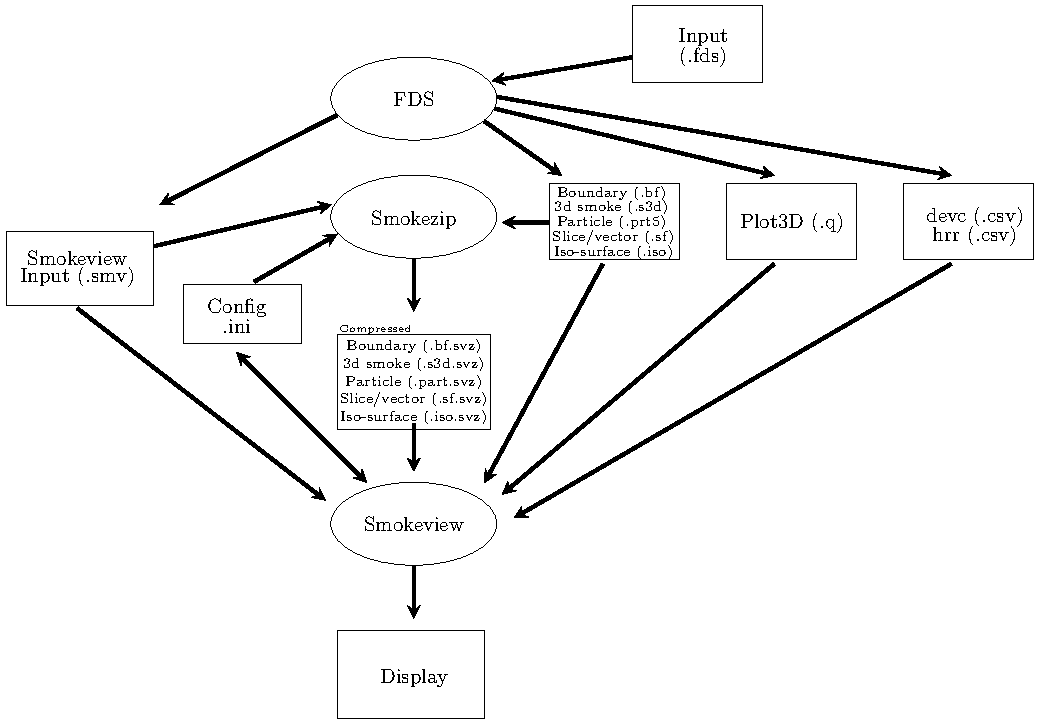
\includegraphics[width=6.5in]{\SMVfigdir/SMV_Overview_Diagram}}
 \caption[FDS file overview]{Diagram illustrating files used and created by the Fire Dynamics
 Simulator (FDS), Smokezip and Smokeview.}
\label{figfdsoverview}%
\end{figure}

\section{Features}

Smokeview is a program designed to visualize numerical
calculations generated by the Fire Dynamics Simulator.
The version of FDS used to run the cases illustrated  in this report
is given by:
\lstinputlisting{SCRIPT_FIGURES/fds.version}
The version of Smokeview described here and used
to generate most figures in this report is given by:
\lstinputlisting{SCRIPT_FIGURES/smokeview.version}

\subsection{Visualizing Data}

Smokeview visualizes data primarily generated by FDS.
Smokeview visualizes data that is both dynamic and static.  Dynamic
data is visualized by animating particle flow (showing
location and {\em values}\ of tracer particles), 2D contour
slices (both within the domain and on solid surfaces) and
3D iso surfaces.  2D contour slices can also be drawn
with colored vectors that use velocity data to show flow
direction, speed and value. Static data is visualized
similarly by drawing 2D contours, vector plots and 3D level
surfaces.

\subsubsection{Particles}\ Lagrangian or moving particles
(Section \ref{section:particles}) may be
used to visualize the flow field. Often these particles represent
smoke or water droplets.  Particles may also be used to represent
people when modeling evacuation flow.

Particle data may also be visualized as streak lines (a particle
drawn where it has been for a short period of time in the past).
Streak lines are a good method for displaying motion using static
images.

\subsubsection{Volumetric - Realistic Smoke}
Smoke and fire (heat release rate per unit volume) are displayed
realistically using a series of partially transparent planes
(Section \ref{section:volsmoke}). The smoke transparencies are
determined by using smoke densities computed by FDS.  The fire and
sprinkler spray transparencies are determined by using a heuristic
based on heat release rate and water density data, again computed
by FDS. Various settings for the 3D smoke option may be set using
the 3D Smoke dialog box found in the {\em Dialogs$>$Data bounds}\ menu.
The windows version of Smokeview uses the graphical processing
unit (GPU) on the video card to perform some of the calculations
required to visualize smoke.

\subsubsection{Slices - 2D contours}
Animated 2D shaded color contour plots (Section
\ref{section:slices}) are used to visualize gas phase information,
such as temperature or density. The contour plots are drawn in
horizontal or vertical planes along any coordinate direction.
Contours can also be drawn in shades of gray.
Shaded contours may also be used to visualize information
computed on solid objects (Section \ref{section:bf}).  These contours are known as boundary files.

Animated 2D shaded color contour plots are also used to
visualize solid phase quantities such as radiative flux or
heat release rate per unit area.

Vector slice files may be visualized if U, V and W velocity slice files are recorded.
Though
similar to solidly shaded contour animations (the vector colors are
the same as the corresponding contour colors), vector animations are better
than solid contour animations for highlighting flow
features since vectors accentuate the direction that flow is occurring.

A 3D region of
data may be visualized using slice files.  Slices may be moved from one plane to
the next just as with Plot3D files (using up/down cursor keys or
page up/page down keys).
3D slices may also be rotated and/or translated by double clicking and
moving the mouse. If the {\tt CTRL}\ or {\tt d}\ key
is also pressed
(press and release the {\tt d}\ key do no hold it down),
the slice moves up and down.
If the {\tt ALT}\ or {\tt f}\ key is pressed,
(press and release the {\tt f}\ key do no hold it down),
the slice moves side to side.
Otherwise, the slice rotates.
Data for 3D slice files are generated by specifying a 3D rather than a
2D region with the {\tt \&SLCF}\ keyword.

Data computed at cell centers rather than interpolated at cell nodes may be visualized.
This is useful for investigating numerical algorithms as the data visualized
has not been interpolated before being seen.

\subsubsection{Surfaces - 3D contours}
Isosurface or 3D level surface animations (Section
\ref{section:isosurface}) may be used to represent flame
boundaries, layer interfaces and various other gas phase
variables. Multiple isocontours may be stored in one file,
allowing one to view several isosurface levels simultaneously.


\subsection{Exploring Data}

\subsubsection{Data Mining}\ The user can analyze and examine the simulated
data by altering its appearance to more easily identify features
and behaviors found in the simulation data. One may flip or
reverse the order of colors in the colorbar and also click in the
colorbar and slide the mouse to highlight data values in the
scene. These options may be found under the {\em Options/Shades}
menu.

The user may click in the timebar and slide the mouse to
change the simulation time displayed. One use for the timebar and colorbar selection modes might be to determine
when smoke of a particular temperature enters a room.

\subsubsection{Data Filtering}\ The File/Bounds Settings...
dialog box allows one to set bounds, to chop or hide data and in the case
of slice file data to time average. (Chapter \ref{chapter:settingoptions})
The data chopping
feature is useful for highlighting data.  A ceiling jet, for example,
may be visualized by hiding ambient temperature
data,  data below a prescribed temperature.
Using time averaging allows one to smooth noisy data over a user selectable time
interval.

\subsubsection{Data coloring}\ Multiple colorbars are available for displaying simulation data.
New colorbars may be created using the colorbar editor (Section \ref{section:colorbar}).
Colorbars may then be adapted to best highlight the simulation data visualized.
Regions in the simulation with certain data values may be highlighted by clicking
on the colorbar.

\subsubsection{Data Compression}\ An option has been added to the
{\em LOAD/UNLOAD}\ menu to compress 3D smoke and boundary
files (Section \ref{ch:smokezip}). The option shells out to the program Smokezip which runs in
the background enabling one to continue to use Smokeview while
files are compressing.

\subsubsection{Data Comparison}\ A stand alone utility program named Smokediff
may be used to compare two FDS cases (Section \ref{ch:smokediff}).
Smokediff generates the difference between corresponding slice and boundary
files for two cases with the same geometry.  Smokediff creates a
{\tt .smv}\ of the differenced data which may then be viewed with Smokeview.


\subsection{Exploring the Scene}

\subsubsection{Motion/View/Render}\ The Motion/View/Render dialog box may be used to
allow more precise control of scene movement and orientation.
Cursor keys have been mapped to scene translation/rotation to
allow easy navigation within the scene.  Viewpoints may be saved for later access.

The first person or eye view mode for moving
allows one to move through a scene more
realistically (Section \ref{section:eyeview}).  Using the cursor keys and the
mouse, one can move through a scene {\em virtually}.

\subsubsection{Stereo views}A method for displaying stereo/3D
images has been implemented that does
not require any specialized equipment such as shuttered glasses or
quad buffered enabled video cards (Section \ref{section:stereo}) .
Stereo pair images are displayed side by side after invoking the option with
the Stereo dialog box or pressing the ``S'' key (upper case).
A 3D view appears by relaxing the eyes, allowing the two images to merge into one.
Pressing the ``S'' key again results in stereo views generated by
displaying red and blue versions of the scene.
Glasses with a red left lens and a blue right lens are required to view the image.

\subsubsection{Scene Clipping}\ It is often difficult to visualize data
in complicated geometries due to the number of obstructed
surfaces. Interior portions of the scene may be seen more easily
by clipping part of the scene away. (Section
\ref{section:clipping})

Clipping discussed above occurs in 3D within the scene.  A
screenshot converted to a PNG or JPEG file may also be clipped or
cropped using the Render portion of the Motion/View/Render
dialog box.

\subsection{Automating the Visualization}
\subsubsection{Virtual Tour}\   A series of checkpoints or key frames
specifying position and view direction may be specified. (Chapter
\ref{chapter:touring}) A smooth path is computed using
Kochanek-Bartels splines~\cite{Moller:02}\ to go through these key
frames so that one may control the position and view direction of
an observer as they move through the simulation. One can then see
the simulation as the observer would. This option is available
under the {\em Tour}\ menu item. Existing tours may be edited and
new tours may be created using the Tour dialog box found in
the {\em Dialogs$>$View}\ menu. Tour settings are stored in the local
configuration file (casename.ini).

\subsubsection{Scripting}\ Smokeview may be run in an unattended mode using
instructions found in a script file. (Chapter
\ref{chapter:scripting}) These instructions direct Smokeview to
load data files, load configuration files, set view points and
time values in order to document a case by rendering the Smokeview
scene into one or more image files. The script file may be created
by Smokeview as a user performs various actions or may be created
by editing a text file.

\subsection{Customizing the Scene}

\subsubsection{Objects}A method for drawing realistic appearing objects such as a heat detector,
smoke detector, sprinkler sensor, etc. has been implemented.
(Chapter \ref{chap:devices}) . Objects are specified in a data
file rather than in Smokeview as C code. This allows one to
customize the look and feel of the objects (to match the types of
detectors/sprinklers that are being used) without requiring code
changes in Smokeview.

\subsubsection{Texture Mapping}\ Image files may be drawn over top
of a blockage, vent or enclosure boundary (Chapter
\ref{chapter:texturemaps}). This is called texture mapping.  This
allows Smokeview scenes to appear more realistic. These image
files may be obtained from the internet, a digital camera, a
scanner or from any other source that generates these file
formats. Image files used for texture mapping should be seamless.
A seamless texture as the name suggests is periodic in both
horizontal and vertical directions. This is an especially
important requirement when textures are tiled or repeated across a
blockage surface.

\subsubsection{Annotating Cases}Text may be added to a scene in order to help document Smokeview
output. (Chapter \ref{section:annotate}) It allows one to place
colored labels at specified locations at specified times. A second
keyword, {\tt TICK}\ keyword places equally spaced tick marks
between specified bounds. These marks along with {\tt LABEL}\ text
may be used to specify length scales in the scene.

The {\em User Tick Settings}\ tab of the Display dialog box
provides an easier way to place ticks with length annotations
along coordinate axes.


%---------------------------------------------------------------------------------
%------------------------ Getting Started -------------------------------------
%---------------------------------------------------------------------------------

\section{Getting Started}

\subsection{Obtaining Smokeview}

Smokeview is available at \hhref{http://fire.nist.gov/fds}.
This site contains links to installation packages for
Windows, Linux and Mac~OS~X operating systems. It also contains documentation for
Smokeview and FDS, sample FDS calculations, software updates and
links for requesting feedback about the software.

After obtaining the setup program, install Smokeview (and FDS)  on the PC by
double-clicking the downloaded
setup program. The setup program then steps through the
program installation. It copies the FDS and Smokeview executables,
sample cases and documentation to the selected directory.  The setup program also
defines PATH variables and associates the {\tt .smv}\ file
extension to the Smokeview program so that one may either type
Smokeview at any command line prompt or double click on any {\tt
.smv}\ file. Smokeview uses the OpenGL graphics library which is a
part of all Windows distributions.

Most computers purchased today are perfectly adequate for running
Smokeview. For Smokeview it is more important to obtain a fast
graphics card than a fast CPU. If the computer will run both FDS
and Smokeview, then a fast CPU is important as well.
For example, the townhouse case used for many examples in this
report consists of about 23000 grid cells.  This case requires
about 10 CPU minutes on a 2.0~GHZ Intel Core i7-2630QM Windows 7
system. Cases with more grid cells and longer simulation times
(the townhouse case simulated 60~s of smoke flow) would clearly
benefit from a faster CPU and more memory which are now relatively
inexpensive.

%---------------------------------------------------------------------------------
%------------------------ Basics  ------------------------------------------------
%---------------------------------------------------------------------------------

\subsection{Running Smokeview}

A typical procedure for using FDS and Smokeview is to:
\begin{enumerate}

\item Create a file named {\tt casename.fds}\ describing the fire
scenario.

\item Type {\tt fds~casename.fds}\ in a command shell to run the
case.

\item Double click on the file named {\tt casename.smv}\ (if on the
PC) or type {\tt smokeview~casename}\ in a command shell (on other
platforms) to start Smokeview.

\item Right clicking within the scene and select a file to load
within the {\em Load/Unload}\ menu.
\end{enumerate}

\noindent This report documents step 3 and 4. Steps 1 and 2 are
documented in the FDS User's Guide~\cite{FDS_Users_Guide}.

Menus in Smokeview are activated by clicking the right mouse
button anywhere within the Smokeview window.  Data files may be
visualized by selecting the desired {\em Load/Unload}\ menu
option. Other menu options are discussed in Appendix
\ref{sectionmenu}. Many menu commands have equivalent keyboard
shortcuts. These shortcuts are listed in Smokeview's {\em Help}\
menu and are described in Appendix \ref{sectionkeyboard}.
Visualization features not controllable through the menus may be
customized by using the Smokeview preference file, \svini,
discussed in Appendix \ref{appendixini}.

Smokeview  is started on a Windows PC by double-clicking the file
named {\tt casename.smv}\ where casename is the name specified by
the {\tt CHID}\ keyword defined in the FDS input data file. Menus
are accessed by clicking with the right mouse button.  The {\em
Load/Unload}\ menu may be used to read in the data files to be
visualized. The {\em Show/Hide}\ menu may be used to change how
the visualizations are presented. For the most part, the menu
choices are self explanatory. Menu items exist for showing and
hiding various simulation elements, creating screen dumps,
obtaining help, etc. Menu items are described in Appendix
\ref{sectionmenu}.

To use Smokeview from a command line, open a command shell. Then
change to the directory containing the FDS case to be viewed and
type:
\begin{lstlisting}
smokeview casename
\end{lstlisting}
where again casename is the name specified by the {\tt CHID}
keyword defined in the FDS input data file. Data files may be
loaded and options may be selected by clicking the right mouse
button and picking the appropriate menu item.


Smokeview opens two windows, one displays the scene and the other
displays status information. Closing either window will end the
Smokeview session.  Multiple copies of Smokeview may be run
simultaneously if the computer has adequate resources.

Normally Smokeview is run during an FDS run, after the run has
completed and as an aid in setting up FDS cases by visualizing
geometric components such as blockages, vents, sensors, etc. One
can then verify that these modeling elements have been defined and
located as intended. One may select the color of these elements
using color parameters in the \svini\ to help distinguish one
element from another. \svini\ file entries are described in
section \ref{appendixini}.

Although specific video card brands cannot be recommended, they
should be high-end due to Smokeview's intensive graphics
requirements. These requirements will only increase in the future
as more features are added.  A video card designed to perform well
for {\em fancy}\ computer games should do well for Smokeview. Some
apparent bugs in Smokeview have been found to be the result of
problems found in video cards on older computers.

\section{Manipulating the Scene}

A Smokeview scene may be rotated or moved by using either the mouse or the Motion/View/Render dialog box.
The scene may be rotated about a point within the scene, usually the scene center, or rotated about the point where the user is located.
In either case, to rotate, click the scene with the left mouse button and drag either horizontally or vertically.
Motion about the
scene center which is the default is called world or global view while motion about the
user location is called eye or first person view. These viewing modes
 may be swapped by pressing the ``e'' key or by selecting
the appropriate radio button in the Motion/View/Render
dialog box.

Similarly, the scene may be translated by clicking the scene with the left mouse button while either the {\tt ALT}\ or {\tt CTRL}\ keys are pressed.
The {\tt ALT} key results in vertical motion of the scene while the {\tt CTRL} key results in motion in and out.

\subsection{World View}

The scene may be rotated or translated using the mouse or
by using controls in the Motion/View/Render dialog box.
This dialog box, illustrated in Fig. \ref{figMOTIONmotion}, is opened
using the {\em Dialogs$>$Motion}\ menu item.

Clicking the left mouse button and dragging horizontally,
vertically or a combination of both results in scene rotation or
translation depending upon whether the CTRL or ALT modifier keys
are pressed or not.\footnote{The Sierra version of the Macintosh OS no longer supports
the {\tt ALT}\ and {\tt CTRL}\ keys when used with the mouse to move the scene.
The {\tt d}\ key may be used
in place of {\tt CTRL}\ key and the {\tt f}\ key may be used in place of the {\tt ALT} key.
Press and release the {\tt d}\ and {\tt f}\ keys do not hold them down.
}

\blist

\hitem{no modifier keys}\ Horizontal mouse movement results in
scene rotation about the Z axis. Vertical mouse movement results
in scene rotation about the X axis.  If the 3-axis rotation option
is selected then mouse movement around the periphery of the scene
results in clockwise or counter clockwise movement about the Y
axis.

\hitem{CTRL key depressed}\ Horizontal mouse movement results in
scene translation from side to side along the X axis. Vertical
mouse movement results in scene translation in and out of the
along the Y axis.

\hitem{ALT key depressed}\ Vertical mouse movement results in scene
translation up and down along the Z axis. Horizontal mouse
movement has no effect.

\elist

\subsection{First Person View}
\label{section:eyeview}
First person view is entered by either pressing the appropriate
radio buttons in the Motion/View/Render dialog box (button
labeled eye centered) or by pressing the ``e'' key until first
person view is obtained. When in {\em eye center}\ mode, several
key mappings have been added, inspired by popular computer games,
to allow for easier movement within the scene. For example, the up
and down cursor keys allow one to move forward or backwards.  The
left and right cursor keys allow one to rotate left or right.
Other keyboard mappings are described in Table \ref{tabKEYS}.

\begin{table}[bph]
\begin{center}
\caption{Keyboard mappings for {\em eye centered}\ or first person scene movement.}
\vspace{0.1in}
\begin{tabular}{|l|l|}
\hline Key &   Description  \\

\hline\hline
up/down cursor & \multirow{2}{*}{move forward/backward}\  \\
w/s &   \\\hline
{\tt ALT}\ + left/right cursor  & \multirow{2}{*}{slide left/right}\ \\
{\tt a/d}\  &  \\ \hline
{\tt ALT}\ + up/down cursor  & move up/down  \\ \hline\hline
left/right cursor  & rotate left/right \\ \hline
{\tt Page Up/Down}\  & look up/down \\ \hline
{\tt Home}\  & look level \\ \hline\hline
\multicolumn{2}{|p{3.5in}|}{Pressing the {\tt SHIFT}\ key while moving, sliding or rotating
results in a  4x speedup of these actions. }\ \\ \hline

\end{tabular}
\label{tabKEYS}
\end{center}
\end{table}

\subsection{Motion Dialog Box}
The Motion dialog box illustrated in Fig \ref{figMOTIONmotion} may also be used to manipulate the
scene. Buttons in the Motion
region of the dialog box allow one to translate or rotate the scene. The
\frameit{Horizontal}\ button is used to translate the scene
horizontally within a horizontal plane (left/right or in/out within the scene).  The
\frameit{Vertical}\ button allows one to translate the scene vertically.
Scene translation and rotations may also be specified by using controls to set x, y, z
coordinates and azimuth, elevation rotation angles within the {\em Specify Orientation}\ panel.
Within this same panel one may also specify whether the gravity vector (usually pointed down) is visualized and/or used to draw the scene.

The \frameit{Rotate about}\ selection list allows one to change the center of rotation.
Rotation center choices are: the scene center, denoted as {\em world center}\ in this list, the center of each mesh and a center specified by the user.
Changing the rotation center is useful for cases where the portion of the scene being viewed is far away from the currently used rotation center.
To allow for easier changes, the rotation center may be made visible (drawn as a small black sphere) by selecting the {\em Show}\ checkbox within the {\em rotation center panel}.  The rotation center may be changed by using the
{\em x, y, z}\ spinners below this checkbox.

\begin{figure}[bph]
\centerline{
\begin{tabular}{cc}
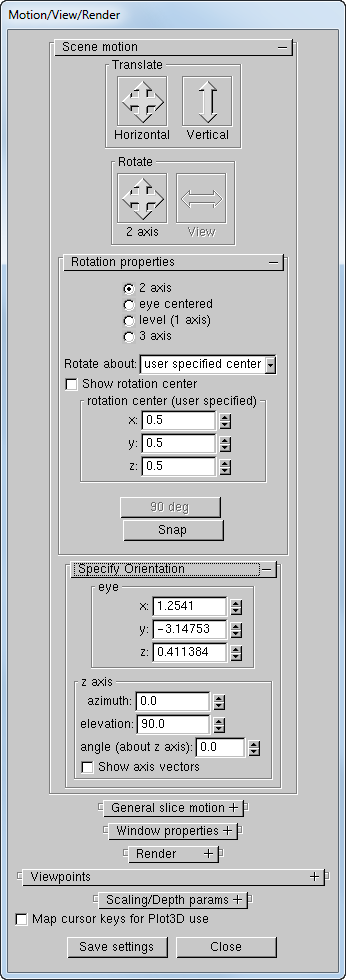
\includegraphics[width=2.104166667in]{\SMVfigdir/figMOTION}
\end{tabular}
}\ \caption[Dialog box for controlling scene motion.]{Dialog box for controlling scene motion. To rotate the scene, select the rotation type
then select and move the mouse in the  rotation control.  One may also select where to rotate about (scene center, any mesh center or user specified center). To translate the scene, select and move the mouse in the horizontal or vertical control.}\ \label{figMOTIONmotion}
\end{figure}

%---------------------------------------------------------------------------------
%---------------Realistic or Qualitative Visualization - 3D Smoke--------------
%---------------------------------------------------------------------------------

\chapter{Visualizing Smoke}

\section{Tracers and Streaklines}

\renewcommand{\figheight}{1.4in}

\label{section:particles}\ Particle files contain the locations of
tracer particles used to visualize the flow field. Figure
\ref{figparticle}\ shows several snapshots of a developing kitchen
fire visualized by using particles where particles are colored
black. If present, sprinkler water droplets would be colored blue.
Particles are stored in files ending with the extension {\tt
.prt5}\ and are displayed by selecting the particle file entry from
the {\em Load/Unload}\ menu.

Streaklines are a technique for showing motion in a still image.
Figure \ref{figstreak}\ shows a snapshot of the same kitchen fire
using streak lines instead of particles.  The streaks begin at 9~s
and end at 10~s.


\begin{figure}[bph]
\begin{center}
\begin{tabular}{cc}
 \includegraphics[height=\figheightA]{SCRIPT_FIGURES/thouse5_part_005}&
 \includegraphics[height=\figheightA]{SCRIPT_FIGURES/thouse5_part_010}\\
 5.0 s&10.0 s\\
\includegraphics[height=\figheightA]{SCRIPT_FIGURES/thouse5_part_030}&
\includegraphics[height=\figheightA]{SCRIPT_FIGURES/thouse5_part_060}\\
30.0 s&60.0 s\\
\end{tabular}
\end{center}

\caption{Townhouse kitchen fire visualized using tracer
particles.}
\label{figparticle}%
\end{figure}

\begin{figure}[bph]
\begin{center}
\includegraphics[height=4.0in]{SCRIPT_FIGURES/thouse5_streak_010}
\end{center}

\caption{Townhouse kitchen fire visualized using streak lines. The
{\em pin heads}\ shows flow conditions at 10~s, the corresponding
{\em tails}\ shows conditions 1.0~s earlier.}
\label{figstreak}%
\end{figure}

Particle file data may be converted to an isosurface using
Smokezip.  The isosurface location is defined in terms of particle
density and the isosurface color is defined in terms of averaged
particle values. See  Chapter \ref{ch:smokezip}\ for more details
on using Smokezip for generating isosurface files from particle
files and Section \ref{section:isosurface}\ for some examples.

\section{Realistic}
\label{section:volsmoke}\ FDS generates several data files
visualized by Smokeview. Each file type may be loaded or unloaded
using the {\em Load/Unload}\ menu described in Appendix
\ref{sectload}. Visualizations produced by these data files are
described in this and the following sections. The format used to
store each of the data files is given in the FDS User's
Guide~\cite{FDS_Users_Guide}.

Visualizing smoke realistically is a daunting challenge for at
least three reasons. First, the storage requirements for
describing smoke can easily exceed the disk capacities of present
32 bit operating systems such as Linux, i.e., file sizes can easily
exceed 2 gigabytes. Second, the computation required both by the
CPU and the video card to display each frame can easily exceed
0.1~s, the time corresponding to a 10~frame/s display rate. Third,
the physics required to describe smoke and its interactions with
itself and surrounding light sources is complex and
computationally intensive. Therefore, approximations and
simplifications are required to display smoke rapidly.

Smoke visualization techniques such as tracer particles or shaded
2D contours are useful for quantitative analysis but not suitable
for virtual reality applications, where displays need to be
realistic and fast as well as accurate. The approach taken by
Smokeview is to display a series of parallel planes.  Each plane
is colored black (for smoke) with transparency values pre-computed
by FDS using time dependent soot densities also computed by FDS
corresponding to the grid spacings of the simulation. The
transparencies are adjusted in real time by Smokeview to account
for differing path lengths through the smoke as the view direction
changes. The graphics hardware then combines the planes together
to form one image.

Fire by default is colored a dark shade of orange wherever the
computed heat release rate per unit volume exceeds a user-defined
cutoff value.  The visual characteristics of fire are not
automatically accounted for.  The user though may use the 3D
Smoke dialog box to change both the color and transparency of
the fire for fires that have non-standard colors and opacities.

The windows version of Smokeview has the option of using the GPU
or graphics programming unit to perform some of the calculations
required to visualize realistic smoke.  These calculations consist
of adjusting the smoke opaqueness as pre-computed in FDS to
account for off-axis viewing directions. The GPU performs the
computations in parallel while the former method using the CPU
performs them sequentially.  For many (but not all) cases, the use
of the GPU results in a smoke drawing speed up of 50 \% or more.
This option is turned on or off by pressing the {\tt G}\ key.


Figure \ref{figsmoke3d}\ illustrates a visualization of realistic
smoke.

\begin{figure}[bph]
\begin{center}
\begin{tabular}{cc}
 \includegraphics[height=\figheightA]{SCRIPT_FIGURES/thouse5_smoke_005}&
 \includegraphics[height=\figheightA]{SCRIPT_FIGURES/thouse5_smoke_010}\\
 5.0 s&10.0 s\\
\includegraphics[height=\figheightA]{SCRIPT_FIGURES/thouse5_smoke_030}&
\includegraphics[height=\figheightA]{SCRIPT_FIGURES/thouse5_smoke_060}\\
30.0 s&60.0 s\\
\end{tabular}
\end{center}
\caption{Smoke3d file snapshots at various times in a simulation
of a townhouse kitchen fire.
  }
\label{figsmoke3d}%
\end{figure}

\chapter{Visualizing Data Quantitatively}

\section{Coloring data}Smokeview uses a 1D texture map for coloring data occurring in
slice, boundary and Plot3D files. 1D texture maps or colorbars may
be selected using the Data coloring dialog box illustrated in Fig. \ref{figDatacoloring}.
This dialog box is used to control how data is colored.
One may select the mapping used to associate data with color (a colorbar).
One may also select the colors used to color extreme data, data with values greater
the maximum or smaller than the minimum (smallest and greatest colorbar data labels).
When the colorbar is selected with the mouse a portion of it changes color to black.
Data in the scene with the same values are also colored black.
The width of the selection region (default 5 pixels) may be selected with this dialog box.
Other data coloring properties such as transparency, order of the colorbar may also be selected.

\begin{figure}[bph]
\centerline{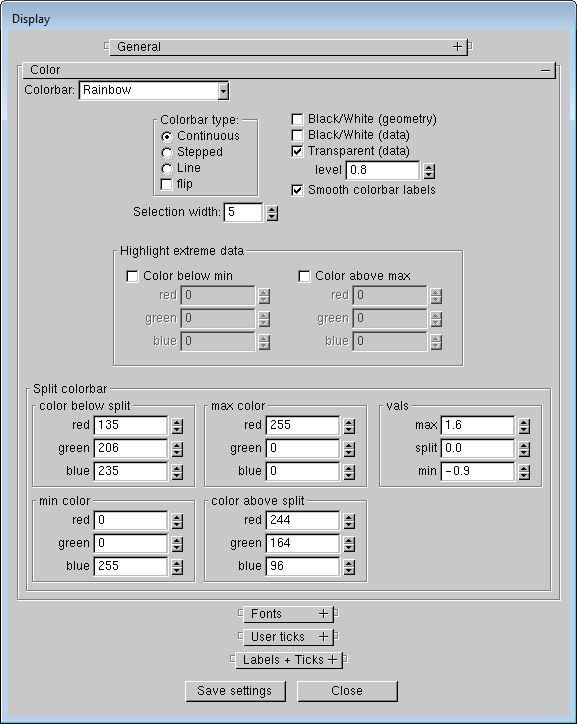
\includegraphics[width=4.00694444in]{\SMVfigdir/figDatacoloring}
}\ \caption [Dialog Box for selecting colorbars.] {Dialog
box for selecting colorbars.  The selected colorbar may be modified by
shading it continuously, stepped or as a series of discrete lines.  The
colorbar may also be converted to shades of gray.  Colors for
extreme data (data outside of specified bounds) may be specified.
A split colorbar may be specified using one range of colors between the minimum
value and the split and another range of colors between the split and the maximum value.}
\label{figDatacoloring}
\end{figure}

\begin{figure}[bph]
\begin{center}
\begin{tabular}{ccc}
\includegraphics[height=\figheightAbar]{SCRIPT_FIGURES/thouse5_slicesplit_005}&
\includegraphics[height=\figheightAbar]{SCRIPT_FIGURES/thouse5_slicesplit_010}\\
5.0 s&10.0 s\\
\includegraphics[height=\figheightAbar]{SCRIPT_FIGURES/thouse5_slicesplit_030}&
\includegraphics[height=\figheightAbar]{SCRIPT_FIGURES/thouse5_slicesplit_060}&\\
30.0 s&60.0 s
&\raisebox{0.0ex}[0pt]{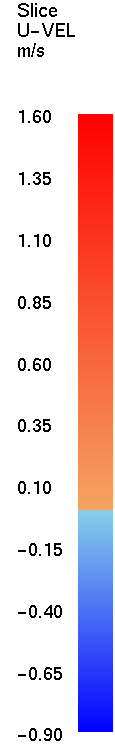
\includegraphics[height=5.0in]{\SMVfigdir/colorbar_uvel}}\\
\end{tabular}
\caption [Slice file snapshots of shaded U velocity contours using a colorbar with a split at 0.0~m/s.]
{Slice file snapshots of shaded U velocity contours at various
times in a simulation using a colorbar with a split at 0.0~m/s. Velocities greater than 0.0~m/s are colored with shades of red.
Velocities less than 0.0~m/s are colored with shades of blue. }
\label{figslicesplit}%
\end{center}
\end{figure}


A colorbar defined with a split may also be specified with this dialog box.  One range of colors are specified between the minimum
data value and the split value and another range of colors are specified between the split value and the maximum value. This is useful when highlighting
data that has a special property, for example a tenability temperature criteria or where flow velocity reverses.
Figure \ref{figslicesplit} illustrates a scene using a colorbar with a split at 0.0~m/s. Velocities greater than 0.0~m/s are colored with shades of red.
Velocities less than 0.0~m/s are colored with shades of blue.

Fig. \ref{fignewslice}\ illustrates how interpolating color within the colorbar
improves the visualization.
Colors are crisper and sharper, more
accurately representing the underlying data. This is most
noticeable when selecting the colorbar with the mouse.
This causes a portion of the colorbar to turn black and the
corresponding region in the scene to also turn black.  The
black color is accurate to the pixel so this feature may be used
to highlight regions of interest. The improved accuracy is a
result of the way color interpolations are performed.  Colors
are interpolated within the colorbar using a 1D texture map.  Color interpolations with
the former method occurred within the color cube.

Note, due to the way that transparent objects are drawn (from back to front),
3D Smoke/Fire and transparent slices may not display
properly when shown at the same time.

\begin{figure}[bph]
\begin{center}
\begin{tabular}{ccc}
\includegraphics[height=3.5in]{../SMV_Verification_Guide/SCRIPT_FIGURES/plume5c_notexturebar}&
\includegraphics[height=3.5in]{../SMV_Verification_Guide/SCRIPT_FIGURES/plume5c_texturebar}\\
colors interpolated using a 3D color cube&colors interpolated using a 1D texture colorbar\\
\end{tabular}
\caption [Slice file snapshots illustrating two methods for mapping data to color.] {Slice file snapshots illustrating two methods for mapping data to color.}
\label{fignewslice}%
\end{center}
\end{figure}

\section{2D Shaded Contours and Vector Slices - Slice Files}
\label{section:slices}
\subsection{Axis aligned slices}

Slice files contain results recorded within a rectangular array of
grid points at each recorded time step. Continuously shaded
contours are drawn for simulation quantities such as temperature,
gas velocity and heat release rate. Figure \ref{figslice}\ shows
several snapshots of a vertical animated slice where the slice is
colored according to gas temperature. Slice files have file names
with extension {\tt .sf}\ and are displayed by selecting the
desired entry from the {\em Load/Unload}\ menu.

All slice files oriented along the same plane (x, y and/or z directions) may be loaded
with one mouse click by choosing the desired orientation from the {\em Slice}
portion of the {\em Load/Unload}\ menu.  These menu entries do not exist in the Multi-Slice menu.
However, when selected from the {\em Slice}\ menu, Smokeview will load all x/y/z oriented multi-slices.


\begin{figure}[bph]
\begin{center}
\begin{tabular}{ccc}
\includegraphics[height=\figheightAbar]{SCRIPT_FIGURES/thouse5_slice_005}&
\includegraphics[height=\figheightAbar]{SCRIPT_FIGURES/thouse5_slice_010}\\
5.0 s&10.0 s\\
\includegraphics[height=\figheightAbar]{SCRIPT_FIGURES/thouse5_slice_030}&
\includegraphics[height=\figheightAbar]{SCRIPT_FIGURES/thouse5_slice_060}&\\
30.0 s&60.0 s
&\raisebox{0.0ex}[0pt]{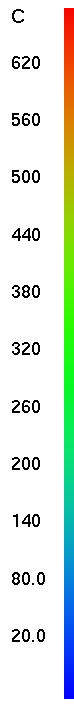
\includegraphics[height=5.0in]{\SMVfigdir/colorbar_20_620}}\\
\end{tabular}
\caption [Slice file snapshots of shaded temperature contours.]
{Slice file snapshots of shaded temperature contours at various
times in a simulation. These contours were generated by adding
``{\tt \&SLCF PBY=1.5, QUANTITY='TEMPERATURE' /}'' to the FDS
input file. }
\label{figslice}%
\end{center}
\end{figure}

\indent To specify in FDS a vertical slice 1.5~m from the $y=0$
boundary colored by temperature, use the line:
\begin{lstlisting}[basicstyle=\ttfamily]
&SLCF PBY=1.5 QUANTITY='TEMPERATURE' /
\end{lstlisting}
A more complete list of output quantities may be found in
Ref.~\cite{FDS_Users_Guide}.

\paragraph{Vector slices}Animated vectors are displayed using data contained in two or more
slice files.  The direction and length of the vectors are
determined from the $U$, $V$ and/or $W$ velocity slice files. The
vector colors are determined from the file (such as temperature)
selected from the {\em Load/Unload}\ menu. The length of the
vectors can be adjusted by pressing the {\tt `a'}\ key. For cases
with a fine grid, the number of vectors may be overwhelming.
Vectors may be skipped by pressing the {\tt `s'}\ key.  Figure
\ref{figvslice}\ shows a sequence of vector slices corresponding to
the shaded temperature contours found in Fig.~\ref{figslice}.

\begin{figure}[bph]
\begin{center}
\begin{tabular}{ccc}
\includegraphics[height=\figheightAbar]{SCRIPT_FIGURES/thouse5_vslice_005}&
\includegraphics[height=\figheightAbar]{SCRIPT_FIGURES/thouse5_vslice_010}\\
5.0 s&10.0 s\\
\includegraphics[height=\figheightAbar]{SCRIPT_FIGURES/thouse5_vslice_030}&
\includegraphics[height=\figheightAbar]{SCRIPT_FIGURES/thouse5_vslice_060}\\
30.0 s&60.0 s
&\raisebox{0.0ex}[0pt]{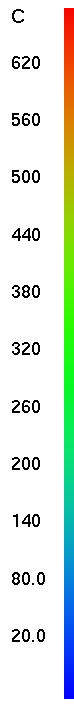
\includegraphics[height=5.0in]{\SMVfigdir/colorbar_20_620}}\\
\end{tabular}
\end{center}
\caption [Vector slice file snapshots of shaded vector plots.]
{Vector slice file snapshots of shaded vector plots. These vector
plots were generated by using ``{\tt \&SLCF
PBY=1.5,QUANTITY='TEMPERATURE',VECTOR=.TRUE. /}''.}
\label{figvslice}%
\end{figure}

Similar to slice files, all vector slice files oriented along the same plane (x, y and/or z directions) may be loaded
with one mouse click by choosing the desired orientation from the {\em Vector Slice}
portion of the {\em Load/Unload}\ menu.  These menu entries do not exist in the Vector Multi-Slice menu.
However, when selected from the {\em Vector Slice}\ menu, Smokeview will load all x/y/z oriented multi-slices.

To generate the extra velocity files needed to view vector
animations, add {\tt VECTOR=.TRUE.}\ to the above {\tt \&SLCF}\ line
to obtain:
\begin{lstlisting}
&SLCF PBY=1.50,QUANTITY='TEMPERATURE',VECTOR=.TRUE. /
\end{lstlisting}

\subsection{3D slices}
The user may visualize a 3D region of data using slice files.
To specify a cube of data from 1.0 to 2.0 in each
of the X, Y and Z directions in FDS, use the line:
\begin{lstlisting}
&SLCF XB=1.0,2.0,1.0,2.0,1.0,2.0 QUANTITY='TEMPERATURE' /
\end{lstlisting}

A slice from the resulting slice file
may be moved from one plane to the next just as with Plot3D
files (using left/right, up/down cursor keys or page up/page down
keys).  3D slices and 3D vector slices may also be oriented arbitrarily.
To make these slices visible press the {\tt w}\ key.  Examples of
these slices are illustrated in Figs. \ref{figgslice}\ and \ref{figvgslice}.
These slice may also be oriented in arbitrary positions and directions by
double clicking within the scene.  While holding down the mouse after double clicking,
move the mouse from
side to side or up and down to rotate the general slice.  Double clicking and moving
the mouse vertically while holding down the {\tt ALT}\
key causes the center of rotation for the general slice to move up and down.
Double clicking and moving the mouse horizontally and vertically while holding down
the {\tt SHIFT}\ key causes the center of rotation for the general slice to move along
the {\tt X}\ and {\tt Y}\ axis respectively.

The position and orientation of 3D slices may be manipulated using the Slice motion
portion of the Motion/View/Render dialog box as illustrated
in Fig. \ref{figGSLICE}.

\begin{figure}[bph]
\begin{center}
\begin{tabular}{ccc}
\includegraphics[height=\figheightAbar]{SCRIPT_FIGURES/thouse5_gslice1}&
\includegraphics[height=\figheightAbar]{SCRIPT_FIGURES/thouse5_gslice2}\\
\includegraphics[height=\figheightAbar]{SCRIPT_FIGURES/thouse5_gslice3}&
\includegraphics[height=\figheightAbar]{SCRIPT_FIGURES/thouse5_gslice4}&\\
&&\raisebox{0.0ex}[0pt]{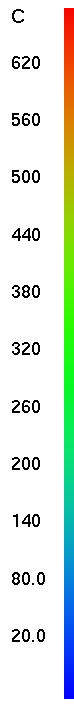
\includegraphics[height=5.0in]{\SMVfigdir/colorbar_20_620}}\\
\end{tabular}
\caption [General oriented temperature slices.]
{
Slices from a 3D temperature slice file at 60~s displayed using four orientations.
3D slices may be re-oriented by double clicking and dragging the mouse
or by changing settings in the Motion/View/Render dialog box.
These images were generated using
``{\tt \&SLCF XB=0.0,6.4,0.0,8.0,0.0,4.8, QUANTITY='TEMPERATURE' /}'' in an FDS
input file. }
\label{figgslice}%
\end{center}
\end{figure}

\begin{figure}[bph]
\begin{center}
\begin{tabular}{ccc}
\includegraphics[height=\figheightAbar]{SCRIPT_FIGURES/thouse5_vgslice1}&
\includegraphics[height=\figheightAbar]{SCRIPT_FIGURES/thouse5_vgslice2}\\
\includegraphics[height=\figheightAbar]{SCRIPT_FIGURES/thouse5_vgslice3}&
\includegraphics[height=\figheightAbar]{SCRIPT_FIGURES/thouse5_vgslice4}&\\
&&\raisebox{0.0ex}[0pt]{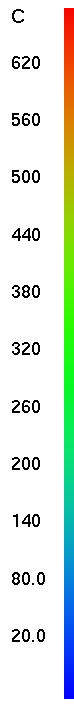
\includegraphics[height=5.0in]{\SMVfigdir/colorbar_20_620}}\\
\end{tabular}
\caption [General oriented vector temperature slices.]
{
Vector 3D temperature slices at 60~s displayed using four orientations.
3D vector slices may be re-oriented by double clicking and dragging the mouse
or by changing settings in the Motion/View/Render dialog box.
These images were generated using
``{\tt \&SLCF XB=0.0,6.4,0.0,8.0,0.0,4.8, QUANTITY='TEMPERATURE', VECTOR=.TRUE./}'' in an FDS
input file. }
\label{figvgslice}%
\end{center}
\end{figure}

\begin{figure}[bph]
\centerline{
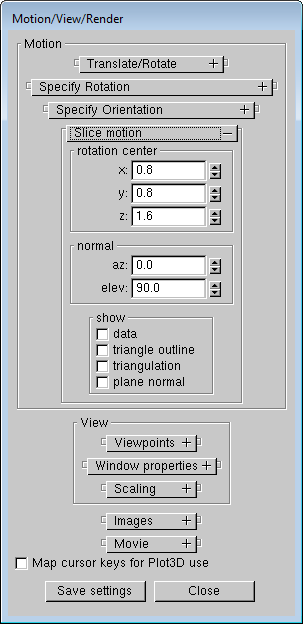
\includegraphics[width=2.10416666in]{\SMVfigdir/figGSLICE}
}
\caption[Dialog box for controlling the orientation of a 3D slice file.]{Dialog box for controlling the orientation of a 3D slice file.}
\label{figGSLICE}
\end{figure}

\subsection{Wind Roses}
A wind rose displays a 2D summary of how flow velocities are distributed at a point over some period of time. Data for a wind rose is generated by specifying devices for U, V and W components of velocity using {\tt \&DEVC}\ keywords such as

\begin{verbatim}
&DEVC XYZ=1.2,0.8,1.0 QUANTITY='U-VELOCITY' /
&DEVC XYZ=1.2,0.8,1.0 QUANTITY='V-VELOCITY' /
&DEVC XYZ=1.2,0.8,1.0 QUANTITY='W-VELOCITY' /
\end{verbatim}

\noindent in an FDS input file.  Smokeview creates a two dimensional histogram recording the distribution of wind speeds and direction.
The user can then set various viewing options using the wind rose dialog box illustrated in Figure \ref{figWINDROSE}. Figure \ref{figWINDROSEplots}
illustrates wind roses at several locations drawn in horizontal (xy) and vertical (xz) planes.

\begin{figure}[bph]
\centerline{
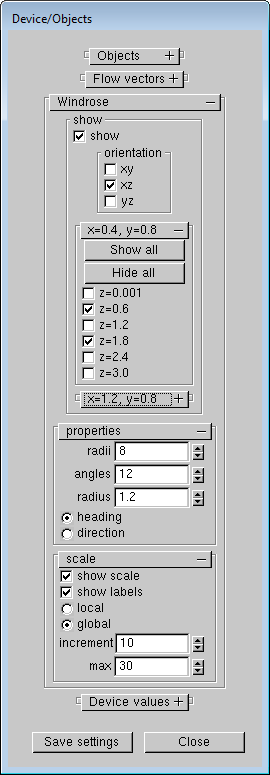
\includegraphics[width=1.875in]{\SMVfigdir/figWINDROSE}
}
\caption[Dialog Box for setting wind rose options]
{Dialog Box for setting wind rose options}
\label{figWINDROSE}
\end{figure}

\begin{figure}[bph]
\begin{center}
\begin{tabular}{cc}
\includegraphics[width=3.0in]{SCRIPT_FIGURES/windrose_xz}&
\includegraphics[width=3.0in]{SCRIPT_FIGURES/windrose_xy}\\
XZ&XY
\end{tabular}
\end{center}
\caption[Wind roses visualizing velocity flow distributions in XZ and XY planes at several locations]
{Wind roses visualizing velocity flow distributions in XZ and XY planes at several locations}
\label{figWINDROSEplots}
\end{figure}

\subsection{Fractional effective dose (FED) slices}
The fractional effective dose (FED), developed by Purser~\cite{SFPE:Purser},
is an estimate of human incapacitation
due to a limited set of combustion gases.
FED index data is computed by Smokeview using CO, $\mathrm{CO_2}$ and $\mathrm{O_2}$ gas
concentration data computed by FDS.
This data is made available to Smokeview in the form of slice files.
Smokeview computes FED data using
\be
\mathrm{FED}_\mathrm{tot}\ = \mathrm{FED}_\mathrm{CO}
\times \mathrm{HV}_\mathrm{CO_2}\ + \mathrm{FED}_\mathrm{O_2}
\ee
where $\mathrm{FED}_\mathrm{tot}$ is the total FED,
$\mathrm{FED}_\mathrm{CO}$ is the FED due to CO,
$\mathrm{HV}_\mathrm{CO_2}$ is a hyper-ventilating factor
applied to CO and $\mathrm{FED}_\mathrm{O_2}$
is the FED due to $\mathrm{O_2}$.
The species data slices used to compute an FED slice needs to be specified at the
same location.  To generate an FED slice at $y=1.6$, specify the following species slices in the input file
\begin{lstlisting}
&SLCF PBY=1.6,QUANTITY='VOLUME FRACTION' SPEC_ID='CARBON DIOXIDE' /
&SLCF PBY=1.6,QUANTITY='VOLUME FRACTION' SPEC_ID='CARBON MONOXIDE' /
&SLCF PBY=1.6,QUANTITY='VOLUME FRACTION' SPEC_ID='OXYGEN' /
\end{lstlisting}

FED computations are stored by Smokeview in slice files for subsequent use.
Since this computation
is performed in Smokeview using data only found in the slices files, time step intervals
should be chosen to ensure accuracy.  Figure \ref{figfedslice}\ illustrates
an FED slice file at several times.  The FED colorbar is split at values of 0.3, 1.0 and 3.0.  When FED slices are displayed using the FED colorbar (colorbar illustrated in Figure \ref{figfedslice}), Smokeview computes color levels assuming a minimum FED level of 0.0 and a maximum level of 3.0.  To display FED data using other data bounds, a different colorbar needs to be chosen.

\begin{figure}[bph]
\begin{center}
\begin{tabular}{ccc}
\includegraphics[height=\figheightAbar]{SCRIPT_FIGURES/thouse5_fed_z1p5_slice_005}&
\includegraphics[height=\figheightAbar]{SCRIPT_FIGURES/thouse5_fed_z1p5_slice_010}\\
5.0 s&10.0 s\\
\includegraphics[height=\figheightAbar]{SCRIPT_FIGURES/thouse5_fed_z1p5_slice_030}&
\includegraphics[height=\figheightAbar]{SCRIPT_FIGURES/thouse5_fed_z1p5_slice_060}&\\
30.0 s&60.0 s
&\raisebox{0.0ex}[0pt]{\includegraphics[height=5.0in]{\SMVfigdir/colorbar_fed}}\\
\end{tabular}
\caption [FED slices.]
{FED slices.
These contours were generated using CO, $\mathrm{CO_2}$ and $\mathrm{O_2}$ data slices.
}
\label{figfedslice}%
\end{center}
\end{figure}

\subsection{Duplicate Slices}
FDS outputs duplicate slices whenever a {\tt \&SLCF}\ entry is specified where two meshes coincide.  One set of slices is output for each mesh.  Using the Slice/Duplicates panel of the File/Bounds dialog box, illustrated in Figure \ref{fig:sliceduplicate}, one may specify whether to keep all duplicate slices, keep the finely gridded slices or keep the coarsely gridded slices.  One may similarly specify preferences for vector slice files. By default smokeview keeps only finely gridded slices and keeps all vector slices (so one may diagnose possible flow problems).

FDS also outputs duplicate slices when two or more identical {\tt \&SLCF}\ entries are specified in the input ({\tt .fds}) file.  Smokeview ignores these duplicate slices when processing the {\tt .smv} file.

\begin{figure}[bph]
\centerline{
\includegraphics[width=2.390305555in]{\SMVfigdir/figsliceduplicate}
}
\caption[Dialog box for specifying duplicate slice visibility.]{Dialog box for specifying duplicate slice visibility.}
\label{fig:sliceduplicate}
\end{figure}


\section{2D Shaded Contours on Solid Surfaces - Boundary Files}
\label{section:bf}
Boundary files contain simulation data recorded at blockage or
wall surfaces. Continuously shaded contours are drawn for
quantities such as wall surface temperature, radiative flux, etc.
Figure \ref{figboundary}\ shows several snapshots of a boundary
file animation where the surfaces are colored according to their
temperature. Boundary files have file names with extension {\tt
.bf}\ and are displayed by selecting the desired entry from the
{\em Load/Unload}\  menu. Figure \ref{figtruncboundary}\ shows the
same snapshots as in Fig. \ref{figboundary}\ except that data
below 200~\degC\ is chopped.
\begin{figure}[bph]
\begin{center}
\begin{tabular}{ccc}
\includegraphics[height=\figheightAbar]{SCRIPT_FIGURES/thouse5_bound_005}&
\includegraphics[height=\figheightAbar]{SCRIPT_FIGURES/thouse5_bound_010}\\
5.0 s&10.0 s\\
\includegraphics[height=\figheightAbar]{SCRIPT_FIGURES/thouse5_bound_030}&
\includegraphics[height=\figheightAbar]{SCRIPT_FIGURES/thouse5_bound_060}\\
30.0 s&60.0 s
&\raisebox{0.0ex}[0pt]{\includegraphics[height=5.0in]{\SMVfigdir/colorbar_20_620}}\\
\end{tabular}
\end{center}
\caption [Boundary file snapshots of shaded wall temperatures
contours (cell averaged data).] {Boundary file snapshots of shaded
wall temperatures (cell averaged data). These snapshots were
generated by using ``{\tt\&BNDF QUANTITY='WALL\_TEMPERATURE'/}''.
}
\label{figboundary}%
\end{figure}

\begin{figure}[bph]
\begin{center}
\begin{tabular}{ccc}
\includegraphics[height=\figheightAbar]{SCRIPT_FIGURES/thouse5_bound_trunc_005}&
\includegraphics[height=\figheightAbar]{SCRIPT_FIGURES/thouse5_bound_trunc_010}\\
5.0 s&10.0 s\\
\includegraphics[height=\figheightAbar]{SCRIPT_FIGURES/thouse5_bound_trunc_030}&
\includegraphics[height=\figheightAbar]{SCRIPT_FIGURES/thouse5_bound_trunc_060}\\
30.0 s&60.0 s
&\raisebox{0.0ex}[0pt]{\includegraphics[height=5.0in]{\SMVfigdir/colorbar_20_620}}\\
\end{tabular}
\end{center}
\caption [Boundary file snapshots of truncated shaded wall
temperatures contours (cell averaged data).] {Boundary file
snapshots of truncated shaded wall temperatures (cell averaged
data).  Data values are truncated or chopped below 200~\degC.
These snapshots were generated by using ``{\tt\&BNDF
QUANTITY='WALL\_TEMPERATURE'/}''. }
\label{figtruncboundary}%
\end{figure}

\begin{figure}[bph]
\begin{center}
\begin{tabular}{ccc}
\includegraphics[height=\figheightAbar]{SCRIPT_FIGURES/thouse5_bound_cell_005}&
\includegraphics[height=\figheightAbar]{SCRIPT_FIGURES/thouse5_bound_cell_010}\\
5.0 s&10.0 s\\
\includegraphics[height=\figheightAbar]{SCRIPT_FIGURES/thouse5_bound_cell_030}&
\includegraphics[height=\figheightAbar]{SCRIPT_FIGURES/thouse5_bound_cell_060}\\
30.0 s&60.0 s
&\raisebox{0.0ex}[0pt]{\includegraphics[height=5.0in]{\SMVfigdir/colorbar_20_620}}\\
\end{tabular}
\end{center}
\caption [Boundary file snapshots of shaded wall temperatures
contours (cell centered data).] {Boundary file snapshots of shaded
wall temperatures (cell centered data) These snapshots were
generated by using ``{\tt\&BNDF QUANTITY='WALL\_TEMPERATURE'
CELL\_CENTERED=.TRUE. /}''. }
\label{figboundary_cell_centered}%
\end{figure}
A boundary file containing wall temperature data may be generated
by using:
\begin{lstlisting}
&BNDF QUANTITY='WALL TEMPERATURE' /
\end{lstlisting}
Loading a boundary file is a memory intensive operation.  The
entire boundary file is read in to determine the minimum and
maximum data values.  These bounds are then used to convert four
byte floats to one byte color indices.  To drastically reduce the
memory requirements, simply specify the minimum and maximum data
bounds using the Set Bounds dialog box.  This should be
done before loading the boundary file data.  When this is done,
memory for the boundary file data is allocated for only one time
step rather than for all time steps.

\section{3D Contours - Isosurface Files}
\label{section:isosurface}
\begin{figure}[bph]
\begin{center}
\begin{tabular}{cc}
\includegraphics[height=\figheightA]{SCRIPT_FIGURES/thouse5_iso_005}&
\includegraphics[height=\figheightA]{SCRIPT_FIGURES/thouse5_iso_010}\\
5.0 s&10.0 s\\
\includegraphics[height=\figheightA]{SCRIPT_FIGURES/thouse5_iso_030}&
\includegraphics[height=\figheightA]{SCRIPT_FIGURES/thouse5_iso_060}\\
30.0 s&60.0 s
\end{tabular}
\end{center}
\caption [Isosurface file snapshots of temperature levels. ]

{ Isosurface file snapshots of temperature levels. The orange
surface is drawn where the air/smoke temperature is 30~\degC\ and
the white surface is drawn where the air/smoke temperature is
100~\degC. These snapshots were generated by adding ``{\tt\&ISOF
QUANTITY='TEMPERATURE',VALUE(1)=30.0,VALUE(2)=100.0 /}'' to the
FDS input file.}
\label{figiso}%
\end{figure}

The surface where a quantity such as temperature attains a given
value is called an isosurface. An isosurface is also called a
level surface or 3D contour. Isosurface files contain data
specifying isosurface locations for a given quantity at one or
more levels. These surfaces are represented as triangles.
Isosurface files have file names with extension .iso and are
displayed by selecting the desired entry from the {\em
Load/Unload}\ menu.

Isosurfaces are specified in the FDS input file with the {\tt
\&ISOF}\ keyword.  To specify isosurfaces for temperatures of
30\degC\ and 100\degC\ as illustrated in Fig. \ref{figiso}\ add
the line:
\begin{lstlisting}
&ISOF QUANTITY='TEMPERATURE', VALUE(1)=30.0, VALUE(2)=100.0 /
\end{lstlisting}
to the FDS input file.  A complete list of isosurface quantities
may be found in Ref.~\cite{FDS_Users_Guide}

\subsection{Isosurfaces from particle files}
The Smokezip -part2iso option may be used to generate isosurfaces from particle data.
Isosurface locations indicate a boundary separating particle and
no-particle regions, i.e., wherever particle density is 0.5
particles per grid cell.  Isosurface  coloring is determined using
averaged particle data.  Representing particle data with an
isosurface is useful when particles are used to model objects such
as trees especially when the objects are viewed up close.  See
Chapter \ref{ch:smokezip}\ for more details on generating
isosurface files from particle files.  Figure \ref{figisoparticle}
shows a snapshot of a fire plume generated using particles and the command
\begin{lstlisting}
smokezip -part2iso plumeiso
\end{lstlisting}
The plume is visualized using both particles and an isosurface
generated from these same particles.


\begin{figure}[bph]
\begin{center}
\begin{tabular}{cc}
\includegraphics[height=3.75in]{../SMV_Verification_Guide/SCRIPT_FIGURES/plumeiso_prt5_10}&
\includegraphics[height=3.75in]{../SMV_Verification_Guide/SCRIPT_FIGURES/plumeiso_prt5_iso_10}\\
particles at 10.0~s&particle isosurface at 10.0~s\\
\includegraphics[height=3.75in]{../SMV_Verification_Guide/SCRIPT_FIGURES/plumeiso_prt5_30}&
\includegraphics[height=3.75in]{../SMV_Verification_Guide/SCRIPT_FIGURES/plumeiso_prt5_iso_30}\\
particles at 30.0~s&particle isosurface at 30.0~s\\
\end{tabular}
\end{center}
\caption{Fire plume visualized using particles and isosurfaces
generated from  particles.}
\label{figisoparticle}%
\end{figure}

\subsection{Isosurfaces from fractional effective dose data (generated by Smokeview)}
As with 2D slices, Smokeview computes the fractional effective dose (FED) for isosurfaces
if 3D slices for $\mathrm{CO_2}$, CO and $\mathrm{O_2}$ are
specified in the FDS input file.  3D slices are required to compute isosurfaces.
Again, these slices need to be specified at the
same location as in
\begin{lstlisting}
&SLCF XB=0.0,1.6,0.0,1.6,0.0,3.2,QUANTITY='VOLUME FRACTION' SPEC_ID='CARBON DIOXIDE' /
&SLCF XB=0.0,1.6,0.0,1.6,0.0,3.2,QUANTITY='VOLUME FRACTION' SPEC_ID='CARBON MONOXIDE' /
&SLCF XB=0.0,1.6,0.0,1.6,0.0,3.2,QUANTITY='VOLUME FRACTION' SPEC_ID='OXYGEN' /
\end{lstlisting}
Figure \ref{figfediso}\ illustrates
an FED isosurfaces where the three levels are at 0.3 (blue), 1.0 (yellow) and 3.0 (red).

\begin{figure}[bph]
\begin{center}
\begin{tabular}{ccc}
\includegraphics[height=\figheightAbar]{SCRIPT_FIGURES/thouse5_fed_iso_005}&
\includegraphics[height=\figheightAbar]{SCRIPT_FIGURES/thouse5_fed_iso_010}\\
5.0 s&10.0 s\\
\includegraphics[height=\figheightAbar]{SCRIPT_FIGURES/thouse5_fed_iso_030}&
\includegraphics[height=\figheightAbar]{SCRIPT_FIGURES/thouse5_fed_iso_060}&\\
30.0 s&60.0 s
&\raisebox{0.0ex}[0pt]{\includegraphics[height=5.0in]{\SMVfigdir/colorbar_fed}}\\
\end{tabular}
\caption [FED slices.]
{FED isosurfaces.
These level surfaces were generated using CO, CO2 and O2 3D data slices.
The blue, yellow and red surfaces represent where the
fed values are 0.3, 1.0 and 3.0 respectively.
}
\label{figfediso}%
\end{center}
\end{figure}

\section{Device data - .csv files}
Spreadsheet data, generated by either FDS or CFAST or imported from some
other source, may be visualized by Smokeview.
Version 6 of both FDS and CFAST
both generate spreadsheet files using the same file format given by
\begin{lstlisting}
unit1,unit2, ..., unitN
label1,label2, ..., labelN
data11,data12, ..., data1N
data21,data22, ..., data2N
....
datam1,datam2, ..., dataMN
\end{lstlisting}
where the {\tt unit}\ and {\tt label}\ entries are character strings and the
{\tt data}\ entries are floating point numbers.

FDS uses spreadsheet files to store device and heat release data.
CFAST uses spreadsheet files to store the results of the
simulation (room pressures, layer heights, layer temperatures,
etc.). To view spreadsheet data generated by FDS, open the
Devices/Objects dialog box illustrated in Fig.
\ref{figDEVICES}\ and select the {\em Show values}\ checkbox. If U,
V and/or W velocity data is contained in the spreadsheet file then
velocity vectors may also be displayed. Figures \ref{figdevicevectors} and
\ref{figwindprofile} illustrates velocity visualization using arrows and continuous profiles.


Flow vectors may be visualized as lines, arrows, smokeview objects or continuous profiles.  The length
and diameter of vector lines may be specified.  In addition, if arrows are selected, the length and diameter of the arrow head may be specified.
The following {\tt \&DEVC}\ lines give an example of defining device flow vectors.

\begin{verbatim}
&DEVC XYZ=3.7,2.0,0.2 QUANTITY='U-VELOCITY' /
&DEVC XYZ=3.7,2.0,0.2 QUANTITY='W-VELOCITY' /
&DEVC XYZ=3.7,2.0,0.2 QUANTITY='TEMPERATURE' /
\end{verbatim}


\begin{figure}[bph]
\begin{center}
\includegraphics[width=1.875
in]{\SMVfigdir/figDEVICES}
\end{center}
\caption{A dialog box for displaying device data values stored in
FDS formatted spreadsheet files.}\ \label{figDEVICES}
\end{figure}


\begin{figure}[bph]
\begin{center}
\begin{tabular}{ccc}
\includegraphics[height=\figheightAbar]{SCRIPT_FIGURES/thouse5_device_005}&
\includegraphics[height=\figheightAbar]{SCRIPT_FIGURES/thouse5_device_010}\\
5.0 s&10.0 s\\
\includegraphics[height=\figheightAbar]{SCRIPT_FIGURES/thouse5_device_030}&
\includegraphics[height=\figheightAbar]{SCRIPT_FIGURES/thouse5_device_060}&\\
30.0 s&60.0 s
&\raisebox{0.0ex}[0pt]{\includegraphics[height=5.0in]{\SMVfigdir/colorbar_20_620}}\\
\end{tabular}
\caption [Visualization of device flow vectors.]
{Visualization of device flow vectors.
Device data may be visualized as colored flow vectors by defining {\tt QUANTITY='U-VELOCITY'},
{\tt 'V-VELOCITY'}\ and/or
{\tt 'W-VELOCITY'}\ keywords
on {\tt \&DEVC}\ namelists each placed at the same {\tt XYZ}\ location.
The flow vectors may be colored by
using {\tt QUANTITY='TEMPERATURE'}\ (or some other quantity).
}
\label{figdevicevectors}%
\end{center}
\end{figure}

\begin{figure}[bph]
\begin{center}
\begin{tabular}{cc}
\includegraphics[height=2.5in]{SCRIPT_FIGURES/wind_test2_arrow}&
\includegraphics[height=2.5in]{SCRIPT_FIGURES/wind_test2_profile}\\
arrows&profile\\

\end{tabular}
\caption [Velocity visualization using arrows and continuous profiles.]
{Velocity visualization using arrows and continuous profiles.}
\label{figwindprofile}%
\end{center}
\end{figure}

\section{Static Data - Plot3D Files}\ Data stored in Plot3D files
use a format developed by NASA~\cite{PLOT3D}\ and are used by many
CFD programs for representing simulation results. Plot3D files
store five data values at each grid cell. FDS uses Plot3D files to
store temperature, three components of velocity (U, V, W) and heat
release rate. Other quantities may be stored if desired.

An FDS simulation will automatically  create Plot3D files at
several specified times throughout the simulation. Plot3D data is
visualized in three ways: as 2D contours, vector plots and
isosurfaces. Figure \ref{fig2dcontour}a shows an example of a 2D
Plot3D contour. Vector plots may be viewed if one or more of the
U,V and W velocity components are stored in the Plot3D file. The
vector length and direction show the direction and relative speed
of the fluid flow. The vector colors show a scalar fluid quantity
such as temperature. Figure \ref{figvector2}b shows vectors. The
vector lengths may be adjusted by depressing the ``a'' key. Figure
\ref{fig3dcontour}\ gives an example of isosurfaces. Plot3D data
are stored in files with extension {\tt .q}\ .

\begin{figure}[bph]
\begin{center}
\begin{tabular}{cc}
\includegraphics[height=\figheightA]{SCRIPT_FIGURES/thouse5_plot3d_val}
&\includegraphics[height=\figheightA]{SCRIPT_FIGURES/thouse5_plot3d_vec}\\
a)

\parbox[t]{2.5in}{shaded 2D temperature contour plots in a vertical plane through the fire}
& b)
\parbox[t]{2.5in}{shaded temperature vector plot in a vertical plane through the fire.
The ``a'' key may be depressed to alter the vector sizes. The
``s'' key may be depressed to alter the number of vectors
displayed. }
\end{tabular}
\end{center}
\caption{Plot3D contour and vector plot examples.  }
\label{fig2dcontour}%
\label{figvector2}
\end{figure}

\begin{figure}[bph]
\begin{center}
\begin{tabular}{cc}
\includegraphics[height=\figheightA]{SCRIPT_FIGURES/thouse5_plot3d_iso1}
&\includegraphics[height=\figheightA]{SCRIPT_FIGURES/thouse5_plot3d_iso2}\\
a) temperature isosurface at 350 \degC&b) temperature isosurface
at 530 \degC
\end{tabular}
\end{center}
\caption{Plot3D isocontour example.}
\label{fig3dcontour}%
\end{figure}

\chapter{Visualizing Zone Fire Data}
Smokeview may be used to visualize data simulated by a zone fire
model. The zone fire model, CFAST~\cite{CFAST_Tech_Guide_6}, creates data
files containing geometric information such as room dimensions and
orientation, vent locations, etc.  It also outputs modeling
quantities such as pressure, layer interface heights, and lower
and upper layer temperatures. Smokeview visualizes the geometric
layout of the scenario.  It also visualizes the layer interface
heights, upper layer temperature and vent flow. Vent flow is
computed internally in Smokeview using the same equations and data
as used by CFAST.   For a given room, pressures , $P_i$, are
computed at a number of elevations, $h_i$ using
\begin{eqnarray}
P_i=P_f - \rho_L g \min(h_i,y_L) - \rho_U g \max(h_i-y_L,0)
\end{eqnarray}
where $P_f$ is the pressure at the floor (relative to ambient),
$\rho_L$ and $\rho_U$ are the lower and upper layer densities
computed from layer temperatures using the ideal gas law and $g$
is the acceleration of gravity.  When densities vary continuously
with height, this becomes $P_i=P_f-\int_0^h \rho(z)g\,\mbox{d}z$. A
pressure difference profile is then determined using pressures
computed on both sides of the given vent.

In the visualization, colors represent the gas temperature of the
vent flow.  The colors change because the flow may come from
either the lower (cooler) or upper (hotter) layer.   The length
and direction of the colored vent flow region represents a vent
flow speed and direction.  Plumes are represented as inverted
cones with heights calculated in Smokeview using the same
correlation as CFAST and heat release rate data computed by CFAST.
A Smokeview view of the one room sample case that comes with the
CFAST installation is illustrated in Figs. \ref{figcfast}, \ref{figcfast2}\ and \ref{figcfastsmoke}.

\begin{figure}[bph]
\begin{center}
\begin{tabular}{ccc}
\includegraphics[width=3.00in]{SCRIPT_FIGURES/cfast_test_c1_100}&
\includegraphics[width=3.00in]{SCRIPT_FIGURES/cfast_test_c1_200}\\
100.0 s&200.0 s\\
\includegraphics[width=3.00in]{SCRIPT_FIGURES/cfast_test_c1_300}&
\includegraphics[width=3.00in]{SCRIPT_FIGURES/cfast_test_c1_400}\\
300.0 s&400.0 s
&\raisebox{0.0ex}[0pt]{\includegraphics[height=5.0in]{\SMVfigdir/colorbar_20_620}}\\
\\
\end{tabular}
\end{center}
\caption{CFAST test showing upper/lower layer temperatures and vent flow
visualized using color.}
\label{figcfast}%
\end{figure}

\begin{figure}[bph]
\begin{center}
\begin{tabular}{ccc}
\includegraphics[width=3.00in]{SCRIPT_FIGURES/cfast_test_c2_100}&
\includegraphics[width=3.00in]{SCRIPT_FIGURES/cfast_test_c2_200}\\
100.0 s&200.0 s\\
\includegraphics[width=3.00in]{SCRIPT_FIGURES/cfast_test_c2_300}&
\includegraphics[width=3.00in]{SCRIPT_FIGURES/cfast_test_c2_400}\\
300.0 s&400.0 s
&\raisebox{0.0ex}[0pt]{\includegraphics[height=5.0in]{\SMVfigdir/colorbar_20_620}}\\
\\
\end{tabular}
\end{center}
\caption{CFAST test showing upper/lower layer, plume and ceiling jet temperatures, and vent flow
visualized using color.}
\label{figcfast2}%
\end{figure}

\begin{figure}[bph]
\begin{center}
\begin{tabular}{cc}
\includegraphics[width=3.25in]{SCRIPT_FIGURES/cfast_test_smoke_100}&
\includegraphics[width=3.25in]{SCRIPT_FIGURES/cfast_test_smoke_200}\\
100.0 s&200.0 s\\
\includegraphics[width=3.25in]{SCRIPT_FIGURES/cfast_test_smoke_300}&
\includegraphics[width=3.25in]{SCRIPT_FIGURES/cfast_test_smoke_400}\\
300.0 s&400.0 s\\
\end{tabular}
\end{center}
\caption{CFAST test showing upper/lower layer temperatures and vent flow.
Layers are visualized realistically and vent flow
is visualized using color.}
\label{figcfastsmoke}%
\end{figure}
%---------------------------------------------------------------------------------
%------------------------ Controlling and Customizing Smokeview --------------------
%---------------------------------------------------------------------------------

\part{Controlling and Customizing Smokeview}

\chapter{Setting Options}
\label{chapter:settingoptions}
\section{Data Bounds}

In order to visualize data, Smokeview maps data values to colorbar indices ranging from 0 to 255 using a mapping of the form

\begin{eqnarray*}
c=255 \frac{v-v_{\rm min}}{v_{\rm max}-v_{\rm min}}
\end{eqnarray*}

\noindent where $v$ is a data value and c is a colorbar index (values less than $v_{\rm min}$ are mapped to 0 and values greater than $v_{\rm max}$ are mapped to 255). The terms $v_{\rm min}$ and $v_{\rm max}$ are set to be either global min/max data values (0'th and 100'th percentile values from a data histogram computed by Smokeview), percentile min/max values (1st and 99th percentile values) or min/max values specified by the user.  This choice is set in the Data bounds dialog box as illustrated in Figure \ref{figBOUNDSset}.
Creating and modifying colorbars are discussed in Chapter \ref{chap:colorbar}.
User specified min/max values may be used to ensure consistent color shading when
displaying several data files simultaneously.
To quickly set bounds for actual data, press {\tt ALT r}\ and reload or update data files. This puts Smokeview into {\em research mode}\ which uses actual global min/max values when mapping data to color and does not smooth colorbar labels.

\begin{figure}[bph]
\centerline{
\includegraphics[width=3.458333in]{\SMVfigdir/figBOUNDset}}
\caption[Dialog box for setting Slice file data bounds.]
{Dialog box for setting Slice file data bounds.
Select a variable and bound type (percentile, set or global).  Enter a lower
and/or upper bound if set bound type was selected. Data may be excluded from the plot by
selecting a {\em Truncate data}\ bound. Press the {\em Update}\ button for
the new bounds to take effect.}\ \label{figBOUNDSset}
\end{figure}


The Data bounds dialog box is opened from the {\em
Dialogs>Data bounds}\ menu. Each file type in Fig. \ref{figBOUNDSset}\
(slice, particle, Plot3D, etc.) has a set of {\em radio buttons}\
for selecting the variable type and radio buttons for bounding and truncating data when converting data to color. Variable types are determined from the files generated
by FDS and are automatically recorded in the {\tt .smv}\ file. The
data bounds are set in a pair of edit boxes. Radio buttons
adjacent to the edit boxes determine what type of bounds should be
applied.  The \frameit{Update}\ button for slice files and \frameit{Reload}\ button for boundary and PLOT3D files are
pressed to make new bounds take effect.

\begin{figure}[bph]
\begin{center}
\begin{tabular}{ccc}
\includegraphics[height=\figheightAbar]{SCRIPT_FIGURES/thouse5_cjet_005}&
\includegraphics[height=\figheightAbar]{SCRIPT_FIGURES/thouse5_cjet_010}\\
5.0 s&10.0 s\\
\includegraphics[height=\figheightAbar]{SCRIPT_FIGURES/thouse5_cjet_030}&
\includegraphics[height=\figheightAbar]{SCRIPT_FIGURES/thouse5_cjet_060}&\\
30.0 s&60.0 s
&\raisebox{0.0ex}[0pt]{\includegraphics[height=5.0in]{\SMVfigdir/colorbar_20_620}}\\
\end{tabular}
\caption [Ceiling Jet Visualization.] {   Ceiling jet
visualization created by {\em chopping data}\ below 140~$^\circ$C
using the Bounds dialog box as illustrated in
Fig.~\ref{figBOUNDSset}. }
\label{figceilingjet}%
\end{center}
\end{figure}

The {\tt Plot3D}\ and {\tt Slice File}\ portions of the
File/Bounds dialog box have additional controls used to chop or
hide data. The settings used in Fig. \ref{figBOUNDSset}\ were
used to generate the ceiling jet visualized in
Fig.~\ref{figceilingjet}. Data values less than 140~\degC\ are
chopped or not drawn in the figure.

Slice file data may be time averaged or smoothed over a user
selectable time interval.  This option is also implemented from
the Slice File section of the File/Bounds dialog box (see
Fig. \ref{figBOUNDSset}).

\begin{figure}[bph]
\centerline{
\includegraphics[width=4.0972222in]{\SMVfigdir/figBOUNDSplot3d}
}\ \caption[Dialog box for setting Plot3D file
options.] {Dialog box for setting Plot3D file
options. Select a variable and bound type. Enter a lower
and/or upper bound if set bound type was selected.  Data may be excluded from the plot by
selecting a {\em Truncate data}\ bound. Select the type of contour
plot to be displayed. Press the {\em Reload Plot3D files(s)}\ button for
the new bounds to take effect.}\ \label{figBOUNDSplot3d}
\end{figure}

The {\tt Plot3D}\ portion of the File/Bounds dialog box as illustrated in Figure \ref{figBOUNDSplot3d} has controls for specifying how Plot3D vectors and isosurfaces appear.


The {\em Boundary File}\ portion of the File/Bounds dialog
box has an {\em Ignition}\ checkbox which allows one to visualize
when and where the blockage temperature exceeds its ignition
temperature.

The bounds dialog for Plot3D display allows one to select between
three different types of contour plots:  shaded, stepped and line
contours.

\section{3D Smoke Options}
\begin{figure}[bph]
\centerline{\includegraphics[width=3.5in]{\SMVfigdir/fig3DSmoke}
}\ \caption[Dialog Box for setting slice rendered 3D smoke options]
{Dialog box for setting slice rendered 3D smoke options.  Fire color may be specified for hrrpuv values above a specified cutoff.
Smoke color may be specified for hrrpuv values below the same cutoff. }
\label{fig3DSmoke}
\end{figure}
\begin{figure}[bph]
\centerline{\includegraphics[width=3.958333in]{\SMVfigdir/fig3DSmokeB}
}\ \caption[Dialog Box for setting volume rendered 3D smoke
options] {Dialog box for setting volume rendered 3D smoke options.
Fire color may be specified for temperature values above a specified cutoff.
Smoke color may be specified for hrrpuv values below the same cutoff.
}\ \label{fig3DSmokeB}
\end{figure}
Figures \ref{fig3DSmoke}\ and Figure \ref{fig3DSmokeB}\ show a dialog box for controlling the display of
slice and volume rendered smoke.
The user may specify parameters such as fire and smoke color, smoke albedo and an hrrpuv cutoff value used
to determine what is colored as smoke and fire.  The user may also specify cutoff values used to determine when to load smoke
and fire data files.
Red, green and blue color values range between 0 and 255.
The {\em hrrpuv cutoff}\ parameter refers to
the heat release rate required before Smokeview will
color a node as fire rather than smoke. The {\em 50\% flame
depth}\ allows one to specify the transparency or optical thickness
of the fire (for visualization purposes only). A small value
results in opaquely drawn fire while a large value results in a
transparently drawn fire. The {\em Absorption Parameter}\ setting
refers to how the smoke slices are drawn.  The {\em adjust
off-center}\ setting causes Smokeview to account for non-axis
aligned paths. The {\em adjust off-center + zero at boundary}
accounts for off center path lengths and zeros smoke density at
boundaries in order to remove graphical artifacts.

\section{Plot3D Viewing Options}\ Plot3D files are more
complicated to visualize than time dependent files such as
particle, slice or boundary files. For example, only the
transparency and color characteristics of a time file may be
changed. With Plot3D files however, many attributes may be
changed. One may view 2D contours along the {\tt X}, {\tt Y}\
and/or {\tt Z}\ axis of up to six\footnote{ The FDS software stores
temperature, three components of velocity (denoted $u$, $v$ and
$w$) and heat release per unit volume.  If at least one velocity
component is stored in a Plot3D file, then Smokeview adds speed to
the Plot3D variable list.}\ different simulated quantities, view
flow vectors and iso or 3D contours. Plot3D file visualization is
initiated by selecting the desired entry from the {\em
Load/Unload}\ {\tt Plot3D}\ sub-menu and as with time files one may
change color and transparency characteristics.

\subsection{2D contours}
Smokeview displays a 2D contour slice midway along the {\tt Y}\
axis by default when a Plot3D file is first loaded, To step the
contour slice up by one grid cell along the {\tt Y}\ axis, depress
the {\em\tt space bar}. Similarly to step the contour slice down
by one grid cell along the {\tt Y}\ axis, depress the ``{\tt -}''
key. To view a contour along either the {\tt X}\ or {\tt Z}\ axis,
depress the {\tt x}\ or {\tt z}\ keys respectively.  Depressing the
{\tt x}, {\tt y}\ or {\tt z}\ keys while the contour is visible will
cause it to be hidden. The Plot3D variable viewed may be changed
by either depressing the ``{\tt p}'' key or by selecting the {\em
Solution Variable}\ sub-menu of the {\em Show/Hide}\ menu.

\subsection{Iso-Contours}Iso-contours also called 3D contours or level surfaces may be
viewed by depressing the ``{\tt i}\ key or by selecting the {\tt
Plot3D>3D Contours}\ sub-menu of the {\em Show/Hide}\ menu.

\subsection{Flow vectors}If at least one velocity component is present in the Plot3D
file then the ``{\tt v}'' key may be depressed in order to view
flow  vectors. The length and direction of the vector indicates
the flow direction and speed. The vector color indicates the value
of the currently displayed quantity. A small dot is drawn at the
end of the line to indicate flow direction. The vector lengths as
drawn may be changed by depressing the ``{\tt a}'' key. Vector
plots may be very dense when the grid is finely meshed. The ``{\tt
s}'' key may be depressed in order to skip vectors.  For example,
all vectors are displayed by default.  If the ``{\tt s}'' is
depressed then every other vector is skipped.

\section{Display Options}
\subsection{General}
\begin{figure}[bph]
\centerline{\includegraphics[width=2.7908333in]{\SMVfigdir/figProperties}
}\ \caption [Dialog Box for setting miscellaneous Smokeview scene
properties.] {Dialog Box for setting miscellaneous Smokeview scene
properties.}\ \label{figProperties}
\end{figure}
The Display dialog box, illustrated in Fig.
\ref{figProperties}, allows one to set various options to control
the scene display such as toggling the visibility of the colorbar, timebar, title {\em etc.}.  The  dialog box may be
invoked by selecting the {\em Dialogs$>$Display}\ menu item.

\subsection{Setting window parameters}
Controls in the {\em Window Properties}\ region of the Motion/View/Render dialog box as illustrated in Fig. \ref{figMOTIONwindow},
allow one to change the scene magnification or zoom factor, the
projection method used to draw objects (perspective or size preserving) and the window size.
Perspective and size preserving projections differ in how objects are displayed
at a distance.  A perspective projection for-shortens or draws an
object smaller when at a distance. An isometric or size preserving projection
on the other hand draws objects the same size regardless of
where it occurs in the scene.

The {\em zoom}\ and {\em aperture}\ edit boxes allow one to change
the magnification of the scene or equivalently the angle of view
across the scene.  The relation between these two parameters is
given by
\begin{eqnarray}
\mbox{zoom}=\tan(45^\circ/2)/\tan(\mbox{aperture}/2)
\end{eqnarray}
A default aperture of $45^\circ$ is chosen so that Smokeview
scenes have a normal perspective.

The size selection list gives the user several pre-defined choices for changing window size or one may alter
the width and height spinners to construct a window with a custom size.

\begin{figure}[bph]
\centerline{
\begin{tabular}{cc}
\includegraphics[width=1.791666in]{\SMVfigdir/figMOTION3}
\end{tabular}
}\ \caption[Dialog box for specifying window properties.]{Dialog box for specifying window properties.
 The Windows portion of the Motion/View/Render dialog box allows one to set the window size, projection type (perspective or size preserving) and zoom level.}\ \label{figMOTIONwindow}
\end{figure}

\subsection{Scaling Scenes}
Controls in the {\em Scaling Depth}\ portion of the Motion/View dialog box, as
illustrated in Fig. \ref{figMOTIONscale}, allow one to scale the
Smokeview scene.  The x, y and z scene dimensions may be scaled independently.  For example, a tunnel scenario could be scaled to make the tunnel's {\em long}\ dimension
appear the same size on the screen as the {\em height}\ dimension. The near and far depth planes are used by OpenGL for setting up the depth buffer which in turn is used for determining
when objects hidden by {\em closer}\ objects.
\begin{figure}[bph]
\centerline{
\begin{tabular}{cc}
\includegraphics[width=1.79166667in]{\SMVfigdir/figMOTION6}
\end{tabular}
}\ \caption[Dialog box for setting scaling and depth parameters.]{Dialog box for setting scaling and depth parameters.
The Scaling/Depth portion of the Motion/View/Render dialog box allows one to specify scaling parameters for x, y and z scene dimensions and
to specify the near and far depth planes.
}\ \label{figMOTIONscale}
\end{figure}

\subsection{Stereo}
\label{section:stereo}\ Smokeview implements several methods for displaying scenes in stereo or 3D. These methods are temporal (sending odd frames to the left eye and even frames to right eye), spatial (drawing two frames side by side) and color (super imposing red/blue or magenta/cyan frames).  Each method then creates two versions of the scene, one version for each eye. Figure \ref{figstereodialog}\ shows the dialog box used to configure this option.  The {\em shuttered checkbox}\ is enabled if the {\em -stereo}\ command line
option is used when invoking Smokeview and the video card supports shuttered stereo display.

\begin{figure}[bph]
\begin{center}
\includegraphics[height=2.055555in]{\SMVfigdir/figSTEREO}
\caption{Dialog box for activating the stereo view option.}
\label{figstereodialog}
\end{center}
\end{figure}

The first method, denoted sequential stereo, works by displaying
images for the left and right eye alternately in time.  Shuttered
glasses  synchronized with the monitor are used to ensure that
only the left eye sees the left image and only the right eye sees
the right image.  A monitor displaying this type of stereo should
have a refresh rate of at least 120 frames per second (60 frames
per second for each eye) otherwise flickering is noticeable.
Unfortunately, most of today's LCD flat panel monitors typically
do not have refresh rates faster than 60 to 80 frames per second.
This method (for Smokeview) requires a video card that supports
OpenGL {\em QUAD buffering}. This Smokeview stereo option may be
enabled from the command line by using the {\tt -stereo}\ option.

The second method, denoted left/right stereo, displays the two
images side by side.  With practice, one can merge both images
without requiring specialized glasses (though they are available
if desired) especially if the images are small and not separated
by a large angle. A trick for seeing the stereo effect is to place
a finger from each hand in the center of each picture.  Then relax
your eyes while trying to {\em merge}\ your two fingers together.
Figure \ref{figlrstereo}\ show an example of the left/right method
for generating a stereo image.  This method can generate full
colored images and requires no equipment (for most people) to view
but results in smaller images.
\begin{figure}[bph]
\begin{center}
\includegraphics[height=5.0in]{SCRIPT_FIGURES/thouse5_lr_stereo}
\caption[Stereo pair view of a townhouse kitchen fire.]{ Stereo
pair view of a townhouse kitchen fire. To aid in viewing the
stereo effect, place a finger in front of each image.  Relax your
eyes allowing your two fingers and stereo pair images to merge
into one. }\ \label{figlrstereo}
\end{center}
\end{figure}

The third method, uses color to separate left and right images.
One method denoted red/blue stereo, displays red and blue versions
of each image.  Glasses with a red left lens and a blue right lens
are required to view the image.  As with the shuttered glasses for
sequential stereo, the colored glasses {\em separate}\ the images
enabling each eye to see only one image.  Red/blue colored glasses
may be obtained inexpensively. They also may be made using
red and blue cellophane or by coloring clear plastic with read and
blue marking pens.  Figure \ref{figrbstereo}\ uses the red/blue
method for generating a stereo image.  This method generates full
size images, requires only inexpensive glasses to view but can
only display monochrome images. The red/cyan method for displaying
stereo images works similarly to the red/blue method.  The main
difference is that since cyan is the made up of green and blue
(the {\em opposite}\ in some sense of red), the combination of red
and cyan lenses allow all colors to pass to your eyes.

Figures \ref{figrcstereo}\ uses the red/cyan method for generating
a stereo image.  As with red/blue, this method generates full size
images.  This method allows Smokeview
scenes to be displayed in full color.

\begin{figure}[bph]
\begin{center}
\includegraphics[width=4.5in]{SCRIPT_FIGURES/thouse5_iso_rb_stereo}
\caption[Red/blue stereo pair view of a townhouse kitchen fire.]{
Red/blue stereo pair view of a townhouse kitchen fire. Red/blue
glasses are required to see the 3D stereo effect. }
\label{figrbstereo}
\end{center}
\end{figure}

\begin{figure}[bph]
\begin{center}
\includegraphics[width=4.5in]{SCRIPT_FIGURES/thouse5_iso_rc_stereo}
\caption[Red/cyan stereo pair view of a townhouse kitchen fire.]{
Red/cyan stereo pair view of a townhouse kitchen fire. Red/cyan
glasses are required to see the 3D stereo effect. }
\label{figrcstereo}
\end{center}
\end{figure}

\section{Rendering Scenes - Creating Image Files}
The {\em Render}\ portion of the Motion/View dialog box,
as illustrated in Fig. \ref{figMOTIONrender}, is used to convert a {\em Smokeview scene}\ to one or more image files.  Image file formats may be either PNG or JPEG. One frame is rendered for each time step in a time dependent files unless a skipping parameter is specified.
A skipping interval may be selected to generate fewer images using the {\em Where frames}\ control.  One frame is rendered for static files.  Higher resolution images may be generated by selecting a multiplier factor using the {\em Resolution multiplier}\ control. For example, a factor of 3 generates an image with 3 times the original scene resolution.  Unwanted portions of a scene may be removed or clipped before it is rendered by specifying a clipping region. A clipping region is specified in terms of left, right, bottom and top pixel locations.

\begin{figure}[bph]
\begin{center}
\includegraphics[width=2.027777in]{\SMVfigdir/figRENDER}
\caption[Dialog box for creating images of the smokeview scene.]
{Dialog box for creating images of the smokeview scene. The Render portion of the Motion/View/Render dialog box allows one to create images of the smokeview scene. One may also clip or crop the rendered image.}
\label{figMOTIONrender}
\end{center}
\end{figure}

\section{Setting Viewpoints}
Controls in the {\em Viewpoint}\ portion of the Motion/View dialog box, as
illustrated in Fig. \ref{figMOTIONviewpoints}, allow one to save the position and orientation of the scene.  These saved position/orientations are called viewpoints.  Viewpoints may then be selected resulting in the scene returning to a previously saved position and orientation.

To define a viewpoint, manipulate the scene to the desired position and orientation. Then press
{\em Add}\ button.  This adds the new viewpoint to a list of available viewpoints.
The {\em Replace}\ button replaces the currently active viewpoint (as named by the {\em Select}\ list item) with the current position and orientation.

To change the view to a currently saved
viewpoint, use the {\em Select}\ listbox to select the desired
viewpoint. The {\em Delete}\ button, as one would expect, removes the
viewpoint.  The {\em Edit}\ text box is used to change the name of the currently  selected viewpoint.
The {\em view at startup}\ button is used to specify the
viewpoint that should be active when Smokeview starts up.

\begin{figure}[bph]
\centerline{
\begin{tabular}{cc}
\includegraphics[width=2.527778in]{\SMVfigdir/figMOTION5}
\end{tabular}
}\ \caption[Dialog box for specifying scene viewpoints.]{Dialog box for specifying scene viewpoints. The viewpoint portion of the  Motion/View/Render dialog box allows one to define and control viewpoints. }\ \label{figMOTIONviewpoints}
\end{figure}


\section{Clipping Scenes}
\label{section:clipping}

\begin{figure}[bph]
\begin{center}
\includegraphics[width=3.506944in]{\SMVfigdir/figCLIP}
\end{center}
\caption[Clipping dialog box.]{Clipping dialog box.
Minimum and maximum clip plane values are set for X, Y and Z planes.
When clipping, one may clip data, geometry or both. }
\label{figCLIP}
\end{figure}

\begin{figure}[bph]
\begin{center}
\begin{tabular}{c}
\includegraphics[width=3.25in]{SCRIPT_FIGURES/thouse5_smoke_noclip}\\
a) no clipping\\
\includegraphics[width=3.25in]{SCRIPT_FIGURES/thouse5_smoke_clip_blockages}\\
b) clip blockages\\
\includegraphics[width=3.25in]{SCRIPT_FIGURES/thouse5_smoke_clip_blockages_data}\\
c) clip blockages and data\\
\end{tabular}
\end{center}
\caption[Clipping a scene.]{Three views of a scene. The first view
is drawn without clipping, the second view shows the scene
clipping only the geometry (blockages), the third view shows the
scene clipping both the geometry and the data.}\ \label{figCLIPPED}
\end{figure}

It is difficult to view the interior of a scene when modeling
complicated geometries.  To alleviate this problem, one may change the blockage view
to {\em outline}\ with the Show/Hide>Blockages menu or one may clip the scene.
Portions of
the scene may be hidden or clipped by setting up to six clipping
planes. The scene is then drawn on one side of a clipping plane but
not the other. In general, a clipping plane may have any
orientation. Smokeview defines six clipping planes, two clipping planes for each of the
three coordinate axes.   The two x axis clipping planes clip
regions with $x$ coordinates smaller than `$x_{min}$' (in FDS coordinates) and larger than `$x_{max}$' .
Clipping planes for the y and z axis behave similarly.
Clipping plane values are
specified using the Clipping dialog box which is opened by
selecting the {\em Dialogs$>$Clip Geometry}\ menu item. Figure
\ref{figCLIP}\ shows this dialog box with the $y_{max}$ plane
active. Figure \ref{figCLIPPED}\ shows three versions of a scene.
Figure \ref{figCLIPPED}a is drawn with no clipping. Figure
\ref{figCLIPPED}b is drawn clipping just the geometry (blockages).
Figure \ref{figCLIPPED}c is drawn clipping both the geometry and
the data.

The clipping dialog box also allows one to hide blockages.  Blockages for any given mesh may be hidden
by selecting the appropriate checkbox in the {\em Hide blockages}\ rollout panel.


%---------------------------------------------------------------------------------
%--------------- Creating Custom Objects -----------------------------------------
%---------------------------------------------------------------------------------

\chapter{Creating Custom Objects}
\label{chap:devices}\ Smokeview visualizes FDS devices such as heat
and smoke detectors using instructions found in a file named {\tt
objects.svo}. Smokeview also uses these instructions to represent
people (avatars) in FDS-EVAC simulations and to represent trees
and shrubs in FDS WUI simulations. The Smokeview implementation of
FDS devices is referred to as objects in this chapter.

The instruction file is located in the  Smokeview installation
directory\footnote{The current objects.svo file containing
documentation and a listing of object definitions is listed in
Appendix \ref{section:objects}}. The instructions correspond to
OpenGL library calls, the same type of calls Smokeview uses to
visualize FDS cases. Smokeview then acts as an interpreter
executing OpenGL commands as specified in the object definition
file. Efficiency is attained by compiling these instructions into
display lists, terminology for an OpenGL construct for storing and
efficiently drawing collections of OpenGL commands.  New objects
may be designed and drawn without requiring modifications to
Smokeview and more importantly may be created by someone other
than the Smokeview developer.

An object's appearance may be fixed or it may be altered based
upon data specified in an FDS input file.  The {\tt sensor}\
object is drawn as a small green sphere with a fixed diameter.
Its appearance is the same regardless of how an FDS input file is
set up. The appearance of the {\tt tsphere}\ object (t for
texture) depends on data specified in the FDS input file.  One may
specify the diameter of the sphere and an image to cover it with (
the image is known as a texture map).

As with preference or {\tt .ini}\ files, Smokeview looks for
object definition files in three locations: in a file named {\tt
objects.svo}\ located in the Smokeview installation directory, in
a file named {\tt objects.svo}\ located in the casename directory
and in a file named {\tt casename.svo}\ also located in the
casename directory where {\tt casename}\ is the name of the case
being visualized.

This chapter describes how to create new objects. Though all of
the examples are given for drawing FDS devices, the intent of this
procedure is to be more general allowing Smokeview to draw other
types of objects such as people walking.

\section{Object File Format}
The first statement in an object definition is the keyword {\tt
OBJECTDEF}\ (or {\tt AVATARDEF}\ when defining a {\em person}). The
next statement is the name or label for the object. Following this
are the instructions used for creating the object. Each
instruction consist of zero or more data values followed by a
command. Comments may be placed anywhere in the object definition
file by adding text after a double slash `//`.

Data from FDS may be optionally passed to the object definition by
placing a series of labels, written as {\tt :var1 ... :varn}, at
the beginning of the definition.  These data values may then be
accessed later in the definition using {\tt \$var1 ... \$varn}\
respectively. The data placed in {\tt :vari}\ labels is specified
in the FDS input  file using the {\tt SMOKEVIEW\_PARAMETERS}\
keyword on the {\tt \&PROP}\ input line.

There are two types of instructions for drawing basic geometric
objects.  Instructions for drawing objects such as cubes, disks,
spheres etc.  and instructions for manipulating these objects
through transformations such as scaling, rotation and translation.
Collectively these instructions specify the type, location and
orientation of objects used to represent objects.  The important
feature of this process is that new objects may be designed and
drawn without the need to modify Smokeview.

Some examples of argument/instruction pairs are {\tt d drawsphere}
for drawing a sphere of diameter {\tt d}\ or {\tt x y z translate}\
for translating an object by $(x,y,z)$. The symbols {\tt d}, {\tt
x}, {\tt y}\ and {\tt z}\ are specified in the object file using a
numerical constant such as 1.23 or using a reference such as \$var
to data located elsewhere.

Transformation commands are cumulative, each command builds on the
effects of the previous one.  The commands {\tt push}\ and
{\tt pop}\ isolate these effects by saving and restoring the geometric state.

The format for an object definition file is given in more detail
in Fig. \ref{figobjectdef}.  Each object definition consists of
one or more frames.  A frame is used to represent various states
of the object. Objects such as thermocouples which do not activate
use just one frame. Other objects such as sprinklers or smoke
detectors which do activate use two frames, the first for normal
conditions and the second for when the object has activated.

\begin{figure}[bph]
{\small
\begin{lstlisting}[frame=single,rulecolor=\color{yellow},
framerule=1pt,framesep=1pc,fillcolor=\color{yellow}]
// ************ object file format ********************

//  1. comments and blank lines may be placed anywhere
//  2. any line not beginning with "//" is part of the definition.
//  3. the first non-comment line after OBJECTDEF is the object name
//  4. an object definition may contain, labels, numerical constants
//     (a number), string constants (enclosed in " ") and/or
//     commands (beginning with a-z)
//  5. a label begins with ':' as in :dx
//  6. the label :dx may be accessed afterward using $dx
//  7. An object may contain multiple frames or states.  A new frame within
//     an object is defined using NEWFRAME

// OBJECTDEF // OBJECTDEF begins the object definition

//   object_name // name or label for object
//   :var1 ... :varn  // a series of labels may be specified for use by
//                    // the object definition.  Data is copied to these
//                    // label locations using the SMOKEVIEW_PARAMETERS
//                    // &PROP keyword or from a particle file. The data
//                    // in :varn may be referenced  elsewhere in the
//                    // definition using $varn

//   // A series of argument/command pairs are specified on one or
//   // more lines.

//   arg1 ... argn command1 arg1 ... argn command2 ...

//   // An argument may be a numerical constant (e.g., 2.37), a string
//   // (e.g., "SKYBLUE"), a label (e.g., :var1),  or a reference to a
//   // label located elsewhere (e.g., $var1)

//  NEWFRAME    // beginning of next frame
//   more argument/command pairs for the next object frame
//   ....
\end{lstlisting}
}
\caption{Object file format.}
\label{figobjectdef}%
\end{figure}

Figure \ref{figsensor}\ illustrates a simple example of an object definition
used to draw a sensor along with the corresponding Smokeview view.
The definition uses just one frame. A sphere is drawn with color
yellow and diameter 0.038 m. Push and pop commands are not necessary
because there is only one object and no transformations are used.

\begin{figure}[bph]
{\small
\begin{lstlisting}[frame=single,rulecolor=\color{yellow},
framerule=1pt,framesep=1pc,fillcolor=\color{yellow}]
OBJECTDEF
 sensor
 1.0 1.0 0.0  setcolor
 0.038 drawsphere
\end{lstlisting}
}
\begin{center}
\includegraphics[height=\figheightA]{SCRIPT_FIGURES/sensorplain}\\
\end{center}
\caption{Instructions for drawing a sensor along with the corresponding Smokeview view.}
\label{figsensor}%
\end{figure}

The example illustrated in Fig. \ref{figsprinkler}\ is more complicated.
It shows a definition of a heat detector along with a corresponding
Smokeview view. The definition uses two frames. The first frame represents
the heat detector's inactive state, the second frame represents the active
state (commands after the {\tt NEWFRAME}\ keyword). This definition uses
disks, a truncated cone and spheres. The scale and translate commands are
used to draw these objects at the proper size. The translate command then
positions them properly.  Two frames are defined for both the inactive and
active (after the heat detector has activated.) states.

\begin{figure}[bph]
{\bf Heat detector Instructions}\\
{\small
\begin{lstlisting}[frame=single,rulecolor=\color{yellow},
framerule=1pt,framesep=1pc,fillcolor=\color{yellow}]
OBJECTDEF
 heat_detector         // label, name of object

 // The heat detector has three parts
 //   a disk, a truncated disk and a sphere.
 //   The sphere changes color when activated.

 0.8 0.8 0.8 setcolor  // set color to off white
 push 0.0 0.0 -0.02 translate 0.127 0.04 drawdisk pop
 push 0.0 0.0 -0.04 translate 0.06 0.08 0.02 drawtrunccone pop
 0.0 1.0 0.0 setcolor
 push 0.0 0.0 -0.03 translate  0.04 drawsphere pop
 // push and pop are not necessary in the last line
 //   of a frame.  Its a good idea though, to prevent
 //   problems if parts are added later.
NEWFRAME  // beginning of activated definition
 0.8 0.8 0.8 setcolor
 push 0.0 0.0 -0.02 translate 0.127 0.04 drawdisk pop
 push 0.0 0.0 -0.04 translate 0.06 0.08 0.02 drawtrunccone pop
 1.0 0.0 0.0 setcolor
 push 0.0 0.0 -0.03 translate 0.04 drawsphere pop
\end{lstlisting}
}
\begin{center}
\begin{tabular}{cc}
 \includegraphics[height=\figheightA]{SCRIPT_FIGURES/heatdetector_inact}&
 \includegraphics[height=\figheightA]{SCRIPT_FIGURES/heatdetector_act}\\
inactive&active\\
 \end{tabular}
 \end{center}
\caption{Instructions for drawing an inactive and active heat detector
along with the corresponding Smokeview view.}
\label{figsprinkler}%
\end{figure}

Figure \ref{figball}\ shows an example of a definition used to draw a
scaled sphere using scalings obtained from an FDS input file along
with the corresponding Smokeview view.  This definition is set up
so that if the label value 'D' has a value greater than 0.0 then a
sphere is drawn with diameter D otherwise an ellipsoid is drawn with
dimensions 'DX', 'DY' and 'DZ'. This definition uses just one frame.
The scaled sphere/ellipsoid is drawn using data specified on the
{\tt SMOKEVIEW\_PARAMETERS}\ keyword in the FDS input file.

\begin{figure}[bph]
{\small
\begin{lstlisting}[frame=single,rulecolor=\color{yellow},
framerule=1pt,framesep=1pc,fillcolor=\color{yellow}]
OBJECTDEF // object for a general ball
 ball
 :R=0 :G=0 :B=0 :DX :DY :DZ :D=-.1
 $D 0.0 :DGT0 GT
 $R $G $B setrgb
 $DGT0 IF
  $D drawsphere
  ELSE
  $DX $DY $DZ scalexyz 1.0 drawsphere
 ENDIF
 NO_OP
\end{lstlisting}
}
{\small
\begin{lstlisting}[frame=single,rulecolor=\color{yellow},
framerule=1pt,framesep=1pc,fillcolor=\color{yellow}]
FDS input lines to create ball

The data labels (:R=0 :G=0 :B=0 :DX :DY :DZ :D=-.1) in the object file
correspond to the SMOKEVIEW_PARAMETERS inputs in the FDS input file
though the order may be different.

&PROP ID='ball' SMOKEVIEW_PARAMETERS(1:5)='R=0','G=0','B=255',
                       'DX=0.25','DY=.5','DZ='1.0' SMOKEVIEW_ID='ball' /
&DEVC XYZ=0.5,0.8,2.5, QUANTITY='TEMPERATURE' PROP_ID='ball' /

\end{lstlisting}
}
\begin{center}
\includegraphics[height=\figheightA]{../SMV_User_Guide/SCRIPT_FIGURES/ball}\\
\end{center}
\caption{Instructions for drawing the dynamic object, ball,
along with the corresponding FDS input lines and the Smokeview view.}
\label{figball}%
\end{figure}

\newcommand{\devfig}[1]{
\includegraphics[height=1.7in]{SCRIPT_FIGURES/#1}
}

Figure \ref{figdevices}\ gives Smokeview views for several objects
defined in the {\tt objects.svo}\ file. A more complete list is
found in the FDS User's Guide~\cite{FDS_Users_Guide}.

\begin{figure}[bph]
\begin{center}
\begin{tabular}{cc}
 \devfig{sprinkler_inact}&\devfig{sprinkler_act}\\
 inactive up-right sprinkler&active up-right sprinkler\\

 \devfig{smokedetector_inact}& \devfig{smokedetector_act}\\
 inactive smoke detector&active smoke detector\\

 \devfig{sensor}&\devfig{target}\\
 sensor&target
 \end{tabular}
 \end{center}
\caption{Smokeview view of several objects defined in the
objects.svo file. }
\label{figdevices}%
\end{figure}

\section{Elementary Geometric Objects}
\label{svocommands}\ The objects described in this section are the
building blocks used to construct more complex objects.
Each command used to draw an elementary geometric object
consists of one or more arguments followed by the command,
for example, the command sequence {\tt 0.3 drawsphere}\ draws
a sphere with diameter 0.3 (all units as with FDS are in meters).

%\infigr{circle}{0.5 drawcircle}
\infigr{drawarcdisk}{60.0 0.25 0.50 drawarcdisk}
\paragraph{drawarcdisk}\ The command, {\tt a d h drawarcdisk},
draws a portion of circular disk with angle a, diameter d and
height h. The origin is located at the center of the disk's base.\vspace{0.25in}

\paragraph{drawcircle}\ The command, {\tt d drawcircle },
draws a circle with diameter d.  The origin is located at
the center of the circle.

\infigl{drawcone}{0.50 0.30 drawcone}
\paragraph{drawcone}
The command, {\tt d h drawcone}, draws a right circular cone
where d is the diameter of the base and h is the height.
The origin is located at the center of the cone's base.

\infigr{drawcube}{0.25 drawcube}
\paragraph{drawcube}\ The command, {\tt s drawcube}, draws
a cube where s is the length of the side.  The origin is
located at the center of the cube.  An oblong box, a box
with different length sides, may be drawn by using
{\tt scale}\ along with {\tt drawcube}.  For example,
{\tt 1.0 2.0 4.0 scale 1.0 drawcube}\ creates a box
with dimensions $1\times 2\times 4$.

\infigl{drawcube}{0.25 drawcubec}
\paragraph{drawcubec}\ The command, {\tt s drawcubec},
is the same as {\tt s drawcube}\ except that the origin
is located at the front, left, bottom corner of the cube
rather than at the cube center.  An oblong box, a box
with different length sides, may be drawn by using
{\tt scale}\ along with {\tt drawcubec}.  For example,
{\tt 1.0 2.0 4.0 scale 1.0 drawcube}\ creates a box with
dimensions $1\times 2\times 4$.

\infigr{drawdisk}{0.25 0.50 drawdisk}\ \paragraph{drawdisk}
The command, {\tt d h drawdisk}, draws a circular disk with
diameter d and height h. The origin is located at the center
of the disk's base.\vspace{0.25in}

\infigl{drawcdisk}{0.25 0.50 drawcdisk}\ \paragraph{drawcdisk}
The command, {\tt d h drawcdisk}, draws a circular disk with
diameter d and height h. The origin is located at the center
of the disk. This command is a shortcut for
{\tt h 2.0 :hd2 div \$hd2 offsetz d h drawdisk}.\vspace{0.25in}

\infigr{drawhexdisk}{0.5 0.25 drawhexdisk}\ \paragraph{drawhexdisk}
The command, {\tt d h drawhexdisk}, draws a hexagonal disk with diameter d and height h.
The origin is located at the center of the hexagon's base.\vspace{0.25in}

%\infigl{line}{0.0 0.0 -0.5 0.0 0.0 0.5}
\paragraph{drawline}\ The command, {\tt x1 y1 z1 x2 y2 z2 drawline}, draws a
line between the points $(x_1,y_1,z_1)$ and $(x_2,y_2,z_2)$.\vspace{0.25in}

\parpic[l]{
\begin{tabular}{cc}
\includegraphics[height=\infigheight]{SCRIPT_FIGURES/drawnotchplate}&
\includegraphics[height=\infigheight]{SCRIPT_FIGURES/drawnotchplate2}\\
{\tiny\tt  0.5 0.1 0.2 1 drawnotchplate}&
{\tiny\tt 0.5 0.1 0.2 -1 drawnotchplate}
\end{tabular}
}
\paragraph{drawnotchplate}\ The command, \\ {\tt d h nh dir drawnotchplate},
draws a  notched plate.  This object is used to represent a
portion of a sprinkler where d is the plate diameter, h is the plate height
(not including notches), nh is the height of the notches and dir indicates the notch orientation (1 for vertical, -1 for horizontal).  The origin is located at the center of the plate's base.

\paragraph{drawpoint}\ The command, {\tt drawpoint}, draws a point (small square).
The command, {\tt s setpointsize}\ may be used to
change the size of the point.  The default size is 1.0 .

\infigl{drawpolydisk}{5 0.35 0.15 drawpolydisk}\ \paragraph{drawpolydisk}
The command, {\tt n d h drawpolydisk}, draws an n-sided polygonal
disk with diameter d and height h.  The origin is located at the
center of the polygonal disk's base.  The example to the left is a pentagonal disk.

\infigr{drawring}{0.3 0.5 0.1 drawring}\ \paragraph{drawring}
The command, {\tt di do h drawring}, draws a ring where
{\tt di}\ and {\tt do}\ are the inner and outer ring diameters and h is the height of the ring.
The origin is located at the center of the ring's base.

\infigl{drawsphere}{0.25 drawsphere}\ \paragraph{drawsphere}
The command, {\tt d drawsphere}, draws a sphere with diameter d.
The origin is located at the center of the sphere.
As with an oblong box, an ellipsoid may be drawn by using {\tt scale}\ along with
{\tt drawsphere}. For example, {\tt 1.0 2.0 4.0 scale 1.0 drawsphere}\ creates an
ellipsoid with semi-major axes of length 1, 2 and 4.
This is how the ball at the bottom of the heat detector in
Fig. \ref{figsprinkler}a is drawn.

\infigr{drawtrunccone}{0.5 0.2 0.4 drawtrunccone}\ \paragraph{drawtrunccone}
The command, {\tt d1 d2 h drawtrunccone}, draws a right circular truncated
cone where d1 is the diameter of the base, d2 is the diameter of the
truncated portion of the cone and h is the height or distance between the
lower and upper portions of the truncated cone.  The origin is located at
the center of the truncated cone's base.

\vspace{0.25in}
\section{Visual Transformations}
As with geometric commands, transformation commands consist of zero or more
arguments followed by the command. Transformation commands are used to
directly or indirectly change how drawn objects appear.  Visual transformations make changes directly, changing the location and orientation of drawn objects,  setting drawing attributes such as point size, line width or object color or saving and restoring the geometric state. Arithmetic transformations, described in the next section, make changes indirectly by operating on data which in turn is used as inputs to various drawing commands.

Visual transformation commands map directly to counterparts in OpenGL.
The rotate and translate commands change the origin (translate) or
orientation of the x,y,z axes (rotate). The offsetx, offsety and
offsetz commands translate objects along just one axis.
The PUSH command is then used to save the origin or axis
orientation while the POP command is used to restore the
origin and axis orientation.

\blist
\hitem{gettextureindex}\ The command
\begin{lstlisting}
"texture_file" :texture_index gettextureindex
\end{lstlisting}
finds the index in an internal Smokeview table containing the entry
texture\_file (a file containing a texture map image). This index
is used by other object drawing routines that support texture
mapping (presently drawtsphere).

\hitem{gtranslate}\ The command, {\tt x y z gtranslate}, translates
objects in a global reference frame, the same reference frame used
to define FDS geometry.  Objects drawn after the gtranslate command
are moved by x, y and z along the x, y and z Cartesian axes respectively.
Equivalently, one can think of think of {\tt x y z gtranslate}\ as
translating the origin by (-x,-y,-z).

\hitem{offsetx}\ The command, {\tt x offsetx}, translates objects drawn
afterwards by x along the x axis.

\hitem{offsety}\ The command, {\tt y offsety}, translates objects drawn
afterwards by y along the y axis.

\hitem{offsetz}\ The command, {\tt z offsetz}, translates objects drawn
afterwards by z along the z axis.

\hitem{orienx, orieny, orienz}\ The command, {\tt x y z orienx}, rotates
the scene so that the vector $u=(1,0,0)$ in the
original scene maps to $w=(x,y,z)$. The commands {\tt orieny}\ and {\tt orienz}
are similar to {\tt orienx}\ mapping $(0,1,0)$ and
$(0,0,1)$ to $(x,y,z)$ instead.

\hitem{pop}\ The command, {\tt pop}, restores the origin and axis orientation
saved using a previous {\tt push}\ command.  The total
number of {\tt pop}\ and {\tt push}\ commands must be equal, otherwise a
fatal error will occur.  Smokeview detects this problem and draws a red
sphere instead of the incorrectly defined object.

\hitem{push}\ The command, {\tt push}, saves the origin and axis orientation.
(see above comment about number of {\tt push}\ and
{\tt pop}\ commands).

\hitem{randxy, randxz, randyz}\ The command {\tt flag randxy}\ performs a
random rotation about the z axis (in the xy plane) if
{\tt flag}\ is 1. If {\tt flag}\ is anything else this command has no effect.
The commands {\tt randxz}\ and {\tt randyz}\ are similar,
rotating within the xz and yz planes instead of the xy plane.

\hitem{rotateaxis}\ The command, {\tt angle x y z rotateaxis}, rotates objects
drawn afterwards by {\tt angle}\ degrees about an
axis defined by the vector $(x,y,z)$.

\hitem{rotatexyz}\ The command, {\tt x y z rotatexyz}, rotates objects from the
vector $(0,0,1)$ to the vector $(x,y,z)$ .  The
axis of rotation computed internally by Smokeview is $(0,0,1)\times
(x,y,z)=(-y,x,0)$ (a vector perpendicular to the plane formed by vectors
$(0,0,1)$ and $(x,y,z)$) . The cosine of the angle of rotation is $z/\sqrt{x^2+y^2+z^2}$

\hitem{rotatex}\ The command, {\tt r rotatex}, rotates objects drawn afterwards
{\tt r}\ degrees about the x axis.

\hitem{rotatey}\ The command, {\tt r rotatey}, rotates objects drawn afterwards
{\tt r}\ degrees about the y axis.

\hitem{rotatez}\ The command, {\tt r rotatez}, rotates objects drawn afterwards
{\tt r}\ degrees about the z axis.  A cone or any
object for that matter may be drawn upside down by adding a {\tt rotatez}\
command as in {\tt 180 rotatez 1.0 0.5 drawcone}.

\hitem{scalexyz}\ The command, {\tt x y z scalexyz}, stretches objects drawn
afterwards by x, y and z respectively along the x, y
and z axes. The {\tt scalexyz}\ along with the {\tt drawsphere}\ commands
would be used to draw an ellipsoid by stretching a sphere
along one of the axes.

\hitem{scale}\ The command, {\tt xyz scale}, stretches objects drawn afterwards
xyz along each of the x, y and z axes (equivalent
to {\tt xyz xyz xyz scalexyz}\ ).

\hitem{setbw}\ The command, {\tt gray setbw}, sets the red, green and blue components
of color to gray (equivalent to gray gray gray
setcolor ).  As with the {\tt setcolor}\ command, {\tt setbw}\ is only required when
the gray level changes, not for each object drawn.

\hitem{setcolor}\ The command, {\tt ``color name'' setcolor}, obtains sets the color
to the red, green and blue components of
the FDS standard color {\tt color~name}.

\hitem{setlinewidth}\ The command, {\tt w setlinewidth}\, sets the width of lines
drawn with the {\tt drawline}\ and {\tt drawcircle}\ commands.

\hitem{setpointsize}\ The command, {\tt s setpointsize}, sets the size of points
drawn with the {\tt drawpoint}\ command.

\hitem{setrgb}\ The command, {\tt r g b setrgb}, sets the red, green and blue
components of the current color.  Any objects drawn
afterwards will be drawn with this color. This command is not required for
each object part drawn. The color component values range from 0 to 255.

\hitem{translate}\ The command, {\tt x y z translate}, translates objects
drawn afterwards by x, y and z along x, y and z axes respectively relative to the current (local) reference frame.

\elist


\newcommand{\valclipped}{{\tt \mbox{val\_clipped}}}
\newcommand{\valin}{{\tt \mbox{val\_in}}}
\newcommand{\valmin}{{\tt \mbox{val\_min}}}
\newcommand{\valmax}{{\tt \mbox{val\_max}}}
\newcommand{\valone}{{\tt \mbox{val\_1}}}
\section{Arithmetic Transformations}
Arithmetic transformation commands allow one to indirectly change how objects are
drawn using information passed from FDS. This information is passed using the
{\tt SMOKEVIEW\_PARAMETERS}\ keyword on the {\tt \&PROP}\ namelist statement.
These commands transform data to change the inputs of subsequent object commands.

\blist
\hitem{add}
The command, \\
\\
{\tt a b :val add}, \\
\\
is used to compute the value, $val=a+b$, where $a$ and $b$ are either numerical
constants or references to previously defined data.  The result, $val$ is
placed in the label {\tt :val}\ accessible later in the definition file using \$val.

\hitem{clip}
The command, \\
\\
\valin\ \valmin\ \valmax\ :\valclipped\ {\tt clip}, \\
\\
is used to clip a value \valin\ between \valmin\ and
\valmax\ using
\begin{eqnarray}
\valclipped=\max(\valmin,\min(\valin,\valmax))
\end{eqnarray}

\noindent The inputs, \valin, \valmin\ and \valmax\ are either numerical
constants or references to previously defined data.  The clipped result
is placed in the label :\valclipped\ accessible later in the definition
file using \$\valclipped.

\hitem{div}
The command, \\
\\
{\tt a b :val div}, \\
\\
is used to compute the value, $val=a/b$, where $a$ and $b$ are either
numerical constants or references to previously defined data.  If the
denominator, {\tt b}, is zero then the result, $val$, returned is zero
and is placed in the label {\tt :val}\ accessible later in the definition
file using \$val.

\hitem{eq}
The command, \\
\\
{\tt a b eq}, \\
\\
is used to copy data from the label b to a, {\em ie}\ performs the operation a=b.

\hitem{gett}
The command, \\
\\
{\tt :time gett}, \\
\\
is used to obtain the current simulation time.
The simulation time is placed in the label {\tt :time}\ accessible later
in the definition file using \$time.

\hitem{mirrorclip}
The command, \\
\\
\valin\ \valmin\ \valmax\ :\valclipped\ mirrorclip, \\
\\
is used to clip a value \valin\ between \valmin\
and \valmax\ using
\begin{eqnarray}
\valone&=&\mbox{mod}( \valin-\valmin,2(\valmax-\valmin) )\\
\valclipped&=&\left\{
\begin{array}{cc}
  \valmin+\valone & \valone\le \valmax-\valmin \\
  \valmax-\valone & \valone> \valmax-\valmin
\end{array}
\right.
\end{eqnarray}

\hitem{mult}
The command, \\
\\
{\tt a b :val mult}, \\
\\
is used to compute the value, $val=ab$, where $a$ and $b$ are either
numerical constants or references to previously defined data.
The result, $val$ is placed in the label {\tt :val}\ accessible
later in the definition file using \$val.

\noindent The inputs, \valin, \valmin\ and \valmax\ are either
numerical constants or references to previously defined data.
The clipped result is placed in the label :\valclipped\ accessible
later in the definition file using \$\valclipped.

\hitem{multiaddt}
The command, \\
\\
{\tt a b :val multiaddt}, \\
\\
is used to compute the value, $val=at+b$, where $t$ is the simulation
time and $a$ and $b$ are either numerical constants or references to
previously defined data. The result, $val$ is placed in the label
{\tt :val}\ accessible later in the definition file using \$val.
This allows one to change how an object appears as a function of
time (changing its size, rotating it, changing its color, etc.).

The command, {\tt a b :val multiaddt}, is a shortcut for\\
\\
{\tt :time gett a \$time :at mult \$at b :val add}\\
\\


\hitem{periodicclip}
The command, \\
\\
\valin\ \valmin\ \valmax\ :\valclipped\ {\tt periodicclip}, \\
\\
is used to clip a value \valin\ between \valmin
and \valmax\ using
\begin{eqnarray}
\valclipped&=&\valmin+\mbox{mod}( \valin-\valmin,\valmax-\valmin )\\
\end{eqnarray}

\noindent The inputs, \valin, \valmin\ and \valmax\ are either numerical
constants or references to previously defined data.  The clipped result is placed
in the label :\valclipped\ accessible later in the definition file using \$\valclipped.

\hitem{sub}
The command, \\
\\
{\tt a b :val sub}, \\
\\
is used to compute the value, $val=a-b$, where $a$ and $b$ are either
numerical constants or references to previously defined data.
The result, $val$ is placed
in the label {\tt :val}\ accessible later in the definition file using \$val.
\elist

\section{Logical and Conditional Operators}
Logical and conditional operators are used in conjunction to test values and
execute portion of an object definition depending on the results of the
test.  Logical operators return 1 if the test is true and 0 if the test
is false.

\blist
\hitem{and}\  The command\\
\\
{\tt a b :val AND}\\
\\
returns 1 in :val if both a
and b are true (any value other than 0), otherwise it returns 0.

\hitem{gt}\  The command\\
\\
{\tt a b :val GT}\\
\\
returns 1 in :val if a is
greater than b, otherwise it returns 0.

\hitem{ge}\  The command\\
\\
{\tt a b :val GE}\\
\\
returns 1 in :val if a is
greater than or equal to b, otherwise it returns 0.

\hitem{if,else,endif}\ Consider the object command sequence
 \begin{lstlisting}
 $val IF
  arg1 arg2 command1 arg1 arg2 command2 ....
 ELSE
  arg1 arg2 command3 arg1 arg2 command4 ....
 ENDIF
 \end{lstlisting}
The value {\tt \$val}\ is typically generated from a previous logical
operation ({\em ie}\ with {\tt GE, LT}, etc.).  The commands between the
{\tt IF}\ and {\tt ELSE}\ operators are executed
 if {\tt \$val}\ is not 0 otherwise the commands between {\tt ELSE}\ and
 {\tt ENDIF}\ are executed.  The {\tt ELSE}\ operator is optional.

\hitem{lt}\  The command\\
\\
{\tt a b :val LT}\\
\\
returns 1 in :val if a is less
than b, otherwise it returns 0.

\hitem{le}\  The command\\
\\
{\tt a b :val LE}\\
\\
returns 1 in :val if a is less
than or equal to b, otherwise it returns 0.

\hitem{or}\  The command\\
\\
{\tt a b :val OR}\\
\\
returns 1 in :val if either a
or b are true (any value other than 0), otherwise it returns 0.
\elist

%---------------------------------------------------------------------------------
%--Manipulating the Scene Automatically - The Touring Option ---------
%---------------------------------------------------------------------------------

\chapter{Manipulating the Scene Automatically - The Touring
Option}\ \label{chapter:touring}

\begin{figure}[bph]
\begin{center}
\includegraphics[width=4.4444in]{SCRIPT_FIGURES/tour_Circular_tour}\\
\end{center}
\caption[Overhead view of the townhouse example showing the
default {\em Circle}\ tour.]{Overhead view
of townhouse example showing the default {\em Circle}\ tour.
The square dots indicate the key frame
locations. Key frames may be edited using the Touring
dialog box or by clicking and dragging with the mouse.}
 \label{figTOUREXAMPLE}
\end{figure}

\begin{figure}[bph]
\begin{center}
\includegraphics[width=2.916667in]{\SMVfigdir/figTOUR}
\end{center}
\caption[Touring dialog box.]{The Touring dialog
box may be used to select tours or keyframes, change the
position or view direction at each key frame and change the tension
of the tour path. }
 \label{figTOUR}
\end{figure}

The touring option allows one to specify paths or tours through a
Smokeview scene.  One may then view a scene from the vantage point of an
observer moving along one of these paths. Smokeview creates a tour surrounding
the scene by default.  This tour is given the name {\em Circular}.
An example for the townhouse case is illustrated
in Fig. \ref{figTOUREXAMPLE}.
The user may create a new tour (or modify an existing one) using the Tour
dialog box illustrated in Fig. \ref{figTOUR}. The user creates a tour by
defining two or more key frames each with an associated view direction.
The default view direction is towards the position (0.0,0.0,0.0) or lower front left of the scene.
Smokeview creates a smooth
path through these positions using piecewise cubic Hermite polynomials.

\section{Tour Settings}
A new tour is created
by clicking the \frameit{New Tour}\ button in the Edit Tour dialog box.
The newly created tour has two key frames.  The tour
goes through the middle of the Smokeview scene starting at the
front left and finishing at the back right.
A tour may be modified by selecting the {\em Edit Tour}\ checkbox.
Tour characteristics such as key frame positions and view directions at those positions
are saved in the configuration file, {\tt casename.ini}.

The {\em View From Tour Path}\ and  {\em
View From Selected Keyframe}\ checkboxes are used to control how one observes the
scene using a Tour.  If {\em View From Tour Path}\ is checked then one moves through the
scene along the currently specified tour.  If {\em
View From Selected Keyframe}\ is checked then one sees the scene from the point of view of the
currently selected key frame.  This allows one to observe how
the position and view direction settings will affect the view.  Unchecking these options
returns control of scene movement to the user allowing one to have a global view of the tour.

The speed traversed along a tour is determined from the number of points along the path
and by the time value
assigned at each key frame.   If the {\em Constant Speed}\ checkbox
is checked then the time at each key frame is determined so that
the number of path points along the tour occur at a constant rate.
The key frame times are determined so that the
points between any two key frames are proportional to the path
distance between these two key frames.
The start and stop times of the tour may also be specified using the {\em start time}\ and
{\em stop time}\ entries in the dialog box.


\section{Key frame Settings}
A tour is created from a series of key frames.  One may specify
 the time, position and view direction at each key frame.  Smokeview then
obtains positions and view directions between key frames by interpolating
using piecewise cubic Hermite cubic splines.
A tour is created by pressing the
\frameit{Add Tour}\ button.  This tour has two key frames located
at opposite ends of the Smokeview scene.  Additional key frames may
be created by selected the \frameit{Add}\ button. A tour may also be
created by pressing the \frameit{Copy} button which makes a copy of the
currently selected tour.  A orientation of a tour may be reversed by selecting
the \frameit{Reverse} button.

The position and viewpoint of a key frame may be adjusted.  First
it must be selected.  A key frame may be selected by either
clicking on it with the left mouse button or by {\em moving}\ through
the key frames using the \frameit{Next}\ or \frameit{Previous}\
buttons. The active key frame as drawn within the Smokeview scene changes color from red to green.
Key frame positions may then be modified by changing
data in the t, X, Y or Z edit boxes or dragging the key frame rectangle with the mouse.  A different view direction
may also be set.

A key frame may also be moved with the mouse.  Clicking on a
key frame node then dragging the mouse left/right and up/down
moves the key frame horizontally and vertically.  Pressing the
<CTRL> key while dragging the mouse
restricts key frame movement to a horizontal direction (with respect to the mouse).
Pressing the <ALT> key while dragging the mouse
restricts key frame movement to a vertical direction (again with respect to the mouse).

A new key frame is created by clicking the \frameit{Add}\ button.
It is formed by averaging the positions and view directions of the
current and next key frames. If the selected key frame is the last
one in the tour then a new key frame  is added beyond the last
key frame.  A key frame may also be created by pressing the 'a' key.

A key frame may be deleted by clicking the \frameit{Delete}\
button. The currently selected key frame may also be deleted by pressing the 'd' key.
There is no \frameit{Delete Tour}\ button. A tour may be
deleted by either deleting all of its key frames or by deleting its
entry in the casename.ini file.

A view direction may be defined at each key frame by either setting
direction angles relative to the path (an azimuthal and an elevation
angle) or by setting a direction relative to the scene geometry (a
Cartesian (X,Y,Z) view direction).

Path view directions are absolute.  One selects the (x,y,z) view position by
editing the x,y and/or z edit boxes in the View direction panel.


Spline tension settings may also be changed, though normally this is not
necessary except when one wishes abrupt rather than smooth path
changes. Kochanek-Bartels~\cite{Moller:02}\ splines (piecewise cubic
Hermite polynomials) are used to represent the tour paths.

Cubic Hermite polynomials  are uniquely
specified for each interval using function and derivative values
at each endpoint of
the interval ({\em i.e., 4 data values}).  These derivatives are
computed in terms of three parameters referred to as {\em bias},
{\em continuity}\ and {\em tension}. Each of these parameters range
from -1 to 1 with a default value of 0. The tension value may be
set for all key frames at once (by checking the {\em Global}\
checkbox) or for each key frame separately.  The bias and
continuity values are set to zero internally by Smokeview.
A
tension value may be specified in the Touring dialog box and is set to 0 is set by default.
A value of 1 results in a
linear spline.


\section{Setting up a tour}
\begin{figure}[bph]
\begin{center}
\begin{tabular}{cc}
\includegraphics[height=\figheightA]{SCRIPT_FIGURES/tour_start_tour}&
\includegraphics[height=\figheightA]{SCRIPT_FIGURES/tour_example_tour1}\\
a) Initial tour&b) First and last step set with 5 key frames\\
\includegraphics[height=\figheightA]{SCRIPT_FIGURES/tour_example_tour2}&
\includegraphics[height=\figheightA]{SCRIPT_FIGURES/tour_example_tour3}\\
c) All key frame positions set (tension=0.0)&d) Tension set to 0.75
\end{tabular}
\end{center}
\caption [Tutorial examples for Tour option.] {Tutorial examples for Tour option.}
\label{figTutorial}%
\end{figure}


The following steps give a simple example of setting up a tour in the
townhouse scenario.  The tour will begin at the back of the house,
go towards the front door and then end at the top of the stairs.
These steps are illustrated in Fig. \ref{figTutorial}.

\begin{enumerate}
\item Start by clicking the {\em Dialog$>$View$>$Create/edit tours...}\ menu item
which opens up the Edit Tours dialog box.

\item  Click on the \frameit{New Tour}\ button in the Edit Tour dialog
box. This creates a tour, illustrated in Fig.
\ref{figTutorial}a, starting at the front left of the scene and
ending at the back right. This tour has two key frames.  The
elevation of each key frame is halfway between the bottom and top
of the scene.

\item Click on the {\em Edit Tour Path}\ checkbox. This activates
buttons that allows the user to edit the properties of each
individual key frame. Click on the square dot at the back of the
townhouse. This is the first key frame. Change the ``Z'' value to
1.0.  Click on the second dot and change its ``Z'' value to 1.0.


\item  Click on the \frameit{Add}\ button, found inside the {\em Edit
Keyframe's Position}\ panel, three times. This will add three more
key frames to the tour which will be needed so that the path bends
up the stairs. You should now have five key frames.

\item Move the first key frame at the back of the townhouse near the
double door by setting X, Y, Z positions to (3.8,-1.0,1.6).
Move the last key frame to the top
of the steps by setting X, Y, Z positions to (6.1,3.6,4.1).
The path should now look like
Figure \ref{figTutorial}b.

\item Move the second, third and fourth key frames to positions
(4.0,4.0,1.6), (4.4,6.8,1.6) and (5.9,6.1,2.0).  The path should
now look like Fig. \ref{figTutorial}c.

\item Click on the \frameit{Tension}\ panel. Check the
{\em Global}\ checkbox and set the \frameit{All keyframes}\ edit
box to 0.5. This {\em tightens}\ up the spline curve reducing the
dip near the stairs that occurs with the tension=0.0 setting. The
path should now look like Fig. \ref{figTutorial}d.

\item Click on the \frameit{Save Settings}\ button to save the results
of your editing changes.

\item To see the results of the tour, click on the {\em View From
Tour Path}\ checkbox.
\end{enumerate}

The point of view of the observer on this path is towards the
direction of motion. Next the view direction will be changed to
point to the side while the observer is on the first floor.

\begin{enumerate}
\item Uncheck the {\em View From Tour Path}\ checkbox in the
tour dialog box and make sure that the {\em X,Y,Z View}\
checkbox is unchecked.

\item Click on the dot representing the first key frame. Then
change {\em Azimuth}\ setting to 90 degrees.  To see the results
of the change, go back and check the {\em View From Tour Path}\
checkbox.

\item Uncheck the {\em View From Tour Path}\ checkbox again. Now
select the second and third key frames and change their azimuth
settings to 90 degrees.
\end{enumerate}

With this second set of changes, the observer will look to the
side as they pass through the kitchen and living room.  The
observer will look straight ahead as they go up the stairs.

%---------------------------------------------------------------------------------
%-----Running Smokeview Automatically - The Scripting Option ----------------
%---------------------------------------------------------------------------------

\chapter{Running Smokeview Automatically - The Scripting Option}
\label{chapter:scripting}
\section{Overview}
Smokeview may be run in an automatic or batch mode using
instructions found in a text file.
The intent of the scripting option is to allow one to reproducibly document a case.
A script may be re-run resulting in newly generated images guaranteed
to correspond properly with the previously generated
ones whenever changes occur in the FDS input file or in the FDS or Smokeview applications.

Script instructions direct Smokeview to perform actions such as
loading data files, moving the scene to a specified view point,
setting the time and rendering the scene.
Smokeview settings such as font sizes, file bounds, label visibility,
etc. are set by using the script command LOADINI to load a custom named .ini file.
A simplified scripting language results by allowing
most customizations to be performed through the use of .ini files.


\section{Creating a Script}
Scripts may be created by Smokeview using the script recorder
feature or may be created by editing a text file using commands
described in the glossary that follows. A script may be run using
three methods.  It may be run from within Smokeview using the {\em
Load/Unload$>$Script Option}\ menu or from the Scripts panel of
the File/Bounds dialog box illustrated in Fig.
\ref{figSCRIPT}. It may also be run from a Windows command shell
using the command

\begin{lstlisting}
smokeview -runscript casename
\end{lstlisting}

\noindent where casename is the name specified by the {\tt CHID}
keyword defined in the FDS input data file.

\begin{figure}[bph]
\centerline{
\includegraphics[width=3.972222in]{\SMVfigdir/figSCRIPT}
}\ \caption[Script dialog box.]{Script dialog box.
The Script dialog box allows one to setup and run Smokeview
scripts. }\ \label{figSCRIPT}
\end{figure}

The recorder is turned on using the
{\em Load/Unload$>$Script Option}\ menu and selecting {\em Start Recording}.
After performing a sequence of steps, it is turned off and the
script is saved. Typically steps involve loading data files,
setting view points, setting times and rendering images.

\subsection{Example 1}

This example describes the steps used to create a simple script.  This script
will load a slice file and then display and render it at 10 s, 20 s, 30 s and 40 s.
The script corresponding to the steps listed below is given
in Fig. \ref{figsimplescripttext}\ and the resulting generated images are given
in Fig. \ref{figsimplescriptimages}.
.
\begin{figure}[bph]
\fdsinput{script_slice_test.ssf}
\caption{Script commands generated using the Smokeview script recorder option.}
\label{figsimplescripttext}%
\end{figure}

\begin{figure}[bph]
\begin{center}
\begin{tabular}{cc}
\includegraphics[height=4.0in]{SCRIPT_FIGURES/script_slice_test_10}&
\includegraphics[height=4.0in]{SCRIPT_FIGURES/script_slice_test_20}\\
10.0 s&20.0 s\\
\includegraphics[height=4.0in]{SCRIPT_FIGURES/script_slice_test_30}&
\includegraphics[height=4.0in]{SCRIPT_FIGURES/script_slice_test_40}\\
30.0 s&40.0 s\\
\end{tabular}
\end{center}
\caption{Smokeview images generated using script detailed in
 Fig. \ref{figsimplescripttext}}
\label{figsimplescriptimages}%
\end{figure}


Note that the keyword, {\tt RENDERDIR}, may used to {\em direct}\ that rendered images
be placed in any directory not just the current one.  Also, the {\tt RENDERONCE}\ keywords
in this script have a blank line afterwards (put there by default by the Smokeview script
recorder).
In this case, Smokeview uses the default name for the resulting rendered image file.
If this line is not blank, it is then used for the file name.

\begin{enumerate}
\item Obtain the test case {\tt script\_slice\_test.fds}\ from the
    {\tt Verification/Visualization}\ directory in
the FDS$-$SMV repository.
\item Run the case with FDS
\item After opening the case in Smokeview,
select the {\em Load/Unload$>$Script Options$>$Start Recording}\ menu item.
\item Load a slice file (doesn't matter which one).
\item Move the timebar to 10 s and
then press the `r' key.  Repeat for 20 s, 30 s, and 40 s
\item Unload the slice file. (Not necessary, this step
just makes the script action more obvious.)
\item Select the {\em Load/Unload$>$Script Options$>$Stop Recording}\
menu item.  This is very important.  The script will not be saved
if you exit Smokeview without selecting this option.
\item Run the script using the
  {\em Load/Unload$>$Script Options}\ menu .
\end{enumerate}

\subsection{Example 2}
This example describes the steps used to create a script that is more involved.
It is listed
in Fig. \ref{figscripttext}\ which in turn was used to
create the images
illustrated in Fig. \ref{figscriptimages}.  The script built here
will create three images,
a slice file viewed and clipped from the left at 5 s,
the same slice file viewed from the center at 10 s,
and again the same slice file viewed and clipped from the right at 15 s.
The center slice is not clipped.

Several preliminary steps need to be performed before script actions may be recorded.
In particular a left and right view point will be defined and
an .ini file will be setup that contains clipping values for the
left and right slice file images.

\subsubsection{Obtaining and setting up the example}

\begin{enumerate}
\item Obtain the test case {\tt script\_test.fds}\ from the
    {\tt Verification/Visualization}\ directory in
the FDS$-$SMV repository.  Copy this file to a separate directory
 if a local copy of the repository already exists
 Of course, these steps may be repeated
 for any test case that have data files defined.
\item Run the case with FDS \item Open the case in Smokeview \item
Open the Scripts/Config panel of the File/Bounds dialog
box, the Clip Geometry dialog box and the Viewpoints panel
of the Motion/View/Render dialog box.
\end{enumerate}

\subsubsection{Preliminary Steps - Setting up the viewpoints}

\begin{enumerate}
\item Rotate the scene slightly to the right of center so that you
can see the left side of the geometry.  In the Viewpoints panel of
the Motion/View/Render dialog change {\tt new view}\ to
{\tt left}\
    then click on the \frameit{Add}\ button.
\item Rotate the scene slightly to the left of center so that you
can see the right side of the geometry.  In the Viewpoints panel
of the Motion/View/Render dialog box change {\tt new view}\ to
{\tt right}\
    then click on the \frameit{Add}\ button.
\item Click the \frameit{Save Settings}\ button.
\end{enumerate}

An .ini file has now been saved with two custom view points defined named left and right.

\subsubsection{Preliminary Steps - Defining clip planes and creating additional .ini files}

Defining the left clipping plane.
\begin{enumerate}
\item Click on the Clip Blockages + Data radio button, \item
change the {\em Clip Lower x}\ value 0.5 after checking the
checkbox next to edit field. \item Save an .ini file named
script\_test\_left.ini by entering the text {\tt left}\ in the
suffix field of the Config files section of the
Scripts/Config dialog box. \item Click on the \frameit{Set}\ button
then the \frameit{Save script\_test\_left.ini}\ button.
\end{enumerate}

Defining the right clipping plane.
\begin{enumerate}
\item Click on the Clip Blockages + Data radio button, \item
change {\em Clip Upper x}\ value 1.0 after checking checkbox next
to edit field. \item Save an .ini file named
script\_test\_right.ini by entering the text {\tt right}\ in the
suffix field of the Config files section of the
Scripts/Config dialog box. \item Click on the \frameit{Set}\ button
then the \frameit{Save script\_test\_right.ini}\ button.
\end{enumerate}

Two .ini files named {\tt scripts\_test\_left.ini}\
and {\tt scripts\_test\_right.ini}\ have
now been created.
\subsubsection{Recording the Script}
The script may be recorded now that the .ini files and viewpoints
have been created.  The following steps reference the
Scripts/Config dialog box.

\begin{enumerate}
\item Click on the \frameit{Start Recording}\ button \item Load
the $y=0.8$ temperature slice from the {\em Load/Unload}\ menu. \item
Generate the left image
\begin{enumerate}
\item Select the script\_test\_left.ini file and click on Load
\item Select the left view from the View menu. \item Set the time
to 5.0 \item Set the render suffix to left\_05 and press the
\frameit{Render}\ button
\end{enumerate}
\item Generate the center image
\begin{enumerate}
\item Select the script\_test.ini file and click on Load \item
Select external from the View menu. \item Set the time to 10.0
\item Set the render suffix to right\_10 and press the
\frameit{Render}\ button
\end{enumerate}
\item Render the right image
\begin{enumerate}
\item Select the script\_test\_right.ini file and click on the
\frameit{Load}\ button \item Select the right view from the View
menu. \item Set the time to 15.0 \item Set the render suffix to
right\_15 and press the \frameit{Render}\ button
\end{enumerate}
\item Click on the \frameit{Stop Recording}\ button
\end{enumerate}



\begin{figure}[bph]
\fdsinput{script_test.ssf}
\caption{Script commands generated using the Smokeview script recorder option.}
\label{figscripttext}%
\end{figure}


\begin{figure}[bph]
\begin{center}
\begin{tabular}{ccc}
 \includegraphics[width=2.25in]{SCRIPT_FIGURES/script_test_left_05}&
 \includegraphics[width=2.25in]{SCRIPT_FIGURES/script_test_center_10}&
 \includegraphics[width=2.25in]{SCRIPT_FIGURES/script_test_right_15}\\
  \end{tabular}
\end{center}
 \caption{Smokeview images generated using script detailed in
 Fig. \ref{figscripttext}}
\label{figscriptimages}%
\end{figure}

\section{Script Glossary}

This section contains documentations for the script commands.
Commands fall into three logical categories.  Commands
to load data files, commands to position the scene in both time and space
and commands to output the scene to image files.



\subsection{Loading and Unloading  Files}

\blist
\hitem{LOADFILE}
Use LOADFILE to load a particular file.  Smokeview will determine
what kind of file it is (3d smoke, slice, etc.) and call the
appropriate routine to load the data.

Use other LOAD commands to load files of the specified type for all meshes.
Usage:
\begin{lstlisting}
LOADFILE
  file (char)
\end{lstlisting}

\hitem{LOADINIFILE}
Use LOADINIFILE to load a configuration of {\tt .ini}\ file.
Usage:
\begin{lstlisting}
LOADINIFILE
  file (char)
\end{lstlisting}

\hitem{LOADVFILE}
Use LOADVFILE to load a particular vector slice file.  Smokeview will load the file
specified along with the corresponding U, V and W velocity slice files if they are available.
Usage:
\begin{lstlisting}
LOADVFILE
  file (char)
\end{lstlisting}

\hitem{LOADBOUNDARY}\ Load a boundary file of a particular type.
The type is the same as what Smokeview displays in the Load menus for boundary files.
Usage:
\begin{lstlisting}
LOADBOUNDARY
   type (char)
\end{lstlisting}

\hitem{LOAD3DSMOKE}
Load a 3D smoke file.  Two types are supported {\tt soot mass fraction}\ or {\tt HRRPUV.}
Usage:
\begin{lstlisting}
LOAD3DSMOKE
  type (char)
\end{lstlisting}

\hitem{LOADPARTICLES}Load particle files.  Only particle files created with FDS version 5 or
later are supported.
Usage:
\begin{lstlisting}
LOADPARTICLES
\end{lstlisting}

\hitem{PARTCLASSCOLOR}Show a particular particle class.  Class names supported for a given
run are displayed in the Particle Class Smokeview menu.
Usage:
\begin{lstlisting}
PARTCLASSCOLOR
   color (char)
\end{lstlisting}

\hitem{PARTCLASSTYPE}Show a particular particle type.  Type names supported for a given
run are displayed in the Particle Type Smokeview menu.
Usage:
\begin{lstlisting}
PARTCLASSTYPE
   type (char)
\end{lstlisting}

\hitem{LOADPLOT3D}Load a Plot3D file for a given mesh at a specified time.
Usage:
\begin{lstlisting}
LOADPLOT3D
  mesh number (an integer from 1 to the number of meshes) time (float)
\end{lstlisting}

\hitem{PLOT3DPROPS}Specifies Plot3D plot properties that
apply to all Plot3D plots currently being displayed.
Usage:
\begin{lstlisting}
PLOT3DPROPS
  variable_index (int) showvector (0/1) (int) vector_length_index
  (int) display_type (int) vector_length (float)
\end{lstlisting}
where
\begin{itemize}
\item variable\_index - is an integer from 1 to the number of
Plot3D file components (usually 5),
\item showvector - is 1 to draw vectors, 0 otherwise
\item vector\_length\_index, is an integer index from 0 to 6
pointing to an internal Smokeview array used to determine vector length.
\item display\_type - is 0 for stepped contours, 1 for line
contours and 2 for continuous contours
\item vector\_length - if vector\_length\_index is negative
then Smokeview uses vector\_length set the PLOT3D vector length
\end{itemize}

\hitem{SHOWPLOT3DDATA}Specifies a particular Plot3D plot to be
displayed (mesh number, whether visible or not, orientation and position)
Usage:
\begin{lstlisting}
SHOWPLOT3DDATA
  mesh number (int) plane orientation (int)  display show/hide (0/1) (int) position (float)
\end{lstlisting}
where
\begin{itemize}
\item mesh number - the mesh number (ranges from 1 to the number of meshes),
\item orientation - direction or orientation of the plane being plotted, 1 for YZ planes, 2 for XZ planes and 3 for XY planes
\item display - 0 if Plot3D plane is hidden, 1 if it is displayed
\item position - position of Plot3D plane
\end{itemize}

\hitem{LOADISO}Load an iso-surface file for all meshes for a specified type.
The type is the same as what Smokeview displays in the Load menus for iso-surface files.
Usage:
\begin{lstlisting}
LOADISO
  type (char)
\end{lstlisting}

\hitem{LOADISOM}Load an iso-surface file for a specified mesh and type.
The type is the same as what Smokeview displays in the Load menus for iso-surface files.
Usage:
\begin{lstlisting}
LOADISO
  type (char)
  mesh number (int)
\end{lstlisting}

\hitem{LOADSLICE}Load a slice file of a given type.
The type is the same as what Smokeview displays in the Load menus for slice files.  The plane orientation is specified by using 1 for x, 2 for y and 3 for z.
Usage:
\begin{lstlisting}
LOADSLICE
  type (char)
  1/2/3 (int)  val (float)
\end{lstlisting}

\hitem{LOADVSLICE}Load a vector slice file of a given type.
The type is the same as what Smokeview displays in the
Load menus for slice files.  The plane orientation is
specified by using 1 for x, 2 for y and 3 for z.
Usage:
\begin{lstlisting}
LOADVSLICE
 type (char)
 1/2/3 (int)  val (float)
\end{lstlisting}

\hitem{LOADVOLSMOKE}\ Load files needed to view volume rendered
smoke.  One may either load files for all meshes or for one
particular mesh.  Usage:
\begin{lstlisting}
LOADVOLSMOKE
 mesh number (-1 for all meshes) (int)
 \end{lstlisting}


\hitem{LOADVOLSMOKEFRAME}\ Load a volume rendered smoke frame.
Usage:
\begin{lstlisting}
LOADVOLSMOKEFRAME
 mesh_index (int) frame_index (int)
\end{lstlisting}
If the mesh\_index is positive then volume rendered smoke for that
mesh index is loaded. If the mesh\_index is negative then volume
rendered smoke for all meshes is loaded.

\hitem{UNLOADALL}Unload all data files currently loaded.
Usage:
\begin{lstlisting}
UNLOADALL
\end{lstlisting}
\elist
\subsection{Controlling the Scene}


\blist
\hitem{EXIT}Cause Smokeview to quit.
Usage:
\begin{lstlisting}
 EXIT
\end{lstlisting}

\hitem{CBARFLIP}\ Display the colorbar in the opposite orientation from which it was defined.
Usage:
\begin{lstlisting}
 CBARFLIP
\end{lstlisting}

\hitem{CBARNORMAL}
Usage: Display the colorbar in the same orientation as it was defined.
\begin{lstlisting}
 CBARNORMAL
\end{lstlisting}

\hitem{KEYBOARD}Passes a keyboard character to Smokeview
Usage:
\begin{lstlisting}
 KEYBOARD
  c
\end{lstlisting}
or
\begin{lstlisting}
 KEYBOARD
  ALT c
\end{lstlisting}
where {\tt c}\ is any keyboard character (recognized by Smokeview) and {\tt ALT}\ is the ALT key.

\hitem{LOADTOUR}Load a tour of a given name.
Usage:
\begin{lstlisting}
LOADTOUR
 type (char)
\end{lstlisting}

\hitem{SETTIMEVAL}Set the time for displaying data to a specified value.
Usage:
\begin{lstlisting}
SETTIMEVAL
  time (float)
\end{lstlisting}

\hitem{SETVIEWPOINT}Set a view point .  The view point must have been previously defined and
saved in an .ini file.
Usage:
\begin{lstlisting}
SETVIEWPOINT
  viewpoint (char)
\end{lstlisting}

\hitem{UNLOADTOUR}Unload a tour.
\begin{lstlisting}
UNLOADTOUR
\end{lstlisting}

\hitem{XSCENECLIP}\ Sets clipping planes along the X axis.
Portions of the scene before {\tt xmin}\
or after {\tt xmax}\ are hidden if setxmin or setxmax are set to 1 respectively.
Usage:
\begin{lstlisting}
XSCENECLIP
  setxmin xmin setxmax xmax
\end{lstlisting}

\hitem{YSCENECLIP}\ Sets clipping planes along the Y axis.
Portions of the scene before {\tt ymin}\
or after {\tt ymax}\ are hidden if setymin or setymax are set to 1 respectively.
Usage:
\begin{lstlisting}
YSCENECLIP
  setymin ymin setymax ymax
\end{lstlisting}

\hitem{ZSCENECLIP}\ Sets clipping planes along the Z axis.
Portions of the scene before {\tt zmin}\
or after {\tt zmax}\ are hidden if setzmin or setzmax are set to 1 respectively.
Usage:
\begin{lstlisting}
ZSCENECLIP
  setzmin zmin setzmax zmax
\end{lstlisting}





\elist

\subsection{Rendering Images}


\blist
\hitem{RENDERCLIP}\ Specify clip offsets in pixels when
rendering a scene.  Usage:
\begin{lstlisting}
RENDERCLIP
  flag left right bottom top
\end{lstlisting}
where clipping is turn on if {\tt flag}\ is set to 1 and
turned off if {\tt flag}\ is set to 0.
\hitem{RENDERDIR}\ Specify a
directory where rendered files should go. Usage:
\begin{lstlisting}
RENDERDIR
  directory name
\end{lstlisting}
Smokeview automatically converts directory separators (`/' for Linux/Mac systems
and `//' for Windows systems) to the separator appropriate for the host system.

\hitem{RENDERONCE}\ Render the current scene.
Usage:
\begin{lstlisting}
RENDERONCE
 file name (optional)
\end{lstlisting}
Smokeview will assign the filename automatically if the
entry after the {\tt RENDERONCE}\ keyword is blank.

\hitem{RENDERDOUBLEONCE}\ Render the current scene at double resolution.
Usage:
\begin{lstlisting}
RENDERDOUBLEONCE
 file name (optional)
\end{lstlisting}
As with {\tt RENDERONCE}, Smokeview will assign the filename
automatically if the entry after the {\tt RENDERDOUBLEONCE}\ keyword is blank.

\hitem{RENDERALL}\ Render a sequence of frames.  By default this
command renders every frame starting with the first. One may also
specify a starting frame index (default: 0) and a skip value
(default: 1) indicating the difference in indices between rendered
frames. Usage:
\begin{lstlisting}
RENDERALL
  skip first
  file name base (char) (or blank to use the Smokeview default)
\end{lstlisting}

The command
\begin{lstlisting}
RENDERALL
  1 0
  casename
\end{lstlisting}
would render all frames while the command
\begin{lstlisting}
RENDERALL
  3 1
  casename
\end{lstlisting}
renders every third frame starting with the second (index 1).

\hitem{VOLSMOKERENDERALL}\ Render a sequence of volume rendered
frames. As with {\tt RENDERALL}, this command by default command
renders every frame starting with the first. One may also specify
a starting frame index (default: 0) and a skip value (default: 1)
indicating the difference in indices between rendered frames.

This command differs from the RENDERALL command by automatically
loading volume rendered smoke files but only one  frame (time
step) at a time as they are rendered.  This allows one to create
volume rendered movies for data sets too large to be viewed within
Smokeview.

\begin{lstlisting}
VOLSMOKERENDERALL
  skip first
  file name base (char) (or blank to use the Smokeview default)
\end{lstlisting}


\elist

%---------------------------------------------------------------------------------
%------------------------ Advanced Features --------------------------------------
%---------------------------------------------------------------------------------

\part{Miscellaneous Topics}


\chapter{Coloring Data}
\label{chap:colorbar}
\section{Overview}
A colorbar is used to map
data with color.  A colorbar is normally visualized by
displaying its color in sequence forming a bar or rectangle.
When designing a colorbar, it is convenient to also visualize it
by thinking of color spatially associating red, green and
blue color components with x, y and z spatial coordinates.  A colorbar
may then be thought of as a path within a cube where the lower left bottom
cube corner is colored black and the upper right top corner is colored
white.  Other corners are colored red, green, blue, cyan, magenta and
yellow depending on their color components present.
Figure \ref{figCOLORBAR_EXAMPLES}\ gives several examples of colorbars pre-defined
by Smokeview.  Each image was generated using the colorbar editor
illustrated in Fig. \ref{figCOLORBAR}.

A colorbar in Smokeview consists of a set of color nodes forming a path
within a cube.  This way of visualizing it is helpful in defining new
colorbars by allowing one to more easily judge changes in color within the
colorbar.  Though most colorbars paths are continuous, a colorbar
path need not be.  Discontinuous colorbars
are useful for highlighting regions in a simulation with a particular
property, for example where the temperature exceeds the boiling point of
water or in a topographic map where a shoreline (zero elevation) occurs.
Figure \ref{figCOLORBAR_EXAMPLES}c
gives an example of a colorbar with a break.  This colorbar jumps in the
middle from a shade of cyan to a shade of yellow.

%In Smokeview, a colorbar is represented internally
%as a table
%with 256 rows, each row having a red, green and blue entry
%ranging from 0.0 to 1.0.

\begin{figure}[bph]
\begin{center}
\begin{tabular}{cc}
\includegraphics[width=3.25in]{\SMVfigdir/colorbar_rainbow}&
\includegraphics[width=3.25in]{\SMVfigdir/colorbar_bluered}\\
a) rainbow&b) blue-$>$red\\
\includegraphics[width=3.25in]{\SMVfigdir/colorbar_split}&
\includegraphics[width=3.25in]{\SMVfigdir/colorbar_whiteblack}\\
c) blue-$>$red split&d) white-$>$black
\end{tabular}
\end{center}
\caption[Colorbar Examples]{
Colorbar Examples.  Several colorbars are presented both as a 1D strip
of changing color, each color corresponding to a different
data value and as a 3D path where the x, y, z spatial locations
of a color node correspond to the red, green and blue components
of the color at that node.}\ \label{figCOLORBAR_EXAMPLES}
\end{figure}

\begin{figure}[bph]
\begin{center}
\includegraphics[width=2.5in]{\SMVfigdir/figCOLORBAR_EDITOR}
\end{center}
\caption[Colorbar Editor dialog box.]{ Colorbar
Editor dialog box. One may create or edit existing colorbars by specifying a sequence of red/green/blue coordinates.  }\ \label{figCOLORBAR}
\end{figure}

\section{Using the Colorbar Editor}
\label{section:colorbar}
The Colorbar Editor dialog box is opened by selecting the {\em
Dialogs$>$View$>$Edit colorbar}\ menu entry. When this menu item is
selected, a spatial representation of the currently selected
colorbar is displayed within the Smokeview scene along with the
Colorbar Editor dialog box.  The FDS simulation scene is hidden
by default but may be shown along with the colorbar display by
un-checking the {\em Hide scene}\ checkbox.

The colorbar is represented visually in two ways.  First, as a series
of colored nodes and lines within a unit cube. The cube has axese red (x direction), green (y direction) and blue (z direction).
The nodes and lines are a spatial representation of the colorbar where as
stated earlier the r, g, b color components are mapped to x, y, z spatial
coordinates.
Second, as a rectangle with a series of colored squares and numbered
indices
displayed along side. (This rectangle is equivalent to the colorbar
displayed beside a regular Smokeview scene).  The numbered indices indicate
the position in the colorbar where the node color occurs.
Once the node indices and colors are defined, Smokeview interpolates to
form a table of colors (256 rows, 3 columns).

The Colorbar Editor dialog box contains a list of colorbars
pre-defined by Smokeview and others if defined by the user. A new
colorbar is created by selecting the \frameit{New}\ button. The
new colorbar is created initially by making a copy of the
currently selected colorbar. Once created, it may be altered by
adding/deleting nodes with the \frameit{Add/Delete}\ buttons and
altering color with the red, green, blue spinners. The colorbar
nodes may also be selected with the mouse and dragged to change
their position and hence their value. If the {\tt CTRL}\ key is
pressed when dragging then the node only moves along a horizontal
direction.  If the {\tt ALT}\ key is pressed when dragging then
the node is constrained along a vertical direction. Note that only
colorbars created by a user may be changed. The {\em Add/Delete}\
and other buttons for modifying colorbar characteristics are only
enabled for user defined colorbars.  They are disabled for
Smokeview predefined colorbars. Colorbar definitions (only
colorbars created by the user) are saved in the Smokeview
configuration (.ini) file.  The \frameit{Distribute nodes uniformly}\
button is used as the name infers to distribute the individual colors
of the colorbar uniformly along the colorbar path.

The bottom portion of the Colorbar Editor dialog box is
used to define colors for extreme data.  That is, data occurring
below the specified minimum or above the specified maximum.  This
data may be highlighted by selecting the {\em Highlight Extreme
Data}\ checkbox. The color used to highlight this data may also be
specified.  The colors defined using this dialog box are shown in
the triangular regions at the top and bottom of the colorbar.

\chapter{Smokeview - Demonstrator Mode}
A simplified version of Smokeview may be invoked in order to present a fire
scenario for training or demonstration
purposes.  All actions are performed using one unified dialog box,
illustrated in Fig. \ref{figDEMO}.  This dialog box is opened for the
user at startup and allows the user to select data to be viewed, tours to
travel along, viewpoints to observe and scene manipulation to perform.
Smokeview loads data when it starts up.
The intent is to allow one not using Smokeview daily to more easily
make use of Smokeview's capabilities.


\begin{figure}[bph]
\begin{center}
\includegraphics[width=1.67777in]{\SMVfigdir/figDEMO}
\end{center}
\caption[Demonstrator dialog box.]{Demonstrator dialog box.
This dialog box allows the user to 1) switch between temperature,
oxygen and realistic views of the data,
select tours and viewpoints
 and to manipulate the scene using translations and rotations.}\ \label{figDEMO}
\end{figure}

In order to setup this demonstration mode, several tasks need to be performed.
The results of these tasks are
recorded in the {\tt casename.ini}\ file.
These tasks are detailed below.

\begin{enumerate}
  \item Define one or more tours that give the user an overview of the data or that highlight important
  aspects of the scenario.   Tours are setup using the Touring dialog box.
  \item Define one or more viewpoints that highlight some important
  aspect of the simulation scenario.  The viewpoint is defined by manipulating the scene
  as desired and then selecting the {\em View>Save}\ menu item.  The viewpoint label may
  be changed by using the Motion/View/Render dialog box.
  \item Pick the data to be viewed from a set of temperature and oxygen slice files
  and a set of 3D smoke and HRRPUV files.
  \begin{enumerate}
    \item Load the desired files into Smokeview.
    \item Select these files for {\em auto-loading}\ by selecting the {\em Auto Load Now}\ panel
    in the File/Bounds dialog box and pressing the
    \frameit{Save Auto Load File List}\ button.
    \item Compress these files with Smokezip using the {\tt -auto}\ option .
    This option will only compress files selected with Smokeview for {\em autoloading}.
    Note that compression can either be performed at a command line by typing
    {\tt Smokezip -auto casename}\ or by using the {\em Load/Unload>Compression}\ menu item.
      \end{enumerate}
  \item Save the settings and choices selected by saving a {\em casename.ini}
  configuration file for the case.
  \item Create a {\tt .svd}\ file by copying the {\tt casename.smv}\ to {\tt casename.svd}\ .
  \item Copy all the compressed files and the files: {\tt casename.ini}, {\tt casename.end}\ and {\tt casename.svd}\ file to a separate directory.  This directory is then is what one would distribute to be demonstrated.
\end{enumerate}

The demonstrator mode of Smokeview is activated by double-clicking on {\tt casename.svd}.
Smokeview treats this file just like {\tt casename.smv}\ except that it opens up
the Demonstrator Mode dialog box and hides the standard Smokeview menus.
Smokeview then
loads the selected slice, 3D smoke and HRR files and opens the dialog box illustrated in
Fig. \ref{figDEMO}.

This dialog box is used to toggle the data viewed by pressing the
\frameit{Smoke/Fire}, \frameit{Temperature}\ or \frameit{Oxygen}\
buttons. The scene may be manipulated by clicking the mouse in one
of the {\em arrow}\ buttons and dragging.  The scene may also be
manipulated as before by pressing the mouse within the scene and
dragging. Views and/or tours may be selected using the
corresponding {\em pull down}\ box.

\chapter{Texture Maps}\ \label{chapter:texturemaps}\ Texture mapping is a technique used by
Smokeview to make a scene appear more realistic by pasting images
onto obstructions or vents. For example, to apply a wood paneling
image to a wall, add the keywords {\tt
TEXTURE\_MAP='paneling.jpg', TEXTURE\_WIDTH=1., TEXTURE\_HEIGHT=2.
}\ to the {\tt \&SURF}\ line where {\bf paneling.jpg}\ is the JPEG
file containing the texture map (SGI users should use RGB files
instead of JPEG) and {\bf TEXTURE\_WIDTH}\ and {\bf
TEXTURE\_HEIGHT}\ are the characteristic dimensions of the texture
map in meters. Note that the image will not appear when Smokeview
first starts up. The user must select the texture maps using the
{\tt Show/Hide}\ menu.

One can create texture maps using a digital camera or obtain them
commercially.  The maps should be {\em seamless}\ so that no
breaks or seams appear when the maps are tiled on a blockage or
vent.  This is important, because Smokeview replicates the image
as often as necessary to cover the blockage or vent.

When the texture does have a pattern, for example windows or
bricks, the keyword {\tt TEXTURE\_ORIGIN}\ may be used to specify
where the pattern should begin.  For example,
\begin{lstlisting}
&OBST XB=1.0,2.0,3.0,4.0,5.0,7.0, SURF_ID='wood paneling',
      TEXTURE_ORIGIN=1.0,3.0,5.0 /
\end{lstlisting}
\noindent will apply paneling to an obstruction whose dimensions
are 1 m by 1 m by 2 m, such that the image of the paneling will be
positioned at the point (1.0,3.0,5.0). The default value of {\tt
TEXTURE\_ORIGIN}\ is (0,0,0), and the global default can be changed
by added a {\tt TEXTURE\_ORIGIN}\ statement to the {\tt MISC}\ line.

\begin{figure}[bph]
\centerline{\includegraphics[width=4.8125in]{SCRIPT_FIGURES/sillytexture}
}\ \caption [Texture map example.] {
Texture map example.  The same texture was applied to two different
blockages and a vent (with different widths) by assigning different {\tt TEXTURE\_WIDTH}\
parameters in the input file.
}\ \label{figTextures}
\end{figure}
Figure \ref{figTextures}\ shows a simple application of a texture
applied to two different blockages and a vent.  The same jpeg file
was used in two different {\tt \&SURF}\ lines so that the texture
could be stretched by differing amounts (using the {\tt
TEXTURE\_WIDTH}\ parameter.)  The FDS data file used to create
this Figure follows.

\fdsinput{sillytexture.fds}


\chapter{Using Smokeview to Debug FDS Input Files}\ One of the most difficult
tasks in setting up an FDS input file is defining the geometry
(blockages, vent locations, etc.) properly. Smokeview may be used
to debug FDS input files by making short model runs and observing
whether blockages, vents and other geometric features of a model
run are located correctly. Blockages may then be created or
changed using a text editor and location information provided by
the Examine geometry dialog box called from the {\em \tt
Dialogs$>$View$>$Examine geometry}\ menu.

The following is a general procedure for identifying problems in
FDS input files. Assume that the FDS input data file is named {\tt
testcase1.fds}.
\begin{enumerate}
\item In the FDS input file, set the stop time to $0.0$ using {\tt
TWFIN=0.0}\ on the {\tt \&TIME}\ line. This causes FDS to read the
input file and create a {\tt .smv}\ file without  performing
lengthy startup calculations.

\item Run the FDS model (for details see the FDS User's
Guide~\cite{FDS_Users_Guide})

\noindent\ FDS creates a file named {\tt testcase1.smv}\ containing
information that Smokeview uses to visualize model.

\item To visualize the model, open {\tt testcase1.smv}\ with
Smokeview by either typing {\tt smokeview testcase1}\ at a command
shell prompt or if on the PC by double-clicking the file {\tt
testcase1.smv}.

\item Make corrections to the FDS data file, if necessary. Using the {\tt COLOR}\ or {\tt
RGB}\ option of the
{\tt OBST}\ keyword to more easily identify blockages to be edited.
For example, to change a blockage's color to red use:
\begin{lstlisting}
&OBST XB=0.0,1.0,0.0,1.0,0.0,1.0, COLOR='RED' /
\end{lstlisting}
\noindent or
\begin{lstlisting}
&OBST XB=0.0,1.0,0.0,1.0,0.0,1.0 RGB=255,0,0 /
\end{lstlisting}

\noindent Save testcase1.fds file and go back to step 2.

\item If corrections are unnecessary, then change the {\tt TWFIN}
keyword back to the desired final simulation time, remove any
unnecessary FDS {\tt COLOR}\ keywords and run the case.
\end{enumerate}

\section{Examining Blockages}\  Blockages locations and SURF
properties may be examined by selecting the menu item {\em Examine
Blockages}\ which opens up the dialog box illustrated in Fig.
\ref{figEDIT}. Note, clipping planes need to be turned off when
using this dialog box. Associating unique colors with each surface
allows the user to quickly determine whether blockages are defined
with the proper surfaces. One can then verify that these modeling
elements have been defined and positioned as intended. Position
coordinates are displayed {\em snapped}\ to the nearest grid line
or as specified in the input file.

\begin{figure}[bph]
\centerline{
\centerline{\includegraphics[width=4.597222in]{\SMVfigdir/figEDIT}\ }
}\ \caption{Examine blockages dialog box.}
 \label{figEDITBLOCKS}
\label{figEDIT}
\end{figure}


\chapter{Making Movies}\ \label{section:movie}\ A movie may be made of a Smokeview animation
by converting the scene into a
series of still images, one image for each time step and then
combining the images into a movie file. The images may be combined using a commercial program such as
Antechinus Media Editor
(\hhref{http://www.c-point.com}),
Apple Quicktime Pro (\hhref{http://www.quicktime.com}),
 or
Adobe Premiere Pro (\hhref{http://www.adobe.com}) or the public domain program ffmpeg (\hhref{https://www.ffmpeg.org}).  Smokeview will add a dialog box for making a movie if ffmpeg is installed.
The steps to making a movie are:

\begin{enumerate}
\item Set up Smokeview by orienting the scene and loading the
desired data files.

\item Select the {\em Options/Render}\ menu and pick the
desired frame skip value. The more frames you include in
the animation, the smoother it will appear. Of course, more
frames result in larger file sizes.  Choose fewer frames
if the movie is to appear on a web site.

The dialog box illustrated
in Figure \ref{figRENDER}\ may also be used for generating an image
sequence.  Widgets exist for selecting the image type, the number of
frames to skip between images and for creating the image sequence.
One may also select a clipping region making the final image size smaller.

\item Use a program such as the Antechinus Media Editor,
Apple Quicktime Pro
 or
Adobe Premiere Pro,
to assemble the
JPEGS or PNGS rendered in the previous step into a movie
file. If ffmpeg is installed use the Movie dialog illustrated in Figure \ref{figRENDER}.

\end{enumerate}

\begin{figure}[bph]
\begin{center}
\begin{tabular}{cc}
\includegraphics[width=2.0277777in]{\SMVfigdir/figRENDER}&
\includegraphics[width=1.7916666in]{\SMVfigdir/figMOVIE}
\end{tabular}
\end{center}
\caption[Render and Movie dialog box.]{Render and Movie dialog box. These dialog boxes allow one to specify
options for rendering an image sequence of the displayed scene and to combine these images into a movie.  The Movie dialog box is available if the program ffmpeg is installed.}
\label{figRENDER}
\end{figure}

The default Smokeview image size is $640\times 480$ .  This size
is fine if the movie is to appear in a presentation located on a
local hard disk.  If the movie is to be placed on a web site then
care needs to be taken to insure that the generated movie file is
a reasonable size.  Two suggestions are to reduce the image size
to $320\times 240$ or smaller by modifying the {\tt WINDOWWIDTH}
and {\tt WINDOWHEIGHT}\ \svini\ keywords  and to reduce the number
of frames to 300 or less by skipping intermediate frames {\em via}
the {\em Options/Render}\ menu.

Sometimes when copying or {\em capturing}\ a Smokeview scene it is
desirable, or even necessary, to have a margin around the scene.
This is because the capturing system does not include the entire
scene but itself captures an indented portion of the scene. To
indent the scene, either press the ``h'' key or select the {\em
Option$>$Viewpoint$>$Offset Window}\ menu item. The default
indentation is 45 pixels. This may be changed by adding/editing
the WINDOW\_OFFSET keyword in the \svini\ file.

Note, the Smokeview animation must be running when the render command is
selected or only one frame will be saved instead of the entire image sequence.

Volume rendered smoke files which are really 3D slice files can be quite large.
Normally Smokeview loads an entire data set before visualizing it.
When creating image sequences for volume rendered smoke files,
Smokeview allows one to load data and create an image one frame or time step at a time.
Figure \ref{figVOLRENDER}\ shows the dialog for doing this.  This dialog
is a part of the 3D smoke dialog box. One can specify the starting frame index
and the number of frames to skip.  This allows one to run multiple Smokeview's in
parallel.

\begin{figure}[bph]
\centerline{
\includegraphics[width=1.5625in]{\SMVfigdir/figVOLRENDER}
}
\caption[Volume Render dialog box.]{Volume Render dialog box.
This dialog box allows one to specify
options for rendering an image sequence of a volume rendered smoke file. Data is loaded
and an image is constructed one frame at a time allowing movies to be made of cases
with very large data sets.
}
\label{figVOLRENDER}
\end{figure}

\chapter{Annotating the Scene }
\label{section:annotate}\ \label{subsect_features}
\section{Overview}
Smokeview scenes may be annotated by adding {\em ticks}\ with associated
text documenting their location
or by adding text strings at arbitrary locations and time durations.
Both of these annotations
are added with the {\em User Ticks}\ and the User Label dialog
box respectively.  These dialog boxes are both invoked by selecting the
{\em Dialogs$>$Display}\ menu item.

\section{User Ticks Settings Dialog Box}
The User Ticks Settings dialog box allows one to place
ticks and labels along one or more coordinate axes. The
user may specify tick spacing, number of sub-tick intervals and
how far axes extend.  There is an automatic placement option that
allows the tick axes to be placed based upon the orientation of
the scene.  The user may specify which tick axes are visible if
the automatic placement option is not invoked.  Figure
\ref{figTICKSdialog}\ illustrates the User Ticks Settings
dialog box.  It is a panel of the Display dialog box.
Figure \ref{figTICKSdialogexample}\ shows the ticks and labels
resulting from the dialog box.

\begin{figure}[bph]
\centerline{
\includegraphics[width=3.631944in]{\SMVfigdir/figTICKS}
}\ \caption[Ticks dialog box.]{Ticks dialog box. The
Ticks dialog box is invoked by selecting {\em
Dialogs$>$Display}. }\ \label{figTICKSdialog}
\end{figure}

\begin{figure}[bph]
\begin{center}
\includegraphics[width=5.0in]{SCRIPT_FIGURES/thouse5_ticks}
\end{center}
\caption{Annotation example using the Ticks dialog box}
\label{figTICKSdialogexample}%
\end{figure}

\section{{\em User Label}\ Dialog Box}
The User Label dialog box allows one to place
text strings at arbitrary locations within the scene.  The user may also
control the time interval when they are visible.  Figure  and at arbitrary time intervals.
Figure \ref{figLABELdialog}\ illustrates the User Label
dialog box.  It is a panel within Display dialog box.
It has controls for specifying the text string, $(x,y,z)$ location,
start and stop time and color.

\begin{figure}[bph]
\centerline{
\includegraphics[width=3.631944in]{\SMVfigdir/figLABEL}
}\ \caption[User Label dialog box.]{User Label dialog
box. The User Label dialog box is invoked by selecting {\em
Dialogs$>$Display}. }\ \label{figLABELdialog}
\end{figure}



\section{TICKS and LABEL keywords}
Tick marks and label annotation
can be also placed within the 3D scene using the TICKS and LABEL keywords.
FDS places tick marks and labels
documenting the scene dimensions.  To replace or customize
these annotations add the {\tt TICK}\ keyword to a .smv file
using the following format:

\begin{lstlisting}
TICKS
xb yb zb xe ye ze nticks
ticklength tickdir r g b tickwidth
\end{lstlisting}

\noindent where {\tt xb}, {\tt yb}, and {\tt zb}\ are the x, y and
z coordinates of the first tick; {\tt xe}, {\tt ye}\ and {\tt ze}
are the x, y and z coordinates of the last tick and {\tt nticks}
is the number of ticks. The coordinate dimensions are in physical
units, the same units used to set up the FDS geometry. The
parameter {\tt ticklength}\ specifies the length of the tick in
physical units. The parameter {\tt tickdir}\ specifies the tick
direction.  For example 1(-1) places ticks in the
positive(negative) x direction. Similarly, 2(-2) and 3(-3) place
ticks in the positive(negative) y and positive(negative) z
directions.

The color parameters {\tt r}, {\tt g}\ and {\tt b}\ are the
red, green and blue components of the tick color each
ranging from 0.0 to 1.0. The foreground color (white by
default) may be set by setting any or all of the {\tt r},
{\tt g}\ and {\tt b}\ components to a negative number. The
{\tt tickwidth}\ parameter specifies tick width in pixels.
Fractional widths may be specified.

The {\tt LABEL}\ keyword allows a text string to be added
within a Smokeview scene.  The label color and start and
stop appearance time may also be specified. The format is
given by

\begin{lstlisting}
LABEL
x y z r g b tstart tstop
label
\end{lstlisting}

\noindent where ({\tt x, y, z}) is the label location in Cartesian
coordinates and {\tt r, g, b}\ are the red, green and blue color
components ranging from 0.0 to 1.0.  Again, if a negative value is
specified then the foreground color will be used instead (white is
the default).  The parameters, {\tt tstart}\ and {\tt tstop}
indicate the time interval when the label is visible. The text
string is specified on the next line ({\tt label}).

Figure \ref{figticklabels}\ shows how the {\tt TICKS}\ and
{\tt LABEL}\ keywords can be used together to create a
{\em ruler}\ with major and minor tick marks illustrated in Fig.
\ref{figticklabelexample}.

\begin{figure}[bph]
{\small
\begin{lstlisting}
TICKS
0.0 0.0 0.0 8.0 0.0 0.0 5
0.5 -2.0 -1. -1.0 -1.0 4.0
TICKS
1.0 0.0 0.0 9.0 0.0 0.0 5
0.25 -2.0 -1. -1.0 -1.0 4.0
TICKS
0.0 0.0 0.0 0.0 0.0 2.0 3
0.5 -1.0 -1. -1.0 -1.0 4.0
TICKS
0.0 0.0 0.0 0.0 4.0 0.0 5
0.5 -1.0 -1. -1.0 -1.0 4.0
LABEL
0.0 -0.6 0.0 -1.0 0.0 0.0 0.0 20.0
0
LABEL
2.0 -0.6 0.0 -1.0 0.0 0.0 0.0 20.0
2
LABEL
4.0 -0.6 0.0 -1.0 0.0 0.0 0.0 20.0
4
LABEL
6.0 -0.6 0.0 -1.0 0.0 0.0 0.0 20.0
6
LABEL
8.0 -0.6 0.0 -1.0 0.0 0.0 0.0 20.0
8
LABEL
9.5 -0.6 0.0 -1.0 0.0 0.0 0.0 20.0
m
\end{lstlisting}
}
\caption{ TICKS and LABEL commands used to create image in Fig. \ref{figticklabelexample}}
\label{figticklabels}%
\end{figure}

\begin{figure}[bph]
\begin{center}
\includegraphics[height=3.0in]{\SMVfigdir/ticklabels}
\end{center}
\caption{ Annotation example using the TICKS and LABEL keyword. }
\label{figticklabelexample}%
\end{figure}

\chapter{Utilities}
Several utilities are included with the FDS/Smokeview distribution allowing one
to more easily analyze and generate data.  Smokezip may be used to compress
FDS data files resulting in quicker load times in Smokeview.  Smokediff may be used
to compare two FDS cases.  Smokediff generates another .smv file and a set of data files
which can be viewed with Smokeview.  Background may be used to take advantage of multiple
core computers by running more than one FDS case at a time.  This is most useful when running
a long list of FDS cases. Background runs a case whenever the CPU load is below a specified level.

%------------------------ smokezip ------------------------------------------------

\utilchap{smokezip - A utility for reducing FDS file sizes}
\label{ch:smokezip}

\begin{figure}[bph]
\centerline{\includegraphics[width=1.881944in]{\SMVfigdir/figBOUNDcompress}\ }
\caption[Compress Files and Autoload dialog box.] {File/Bounds dialog
box showing compression and autoload options.  3D smoke,  boundary and slice
files may be compressed using Smokezip.  All currently loaded
files may be loaded automatically when Smokeview first starts by
selecting the autoload checkbox.}\ \label{figBOUNDScompress}
\end{figure}

3D smoke, boundary, isosurface and slice files may be compressed
using the utility Smokezip.  FDS data files may also be compressed
from within Smokeview using the compression menu item found in the
{\em Load/Unload}\ menu.  File compression may also be activated
from the Compressions, Autoload section of the File/Bounds
dialog box illustrated in Fig. \ref{figBOUNDScompress}.
Compression is performed using the ZLIB compression library (see
\hhref{http://www.zlib.org}). Smokeview compresses files in the
background allowing one to continue visualizing cases.  Smokeview
adds the label {\em ZLIB}\ to Load menu entries for any file that
has been compressed. Smokezip adds the extension .svz to any FDS
data file that has been compressed.

The usage for Smokezip (which may be obtained by typing Smokezip~-help at a command line) is

\lstinputlisting{SCRIPT_FIGURES/smokezip.help}

Smokezip either determines data bounds itself (if the -bounds option was specified)
or uses min and max values found in the casename.ini
file.  These bounds are used to map four byte floating point data
found in FDS data files to one byte color indices used by
Smokeview.  The algorithms for determining
the data mappings used by Smokeview and Smokezip are identical so it
should result in the same views.

Particle files may be converted to isosurface files using the {\tt
-part2iso}\ option as in {\tt Smokezip -part2iso casename}.  The
resulting isosurface file highlights particle boundaries (where
particle density is 0.5 particles per grid cell). These isosurface
files are accessible in the .smv file named {\tt
casename\_smvzip.smv}.


%------------------------ smokediff ------------------------------------------------

\utilchap{smokediff - A utility for comparing two FDS cases}
\label{ch:smokediff}
The utility Smokediff compares two FDS cases with the same
geometry.  Smokediff examines two {\tt .smv}\ files looking for
boundary, slice and Plot3D files containing the same type of data
and located in the same region in space. Data in one file is subtracted from corresponding data in the
other.  Smokediff then generates a new {\tt .smv}\ file referencing the differenced boundary,
slice and Plot3D data files. To compare two .smv files named {\tt
casename1.smv}\ and {\tt casename2.smv}\ one would use the command

\begin{lstlisting}
smokediff -smv casename1 casename2
\end{lstlisting}

\noindent The {\tt -smv}\ option caused Smokeview to open after the differencing is complete to examine the differenced results.
Smokediff allows the grid for slice files in casename2 to be
refined by an integer multiple.  Other usage options for Smokediff are
detailed below

\lstinputlisting{SCRIPT_FIGURES/smokediff.help}

\begin{figure}[bph]
\begin{center}
\begin{tabular}{ccc}
\includegraphics[height=\figheightAbar]{SCRIPT_FIGURES/thouse5_slice_diff_005}&
\includegraphics[height=\figheightAbar]{SCRIPT_FIGURES/thouse5_slice_diff_010}\\
5.0 s&10.0 s\\
\includegraphics[height=\figheightAbar]{SCRIPT_FIGURES/thouse5_slice_diff_030}&
\includegraphics[height=\figheightAbar]{SCRIPT_FIGURES/thouse5_slice_diff_060}\\
30.0 s&60.0 s
&\raisebox{0.0ex}[0pt]{\includegraphics[height=5.5in]{FIGURES/colorbar_m100_100}}\\
\end{tabular}
\end{center}
\caption [Slice file snapshots of differenced temperature data.]
{Slice file snapshots of differenced temperature data.}
\label{figdiffslice}%
\end{figure}


%------------------------ background ------------------------------------------------

\utilchap{background - A utility for running multiple programs simultaneously}

This \textchap\ explains the use of the utility {\em background} ({\em background.exe}\ on the PC, what it is and
how it might be useful to FDS users.  It is included with the Windows and Linux FDS/Smokeview
bundles.  A Windows user can use the {\em Start}\ command to run a program in the
background.  This is fine for a few programs but a computer can become
easily overloaded if many jobs are run using this method. 
Similarly, a Linux/Mac user can run a program appending an {\tt \&}\ on the
command line to put a job in the background.  As on the PC, if many jobs are run, the system can become overloaded.  The program {\em background}\ throttles job submissions so that a job won't start until the CPU load is below a 
specified level.  This enables one to submit a long list of FDS cases without saturating the CPU,
since only a small number  will be
running at any one time.

MPI is a message passing software library used to enable implement parallel processing
at the program i.e., FORTRAN source code level.  This enables one to make use of
multiple CPUs thereby speeding up a calculation. {\em background.exe}\ allows parallel
processing to occur at the program level.  It is often the case that one is doing a
parameter study or running a long list of cases to verify the use of FDS. Typically you
would create a windows batch file (.bat) containing a list of commands like

\begin{lstlisting}
fds casename_1.fds
....
fds casename_n.fds
\end{lstlisting}

On a Windows system, each entry in the above list will not start until the previous entry
has completed, even if the computer has multiple cores or CPUs.

Unix/Linux based systems have the capability of putting computer jobs in the background,
meaning that when a job is run, control returns immediately allowing the next job in the
list to start running.  With computers that have multiple cores or CPUS, one can then run
more than one job simultaneously.

Here is how one might use {\em background}\ with FDS

\begin{lstlisting}
background -d 1.0 -u 90 fds casename.fds
\end{lstlisting}

This command runs ``fds casename.fds'' after waiting 1~s and ensuring that the CPU usage is
less than 90 \%. If the CPU usage happens to be more than 90 \%, the program {\em background}\
waits to submit the fds command until the usage drops below 90 \% .  Once this occurs, it runs
the command, {\tt fds casename.fds}.

The purpose of the delay before submitting a job is to give windows a
chance to update the usage level from the
previous invocations.  This feature is a fail safe to ensure that a
large number of jobs are not
submitted at once.

The background utility is designed to use in a windows batch file.
For example, suppose you have
a list of 5 FDS jobs you want to run in a windows batch file. On a
windows computer you would have \
a batch file with the contents something like

\begin{lstlisting}
fds case1.fds
fds case2.fds
fds case3.fds
fds case4.fds
fds case5.fds
\end{lstlisting}

Using background with a 2 second delay and 75 per cent maximum
load level, you would change your script to something like

\begin{lstlisting}
background -d 2 -u 75 fds case1.fds
background -d 2 -u 75 fds case2.fds
background -d 2 -u 75 fds case3.fds
background -d 2 -u 75 fds case4.fds
background -d 2 -u 75 fds case5.fds
\end{lstlisting}

Usage information for {\tt background}\ may be obtained
by typing {\tt background -h}\ which gives output listed Figure \ref{fig:background}.

\begin{figure}[bph]
{\small
\lstinputlisting{SCRIPT_FIGURES/background.help}
}
\caption {Usage information for the program {\tt background}}
\label{fig:background}%
\end{figure}


%------------------------ wind2fds ------------------------------------------------

\utilchap{wind2fds - A utility for converting wind data for use by FDS and Smokeview}
The utility {\tt wind2fds}\ is designed to enable Smokeview to visualize wind velocity measurements made by SODARs
(SOnic Detection And Ranging).
A SODAR uses sound waves to measure wind velocity at various heights above ground level.
Vertical wind profiles can then be visualized using Smokeview and compared with velocity profiles generated by FDS.

A typical (abbreviated) output generated by a SODAR is listed in Figure \ref{fig:winddata}\ where
the {\tt ws30}, {\tt ws35}\ headings indicate wind speed
and the {\tt wd30}, {\tt wd35}\ headings indicate wind direction.
The utility, {\tt wind2fds}, then converts this data into a form given in Figure \ref{fig:convertedwinddata}.
The converted wind data file begins with a {\tt HEADER}\ section
containing information about where various wind measurements were taken. Smokeview uses the information in the {\tt HEADER}\ section to associate wind data measurements with locations. The {\tt HEADER}\ section is followed by a {\tt DATA}\ section.  This section is identical
to the file format used by Smokeview to visualize device data.

\begin{figure}[bph]
{\small
\begin{verbatim}
date,          time, ws30, ws35, wd30, wd35
10/26/2011, 0:00:00,  6.5, 6.56,  333,  334
10/26/2011, 0:05:00, 7.83, 8.09,  336,  336
10/26/2011, 0:10:00, 8.36, 8.41,  334,  336
10/26/2011, 0:15:00, 7.6,  8.57,  335,  336
10/26/2011, 0:20:00, 7.44,  8.3,  340,  342
10/26/2011, 0:25:00, 7.92,  9.2,  343,  339
10/26/2011, 0:30:00, 9.36, 9.25,  336,  340
\end{verbatim}
}
\caption {Experimental wind data.}
\label{fig:winddata}%
\end{figure}


\begin{figure}[bph]
{\small
\begin{verbatim}
//HEADER
DEVICE
 ws30 % VELOCITY % sensor
 0.0 0.0 30.0
DEVICE
 ws35 % VELOCITY % sensor
 0.0 0.0 35.0
DEVICE
 wd30 % ANGLE % sensor
 0.0 0.0 30.0
DEVICE
 wd35 % ANGLE % sensor
 0.0 0.0 35.0
//DATA
s,s,m/s,m/s,deg,deg
time,time_orig,ws30,ws35,wd30,wd35
0,0:00:00,6.5,6.56,333,334
300,0:05:00,7.83,8.09,336,336
600,0:10:00,8.36,8.41,334,336
900,0:15:00,7.6,8.57,335,336
1200,0:20:00,7.44,8.3,340,342
1500,0:25:00,7.92,9.2,343,339
1800,0:30:00,9.36,9.25,336,340
\end{verbatim}
}
\caption {Experimental wind data converted by wind2fds for use by Smokeview.}
\label{fig:convertedwinddata}%
\end{figure}

\begin{figure}[bph]
{\small
\lstinputlisting{SCRIPT_FIGURES/wind2fds.help}
}
\caption {Usage information for the program {\tt wind2fds}.}
\label{figwind2fdsusage}%
\end{figure}

{\tt wind2fds}\ allows one to link measurement locations with wind data, to exclude data before and/or after specified date/times and to label measurements as presented in Smokeview.
Help information may be obtained at the command line
by typing {\tt wind2fds -h}\ as given in Figure \ref{figwind2fdsusage}.

\begin{figure}[bph]
\begin{center}
\begin{tabular}{c}
 \includegraphics[height=5.0in]{../SMV_Verification_Guide/SCRIPT_FIGURES/wind_test1_002}
 \end{tabular}
\end{center}
 \caption{Visualization of wind data converted for use by Smokeview using wind2fds. The line segments represent
 wind speed and direction.  The spherical shells represent uncertainty
 in wind direction (shell diameter) and wind speed (shell thickness).}
\label{figwind}%
\end{figure}

Figure \ref{figwind}\ gives an example of a visualization of wind data converted for use by Smokeview using wind2fds. The line segments represent
 wind speed and direction.  The spherical shells represent uncertainty
 in wind direction (shell diameter) and wind speed (shell thickness).


%------------------------ dem2fds ------------------------------------------------

%\section{dem2fds - A program for creating FDS an input file from digital elevation map (dem) data}

\subsection{Preliminaries}

\begin{itemize}
\item Install Smokeview from \hhref{https://pages.nist.gov/fds-smv/downloads.html}
\item Install Imagemagick from \hhref{http://www.imagemagick.org/script/binary-releases.php}.
This program is used to convert terrain images files from jpeg 2000 to jpeg format.

\item Go to the USGS National Map website at \hhref{https://viewer.nationalmap.gov/basic/}to obtain elevation data and terrain images.
A map of the United States is on the right and a set of data download options is on the left.
\begin{itemize}
\item Obtain Elevation data

\begin{enumerate}
\item Select the {\em Elevation Products (3DEP)}\ checkbox.
\item Select 1/3 arc-second DEM checkbox
\item Select the {\em GridFloat}\ File format option
\item Click on the map and zoom in to a region of interest.
\item Click on the {\em Find Products}\ button.  You should see one or more
entries listed with headings beginning with
USGS NED 1/3 arc-second ...... 1 x 1 degree .
\item Click on the {\em Footprint}\ link to verify where various files are located.
\item Click on {\em Download}\ link to download files of interest.
\item Unzip these files using a program such as Winzip. Open the directory created with the unzip operation and
copy the .flt and .hdr files to a directory where you'll keep your elevation and image files.
\end{enumerate}

\item Obtain Terrain Images
\begin{enumerate}
\item Click on the {\em Return to Search}\ button
and uncheck (if checked) the {\em Elevation Products (3DEP)}\ checkbox
\item Select the {\em Imagery - 1 meter (NAIP)}\ checkbox
\item Click on the map and zoom in to
a region of interest within the elevation region selected for for elevation files.
\item Click on the {\em Find Products}\ button.  You should see one or more
entries with each entry beginning with {\tt m\_}\ and ending with {\tt .jp2} .
\item Click on the {\em Footprint}\ link to verify image file locations.
\item Click on {\em Download}\ link to download files of interest. The image files should
cover the region you are using to define an FDS input file.
\item Copy the downloaded files to the same directory you used to copy the .flt and .hdr elevation files.
\item The .jp2 files you just downloaded are in {\em jpeg 2000}\ format.
They need to be converted to jpeg format .
To do this on a PC, run the {\tt jp2conv}\ command.
On Linux or a Mac, run the {\tt jp2conv.sh}\ command.
These commands are installed with the latest version of Smokeview.
\end{enumerate}
\end{itemize}
\end{itemize}

\subsection{Creating an FDS input file from dem data}
\begin{itemize}
\item Create a dem2fds input file.

Create a file named {\tt casename.in}\ containing the following lines

\begin{verbatim}
GRID
  ibar jbar kbar
LONGLATMINMAX
  longmin  longmax latmin latmax
\end{verbatim}

where {\tt ibar}\ and {\tt jbar}\ are the number of longitude and latitude divisions
and {\tt kbar}\ is the number of divisions along the z direction and
{\tt longmin}, {\tt longmax}, {\tt latmin}\ and {\tt latmax}\
are the minimum and maximum
longitude and latitude of the region  being modeled.

Two other methods for specifying a terrain region are to use the
{\tt LONGLATCENTER}\ or {\tt LONGLATORIG}\ keywords as in

\begin{verbatim}
GRID
  ibar jbar kbar dx dy
LONGLATCENTER
  longcen  latcen
\end{verbatim}

or

\begin{verbatim}
GRID
  ibar jbar kbar dx dy
LONGLATORIG
  longorig  latorig
\end{verbatim}

where {\tt dx}\ and {\tt dy}\ are the scenario width and length in meters
( {\tt ibar}, {\tt jbar}\ and {\tt ibar}\ are defined as before),
{\tt longcen}\ and {\tt latcen}\ are the longitude and
latitude at the scenario center,
{\tt i.e.}\ at position ({\tt dx/2}, {\tt dy/2})
and {\tt longorig}\ and {\tt latorig}\ are the longitude and
latitude at the scenario origin,
{\tt i.e.}\ at position ({\tt 0.0, 0.0}).

\item To create an FDS input file, run the command:
\begin{verbatim}
 dem2fds -d elevation_directory casename.in
\end{verbatim}
where {\tt elevation\_directory}\ is the path of the directory containing the
elevation and image files downloaded previously and
casename.in is the file containing {\tt GRID}\ and {\tt LATLONG...}\ keywords.

\item To view the case, run the commands:
\begin{verbatim}
fds casename.fds
smokeview casename
\end{verbatim}
\end{itemize}

Note, the FDS input file, {\tt casename.fds}\ is only a starting point.  You will need to
edit it to model your scenario as you wish.

\subsection{dem2fds Input Keywords}

\blist
\hitem{GRID} Specifying the simulation grid
\begin{verbatim}
GRID
 ibar jbar kbar dx dy zmin zmax
\end{verbatim}

ibar, jbar, bar - number of divisions along the x, y and z directions
dx, dy - distance along the x and y axis.

Note, dx and dy are required if LATLONGCENTER or
LATLONGORIG are used to specify a terrain region and
optional if LATLONGMINMAX is used to specify a terrain region (dem2fds computes
dx and dy for LATLONGMINMAX keywords).

zmin, zmax - minimum and maximum z elevation.  These parameters are optional.


\hitem{LONGLATCENTER} - specifying the longitude and latitude at the scenario center

\begin{verbatim}
LONGLATCENTER
 longcen latcen
\end{verbatim}


longcen, latcen - longitude and latitude at the center of the scenario, at
position (dx/2,dy/2) .

\hitem{LONGLATORIG}- specifying the longitude and latitude at the scenario origin
\begin{verbatim}
LONGLATORIG
 longorig latorig
\end{verbatim}


longorig, latorig - longitude and latitude at the origin of the scenario, at
position (0,0) .

\hitem{LONGLATMINMAX} - specifying longitudes and latitudes that bound the scenario
\begin{verbatim}
LONGLATMINMAX
 longmin longmax latmin latmax
\end{verbatim}


longmin, longmax - minimum and maximum longitude
latmin, latmax - minimum and maximum latitude

\elist

\subsection{dem2fds Command Line Options}

\lstinputlisting{SCRIPT_FIGURES/dem2fds.help}

\begin{enumerate}
\item The {\tt -obst}\ option is used by default.
\item The {\tt -geom}\ option is experimental testing the new geometry file format.
\item All terrain images should contain a 300 pixel overlap buffer.  However
this is not always the case.  The {\tt -nobuffer}\ option is used for those
cases when there is no overlap between two adjacent images.
\end{enumerate}



%---------------------------------------------------------------------------------
%------------------------ Summary ------------------------------------------------
%---------------------------------------------------------------------------------

\chapter{Summary}
Often fire modeling is looked upon with skepticism because of the
perception that eye-catching images shroud the underlying physics.
However, if the visualization is done well, it can be used to
assess the quality of the simulation technique. The user of FDS
chooses a numerical grid on which to discretize the governing
equations. The more grid cells, the better but more time-consuming
the simulation. The payoff for investing in faster computers and
running bigger calculations is the proportional gain in calculation accuracy and realism
manifested by the images. There is no better way to demonstrate
the quality of the calculation than by showing the realistic
behavior of the fire.

Up to now, most visualization techniques have provided useful ways
of analyzing the output of a calculation, like contour and
streamline plots, without much concern for realism. A
rainbow-colored contour map slicing down through the middle of a
room is fine for researchers, but for those who are only
accustomed to looking at real smoke-filled rooms, it may not have
as much meaning. Good visualization needs to provide as much
information as the rainbow contour map but in a way that speaks to
modelers and non-modelers alike. A good example is smoke
visibility. Unlike temperature or species concentration, smoke
visibility is not a local quantity but rather depends on the
viewpoint of the eye and the depth of field. Advanced simulators
and games create the illusion of smoke or fog in ways that are not
unlike the techniques employed by fire models to handle thermal
radiation. The visualization of smoke and fire by Smokeview is an
example of the graphics hardware and software actually computing
results rather than just drawing pretty pictures. A common concern
in the design of smoke control systems is whether or not building
occupants will be able to see exit signs at various stages of a
fire. FDS can predict the amount of soot is located at any given
point, but that doesn't answer the question. The harder task is to
compute on the fly within the visualization program what the
occupant would see and not see. In this sense, Smokeview is not
merely a {\em post-processor}, but rather an integral part of the
analysis.

The purpose of Smokeview is to help one gain insight into the results
of fire modeling simulations.
Some areas of future work pertaining to the technical aspects of
Smokeview include improving the visual modeling of smoke and fire
and improving Smokeview's ability to handle larger cases.
General strategies for improving Smokeview's ability to visualize
cases and therefore to improve the understanding of computed fire
flow are discussed in more detail in the
Smokeview Technical Guide~\cite{Smokeview_Tech_Guide}.




\bibliography{../../../fds/Manuals/Bibliography/FDS_general,../../../fds/Manuals/Bibliography/FDS_refs,../../../fds/Manuals/Bibliography/FDS_mathcomp,../Bibliography/sv_fire,../Bibliography/sv_graphics}
\addcontentsline{toc}{chapter}{References}

\part{Appendices}
\appendix
\addcontentsline{toc}{chapter}{Appendices}

%---------------------------------------------------------------------------------
%------------------------ Command Line Options -----------------------------------
%---------------------------------------------------------------------------------

\chapter{Command Line Options}
\label{sectioncommand}\ Smokeview may be run from a command shell.
Various command line options are available altering Smokeview's
startup behavior such as creating a configuration file, using
stereo, using the demo mode or running a script. To obtain a list
of command line options, type:
\begin{lstlisting}
smokeview -help
\end{lstlisting}
\noindent without any arguments which results in output similar to:\\

\lstinputlisting{SCRIPT_FIGURES/smokeview.help}

%---------------------------------------------------------------------------------
%------------------------ Menu Options -------------------------------------------
%---------------------------------------------------------------------------------

\chapter{Menus}
\label{sectionmenu}
% --------------------MENU OPTIONS -----------------------

The user interacts with
Smokeview using menus, dialog boxes and the keyboard.
This appendix gives a brief overview of menus and dialogs.
Appendix \ref{sectionkeyboard}\ documents keyboard shortcuts.

Menus are accessed by clicking the mouse anywhere in the scene with the right mouse button.
The top level menu contains the {\em Load/Unload}\ menu for loading
and unloading data files , the {\em Show/Hide}\ menu for showing and
hiding data files previously loaded and other scene elements, the {\em Options}\ menu
for setting options and performing actions such as rendering images of the scene or setting data units, the {\em Dialogs}\ menu for opening dialog boxes,
the {\em Help}\ menu and {\em Quit}\ menu items.

\section{Load/Unload}
\begin{figure}[bph]
\begin{center}
\includegraphics[width=3.26388in]{\SMVfigdir/menu_load}
\caption{Load/Unload Menu.}
\label{fig_loadmenu}
\end{center}
\end{figure}

\label{sectload}The Load/Unload menu, illustrated in Fig.
\ref{fig_loadmenu}, is used to load or unload data files generated
by FDS, CFAST or any fire model outputting data files using file formats
documented in this or the FDS user's guide\cite{FDS_Users_Guide}.

A menu item for each file
generated by the fire model is present under {\em Load/Unload}.
Selecting one of these menu entries causes the corresponding data file
to load and be displayed. The data may be unloaded by
selecting an {\em Unload}\ menu item appearing under the file
list. Selecting {\em Unload All}\  unloads all
files. To hide a data file, select the {\em Show/Hide}\ menu
option corresponding to the  file type to be hidden.

The character ``{\tt *}'' occurring before a file name in the menu entry indicates
that the file is loaded. If a file is loaded
but not visible, use the appropriate {\em Show/Hide}\ option
to make it visible.

The following is a list of file types visualized by Smokeview.

\blist

\hitem{3D Smoke File ({\tt .s3d})}This menu item allows one to
load soot opacity and hrrpuv (heat release per unit volume) files.
Smokeview uses the information contained in these files to
visualize smoke realistically .

\hitem{Multi-Slice File ({\tt .sf})}This menu item
allows one to load all slices occurring in one plane (within a grid cell) simultaneously.
It also gives the option to unload the currently loaded multi-slices.

\hitem{Multi-Vector Slice File ({\tt .sf})}This menu item
allows one to load all vector slices occurring in one plane (within a grid cell) simultaneously.
It also gives the option to unload the currently loaded multi-slices.

\hitem{Slice File ({\tt .sf})}\ This menu item gives the
name and location of all available slice
files and also the option to
unload the currently loaded slice files.  \\

\hitem{Vector Slice File ({\tt .sf})}This menu item gives
the name of all slice files that have one or more
associated U, V and/or W velocity slice files. These slice
files must be defined for the same region (or slice) in the
simulation.

\hitem{Isosurface File ({\tt .iso})}This menu item gives the name
of all isosurface files and also the option to unload the
currently loaded isosurface file.

\hitem{Boundary File ({\tt .bf})}\ This menu item gives the
name of all boundary files and also the option to
unload the currently loaded boundary file.\\

\hitem{Particle File ({\tt .part})}\ This menu item gives the name
of all particle file and also the option to
unload the currently loaded particle file.\\

\hitem{Plot3D File ({\tt .q})}\ This menu item gives the name of
all Plot3D files and also the option to
unload the currently loaded Plot3D file.\\

\hitem{Configuration Files ({\tt .ini)}}The INI or preference file
contains configuration parameters that may be used to customize
Smokeview's appearance and behavior. This menu item allows one to
create (or overwrite) a preference file named either \svini\ or
{\tt casename.ini}. A preference file contains parameter settings
for defining how Smokeview visualizes data. This file may be
edited and re-read while Smokeview is running.

\hitem{Compression}3D smoke and boundary files may be compressed using this menu item.

\hitem{Script options}Smokeview scripts may be recorded or run using this menu.

\hitem{Show File Names}Load and Unload menus by default are
specified using the location and type of visual to be displayed.
This menu item adds file names to the Load and Unload menus.

\hitem{Reload}This menu item allows one to reload files at
immediately or at intervals of 1, 5 or 10 minutes.
The {\tt u}\ key may used to reload files from the keyboard.
This is useful when using
Smokeview to display a case that is currently running in
FDS.
\\
\hitem{Unload All}This option causes all data files to be unloaded.
\elist

\section{Show/Hide}
\label{sectshow}\ The {\em Show/Hide}\ menu allows one to show or hide various
parts of the simulation. These menu items only appear if they
pertain to the simulation.  For example the {\em Particles}
menu only appears if a particle file has been loaded.
The ``{\tt *}'' character is
used to indicate that the visualization feature corresponding
to that menu item is set or active.

\section{Options}
The option menu allows one to specify display units, rotation method, maximum frame rate, to render images, create tours and set font size.

\blist
\hitem{Units}Select alternate units for quantities such as temperature, velocity, distance {\em etc.}

\hitem{Rotation}Several rotation methods may be used to rotate the scene. The ``{\tt e}'' keyboard shortcut may be used to toggle between rotation methods.
\begin{itemize}
\item The {\em Eye Centered}\ method allows one to rotate the scene relative to the observer's point of view or {\em eye}.
Eye centered views make it easier to move around within the scene as in modern
computer games.

\item The {\em World Centered}\ rotation method allows one to rotate the scene relative to the scene's center.

\item The {\em World Centered/level}\ rotation method is the same as {\em World Centered}\ but with level rotations.
\end{itemize}

\hitem{Max Frame Rate}
This max frame rate option controls the rate at which image frames are displayed.
The sub-menus allow one to specify a maximum frame rate.  The
actual frame rate may be slower if the scene is complex and the
graphics card is unable to draw the scene sufficiently fast. The
{\em unlimited}\ menu item allows one to display frames as rapidly
as the graphics hardware permits.  The {\em Real Time}\ menu item
allows one to draw frames so that the simulation time matches real
time. The {\em step}\ menu item allows one to step through the
simulation one time step at a time. This menu item may be used in
concert with the {\em Render}\ menu item described below to create
images at the desired time and view orientation for inclusion into
reports. This is how figures were generated in this report.

\hitem{Render}
The {\em Render}\ menu allows one to create PNG or JPEG image files
of the currently displayed scene.

The {\em Render}\ menus allow one to specify an
integer indicating the number of frames
between rendered images. This allows one to generate images
encompassing the entire time duration of the simulation
which in turn can be converted into movie files ({\tt mpeg,
mov, avi}, etc) using software available on the internet.
Rendering may be stopped by selecting {\em Cancel}.

\hitem{Tours}The keyboard shortcut for the render option is {\tt r}.
The {\em Tour}\ menu allows one to show and hide available tours.


\hitem{Font Size}This option allows one to display text in either a normal or a large font.
\elist

\section{Dialogs}
\begin{figure}[bph]
\begin{center}
\includegraphics[width=3.84027777in]{\SMVfigdir/menu_dialogs}
\caption{Dialogs Menu.}\ \label{fig_dialogmenu}
\end{center}
\end{figure}
The {\em Dialogs}\ menu, illustrated in Fig.
\ref{fig_dialogmenu}, allows one to select dialog boxes used for
setting various Smokeview features and configuration parameters.
Commonly used dialog box entries appear first.
These are  {\em Data bounds}\ for setting data file bounds (and other data
file characteristics),
{\em Display}\ for setting various parameters that control
how the scene appears, {\em Motion}\ for controlling scene
movement through rotation and translation and {\em Viewpoints}\
for defining and setting viewpoints.
Less commonly used dialog box entries appear at the bottom of the menu
under the sub-menus {\em Data}, {\em Files}, {\em View}\ and
{\em Window}.  Dialog menu entries and a short description for each are listed below.

\blist

\hitem{Data bounds}Dialog box for setting min/max data bounds, min/max clipping data bounds and other parameter settings related to data files.

\hitem{Display}Dialog box for setting various display parameters.
\hitem{Motion}Dialog box for rotating and translating the scene.
\hitem{Viewpoints}Dialog box for saving and setting viewpoints.
\elist

\noindent Dialog menu entries along with the sub-menu of {\em Dialogs}\ where they appear (enclosed in parenthesis) are listed below.
\blist

\hhitem{Auto load}{Files}Dialog for automatically loading data files.

\hhitem{Clip scene}{View}Dialog for clipping data and/or geometry.

\hhitem{Compress}{Files}
Dialog for compressing FDS generated data files using the program Smokezip.

\hhitem{Coloring}{Data}Dialog for setting data coloring characteristics.  One may select the colorbar used to color data, how the colorbar is displayed (continuous, stepped or discrete lines, color opacity level {\em etc}.

\hhitem{Configuration}{Files}\ Dialog box for saving or loading configuration files.

\hhitem{Device/Objects}{Data}\ Dialog box for scaling Smokeview objects and
showing data values associated with FDS devices.

\hhitem{Edit colorbar}{View}\ Dialog box for creating new and editing
existing colorbars.

\hhitem{Examine geometry}{View}Dialog box for examining FDS blockages.

\hhitem{Fonts}{Window}\ Dialog box for selecting the font size used to display text.  The choices are limited to small, large or scaled.

\hhitem{Labels}{Window}\ Dialog box for defining text labels and controlling
when and where they are placed.


\hhitem{Particle tracking}{Data}\ Dialog box for releasing and viewing particles
within the scene.

\hhitem{Render images}{Files}\ Dialog box for creating images of a smokeview scene.  In addition, if the program {\tt ffmpeg}\ is present in the user path, one may create movies.

\hhitem{Scaling}{Window}\ Dialog box for scaling the X, Y and or Z dimensions of a Smokeview scene.

\hhitem{Scripts}{Files}Dialog box for recording or running a smokeview script.

\hhitem{Show/Hide}{Data}Dialog box for showing or hiding data.

\hhitem{Slice motion}{Data}Dialog box for controlling the position and/or orientation of a 3D slice file.

\hhitem{Stereo parameters}{View}Dialog box for specifying the method used to display a Smokeview scene in stereo.

\hhitem{Time bounds}{Data}Dialog box for specifying the min/max time bounds for loading data.

\hhitem{Tours}{View}Dialog box for creating new tours and editing existing ones.

\hhitem{User ticks}{Display}Dialog box for specifying the placement of tick marks to appear along the edges of a Smokeview scene.


\hhitem{Window properties}{Window}Dialog box for specifying the characteristics (screen size, projection method) of the window containing the Smokeview scene.





\elist


%---------------------------------------------------------------------------------
%------------------- Keyboard Shortcuts -------------------------------------
%---------------------------------------------------------------------------------

\chapter{Keyboard Shortcuts}
\label{sectionkeyboard}\ Many menu commands have equivalent
keyboard shortcuts.  These shortcuts are described here and are
also briefly described under the {\em Help}\ menu item from within
Smokeview.

\section{alphanumeric shortcuts}
\blist

\kitem{a}Lengthen slice and PLOT3D vector lengths (use ALT a to shorten vector lengths).

\kitem{a}When in {\em eye centered}\ movement mode, slide to the left.

\kitem{A}Toggle axis label smoothing on and off.

\kitem{b}Toggle visibility of boundary files

\kitem{B}Switch between visibility of vents/blockages and boundary files.

\kitem{c}Toggle 2D contour display between banded, continuously
shaded and line contours.

\kitem{c}Advance highlighted zone fire modeling compartment.

\kitem{C}Toggle 3D smoke culling.  If the scene is a zone fire modeling simulation,
toggle zone fire modeling compartment highlighting.

\kitem{d}Activates {\tt CTRL}\ key when moving the scene with the mouse.
Pressing and releasing the {\tt d}\ key then moving the mouse causes the scene to go up and down until the
mouse button is released.

\kitem{D}Slide right when in {\em eye centered}\ movement mode.

\kitem{e,E}Toggle how the scene is manipulated.  In {\em eye
view}\ scene motion is relative to the observer.  In {\em world
view}\ scene motion is relative to the scene center.

\kitem{f}Activates the {\tt ALT}\ key when moving the scene with the mouse.
Pressing and releasing the {\tt f}\ key then moving the mouse causes the scene to go in and out until the
mouse button is released.

\kitem{F}Toggle algorithm for hiding blockage overlaps.

\kitem{g}Toggle the grid visibility.  When the grid display option
is active, the x, y and z keys may be used to show or hide the
grid perpendicular to the x, y and z axes respectively.

\kitem{G}Toggle the use of the GPU (if present).

 \kitem{h}Toggle window indentation, for use with window
capturing.

\kitem{H}Toggle the visibility of slice and vector slice files.

\kitem{i,I}Toggle Plot3D iso-contour visibility.

\kitem{j,J}Increase size of smokeview objects (use ALT j to decrease size).

\kitem{k,K}Toggle timebar visibility.

\kitem{L}Unload most recently loaded slice file.


\kitem{m,M}Switch between meshes in multiple mesh cases.

\kitem{o}Switch between outline viewing modes. The modes are
\begin{enumerate}
\item outline of the current mesh
\item outline of the entire case
\item no outline
\end{enumerate}
This option may be used with the {\em m}\ key to highlight all meshes in sequence of a case.

\kitem{O}Toggle the blockage view state between 1) defined in input file and 2) outline only

\kitem{p}Show the next variable in a Plot3D data set.

\kitem{P}The cursor keys and the page up/down keys are needed to
both move grid and Plot3D planes around the scene and to move
through the scene while in {\em eye centered}\ mode.  The upper
case ``P`` key is then used to switch the way these keys are used
between grid/Plot3D movement mode and scene movement mode.

\kitem{q,Q}Switch between blockage views.  These views are blocks
that are aligned on grid lines, blocks as specified by the user
(in the FDS input file) and blocks as generated by a CAD (computer
aided drawing) package.

Also switch between vent views.  When a circular vent is specified,
the {\em q}\ key will switch between how the vent is specified by the user, a circle
and how it is represented by FDS, a series of grid cell faces.

\kitem{r,R}Render the current scene as a JPEG or a PNG file which
can be viewed in a web browser or inserted into a word processing
document.  If {\tt R}\ is selected then the
scene is rendered in with double the screen resolution (or greater if the image multiplier menu is selected).

\kitem{s}Increment the number of vectors skipped. This is useful
for making vector displays more readable when grids are finely
meshed.

\kitem{s}Move backwards when in {\em eye centered}\ movement mode.

\kitem{S}Change stereo modes (left/right, red/blue, none, etc.)

\kitem{t}Toggle the time stepping mode.  Time stepping mode allows
one to step through the simulation one time step at a time.

\kitem{T}Toggle the method for interpolating colors when drawing
slice and boundary files.

\kitem{u,U}Reload files from the keyboard.  This is useful when
using Smokeview to display a case that is currently running in
FDS.

\kitem{v}Toggle vector visibility.  This option is only active
when there are U, V and/or W velocity components present in the
Plot3D data set.

\kitem{V}Toggle visibility of volume rendered smoke.

\kitem{w}Toggle visibility of 3D node centered general slice.
When in {\em eye centered}\ movement
mode, move forward.

\kitem{W}Toggle between four clipping modes: 1) disabled, 2) blockages and data, 3) blockages and 4) data.

\kitem{x,X y,Y, z,Z}Toggle the visibility of the Plot3D data
planes perpendicular to the x, y and z axes respectively (parallel
to the yz, xz and xy planes).

\kitem{0}Reset a time dependent animation to the initial time.

\kitem{1-9}Number of frames to skip when viewing an animation.
 \elist

 \section{ALT shortcuts}
\blist
\kitem{ALT a}Shorten slice and PLOT3D vector lengths (use 'a' to lengthen vector lengths).

\kitem{ALT b}Open the Bounds dialog box.

\kitem{ALT c}Open the Clipping dialog box.

\kitem{ALT d, D}Open the Display dialog box.
On the OSX version of smokeview only {\tt ALT D}\ can be used to open the Display dialog box
as {\tt d}\ and {\tt f}\ are used for {\tt CTRL}\ and
{\tt ALT}\ modifier keys respectively.

\kitem{ALT e}Open the Blockage info dialog box.

\kitem{ALT g}Open the Viewpoint dialog box.

\kitem{ALT j}Decrease size of smokeview objects (use 'j' to increase the size).

\kitem{ALT m}Open the Motion/View/Render dialog box.

\kitem{ALT o}Switch between various blockage view states.  States are:
1) defined in input file,
2) defined in input file + outline,
3) solid,
4) outline only and
5) hidden

\kitem{ALT r}Toggle research mode (research mode uses global min
and max for coloring data and turns off axis label smoothing when
displaying it.)

\kitem{ALT R}Display scene in 360$^\circ$ view mode - all view directions of the scene are displayed in a $1024\times 512$ image.

\kitem{ALT s}Open the 3D Smoke dialog box.

\kitem{ALT t}Open the Edit Tours dialog box.

\kitem{ALT u}\ Toggle the option to draw a coarse portion of a 2D
slice file within an embedded mesh.

\kitem{ALT v}Toggle the projection method used to visualize a
scene. The two projection methods are size preserving and
perspective.

\kitem{ALT w}Open the WUI dialog box.

\kitem{ALT x}Close all dialog boxes.

\kitem{ALT z}Open the Compress Files portion of the
File/Bounds dialog box.
 \elist

\section{Special character short cuts}
\blist

\kitem{\~}Level scene.

\kitem{!}Snap scene to nearest 45 degree rotation angle.

\kitem{@}Toggle display of FDS values (as floating point numbers)
when viewing vector centered slice files.

\kitem{\#}Save configuration settings to the casename.ini file.

\kitem{\$}Toggle trainer or demonstrator mode.  When active,
displays a dialog box that provides a simple set of controls for
controlling the scene.

\kitem{\%}Toggle single stepping mode.  If activated, Smokeview
will execute a script one command at a time.

\kitem{\^ \ }\ When single stepping mode is activated, this key
causes the next script command to be executed.

\kitem{\&}Toggle line anti-aliasing.  When active, this option
draws line smoothly without {\em jaggies}.

\kitem{*}Hide all 3D slice planes (aligned with 3 coordinate axes
and general slice planes).

\kitem{(}Toggle render clipping mode

\kitem{[}Turn on tour editing

\kitem{]}Turn off tour editing

\kitem{;}Flip colorbar

\hitem{Left/Right Cursor}When the {\em eyeview}\ mode is {\em eye
centered}\ then these keys rotate the scene to the left or right
otherwise they increment/decrement the Plot3D plane location
displayed in the xz plane.

\hitem{Up/Down Cursor}Increment/decrement the Plot3D plane
location displayed in the yz plane.

\hitem{Page Up, Page Down}Increment/decrement the Plot3D plane
location displayed in the xy plane.


\kitem{-}Decrement Plot3D data planes, Plot3D iso-contour levels
or time step displayed.

\hitem{space bar}Increment Plot3D data planes, Plot3D iso-contour
levels or time step displayed.
 \elist

%---------------------------------------------------------------------------------
%------------------------ File Formats -------------------------------------------
%---------------------------------------------------------------------------------

\chapter{File Formats and Extensions}
\section{FDS and Smokeview File Extensions}

\subsection{FDS file extensions}
\blist
\hitem{.bf}\ File containing boundary file data.

\hitem{.end}\ File containing Endian information.

\hitem{.fds}\ File containing the FDS input file.

\hitem{.iso}\ File containing iso-surface data

\hitem{.out}\ File containing FDS output.

\hitem{.prt}\ File containing particle file data using FDS 4 and earlier.

\hitem{.prt5}\ File containing particle file data using FDS 5 and later.

\hitem{.q}\ File containing Plot3D data.

\hitem{.sf}\ File containing slice file data.

\hitem{.s3d}\ File containing 3D smoke, HRRPUV data.
\elist

\subsection{Smokeview file extensions}

\blist

\hitem{.bini}\ File containing percentile and global data bounds for
boundary files in referenced casename.smv.

\hitem{.ini}\ File containing Smokeview configuration settings.

\hitem{.smv}\ File containing Smokeview keyword data.

\hitem{.ssf}\ File containing a Smokeview script.

\hitem{.svz}\ File containing compressed boundary, slice or 3D smoke/fire data.
The .svz extension is appended to the .bf, .sf or .s3d extension respectively.

\hitem{.sz}\ File containing sizing information for uncompressed data files.
The .sz files contain information about each data frame used by Smokeview to allocate memory.

\hitem{.szz}\ File containing sizing information for compressed .svz files
(files compressed with Smokezip with a .svz extension).

\elist

\section{Smokeview Bound File Format (.bini files)}
The first time a user views a boundary file, Smokeview computes data bounds by inputting
all boundary file data of the same type.
Smokeview records the bound computations result in a casename.bini file
so that it does not need to be performed a second time.  The .bini file is
then used in subsequent Smokeview sessions for displaying boundary file data.
The .bini file contains one or more B\_BOUNDARY keywords .

{\bf B\_BOUNDARY}\ defines the global minimum and maximum and percentile minimum and
maximum boundary
data bounds used to convert boundary data values to color indices.
The {\tt B\_BOUNDARY}\ keyword also has a parameter allowing
one to specify the data type.  The format is given by
\begin{lstlisting}
B_BOUNDARY
 global_min percentile_min percentile_max global_max data_type
\end{lstlisting}



\section{Smokeview Preference File Format (.ini files)}
\label{sectionconfig}
\label{appendixini}
% --------------------CONFIGURATION FILES -----------------------

Smokeview uses preference files to set input parameters not
settable by using menus or the keyboard and to save the {\em
state}\ of a visualization. Smokeview looks for preference files
in three locations in the following order:
\begin{enumerate}

\item a file named \svini\ in a global directory defined by the
{\tt SMOKEVIEWINI}\ environment variable. On the PC, the directory
{\tt C:$\backslash$Program Files$\backslash$
FDS$\backslash$FDS5$\backslash$bin$\backslash$smokeview.ini}\ is
the default location for this preference file. The {\tt
SMOKEVIEWINI}\ environment variable may be defined on the PC to
specify the location of the smokeview.ini file. This step is
performed automatically by the Smokeview installation program.

This environment variable may be
defined on a UNIX workstation by adding the line:\\

{\tt setenv SMOKEVIEWINI dir}\ \\

to a {\tt .login}\  or {\tt .cshrc}\ start up file
again where {\tt dir}\ is the directory containing the
global preference file. Changes to this \svini\
file apply to all cases visualized on the computer unless
overridden by preference files named or located in
directories named in steps 2. and  3.

\item a file named \svini\ in the directory
containing the case being visualized.  Changes to
this \svini\ file apply to all cases in the current
directory unless overridden by the {\tt casename.ini}\ file
contained in this directory.

\item a file named {\tt casename.ini}\ in the directory containing the case being
visualized where casename is the name of the case.
\end{enumerate}

The \svini\ file may be created by typing:
\begin{lstlisting}
smokeview -ini
\end{lstlisting}
\noindent from the command line or by selecting the \svini\ menu item.
The \fbox{\tt casename.ini}
preference file can be created {\em via}\ the menus or by copying a
previously created \svini\ file.

Smokeview reads the global \svini\ file first (step 1. above),
followed by the local \svini\ file (step 2. above), followed by
the {\tt casename.ini}\ file. The global \svini\ file is used to
customize parameters for all Smokeview runs. The local \svini\
file is used to customize parameters for just those Smokeview runs
contained in the local directory. The {\tt casename.ini}\ file is
used to customize parameters for only those Smokeview runs with
the prefix casename.

All preference file parameters unless otherwise noted consist of a {\tt KEYWORD}
followed by a value, as in:
\begin{lstlisting}
KEYWORD
value
\end{lstlisting}


\subsection{Color and lighting}
All colors are specified using a 3-tuple: r g b
where r, g and b are the red, green and blue components of the color respectively.
Each color component is a floating point number ranging
from 0.0 to 1.0 where 0.0 is the darkest shade and 1.0 is the
lightest shade.  For example the 3-tuple 1.0 0.0 0.0 is bright red, 0.0 0.0 0.0 is black and
1.0 1.0 1.0 is white.


\blist

\hitem{AMBIENTLIGHT}Sets the color used for specifying ambient light. (default: {\tt 0.6 0.6 0.6})

\hitem{BACKGROUNDCOLOR}Sets the color used to visualize
the scene background.
(default: {\tt 0.0 0.0 0.0})

\hitem{BLOCKCOLOR}Sets the color used to visualize
internal blockages.
(default: {\tt 1.0 0.8 4.0})

\hitem{BOUNDCOLOR}Sets the color used to visualize
floors, walls and ceilings.
(default: {\tt 0.5 0.5 0.2})

\hitem{COLORBAR}Entries for the color palette in RGB (red, green, blue) format where
each color component ranges from 0.0 to 1.0 .
The default values (rounded to 2 digits) are specified with:
\begin{lstlisting}
COLORBAR
12
0.00 0.00 1.00
0.00 0.28 0.96
0.00 0.54 0.84
0.00 0.76 0.65
0.00 0.91 0.41
0.00 0.99 0.14
0.14 0.99 0.00
0.41 0.91 0.00
0.65 0.76 0.00
0.84 0.54 0.00
0.96 0.28 0.00
1.00 0.00 0.00
\end{lstlisting}

\hitem{COLOR2BAR}\ Miscellaneous colors used by Smokeview.  The
default values are specified using:
\begin{lstlisting}
COLOR2BAR
8
1.0 1.0 1.0 :white
1.0 1.0 0.0 :yellow
0.0 0.0 1.0 :blue
1.0 0.0 0.0 :red
0.0 1.0 0.0 :green
1.0 0.0 1.0 :magenta
0.0 1.0 1.0 :cyan
0.0 0.0 0.0 :black
\end{lstlisting}

\noindent where the 8 indicates the number of colors defined and
the character string after the {\tt ``:''}\ are ignored.

%\hitem{GENCOLORBAR}\ Specifies one or more general colorbars.  A
%colorbar consists of one or more color line segments.  Each line
%segment traverses the 3D color cube from
%$(r_{beg}^i,g_{beg}^i,b_{beg}^i)$ to
%$(r_{end}^i,g_{end}^i,b_{end}^i)$ where each of the six color
%components range from 0.0 to 1.0.  The line segments do not have
%to be continuous, in other words the last color of one segment may
%be different than the first color of the next segment. The format is given by
%\begin{lstlisting}
%GENCOLORBAR
%ncolorbars                // number of colorbars
%label                     // menu label for first colorbar
%nlegs                     // number of legs or segments in colorbar
%frac r1 g1 b1 r2 g2 b2    // frac - portion of colorbar used by segment
%...
%...
%label for second colorbar
%frac r1 g1 b1 r2 g2 b2
%...
%...
%...
%\end{lstlisting}
%
%The color at the end of a segment, ({\tt r2, b2, g2}), is only
%required if it differs from the color at the beginning of the next
%segment, ({\tt r1,g1,b1}).  In other words, it is required if the
%colorbar is discontinuous. The, {\tt frac}, parameter ranges from
%0.0 to 1.0 and is the portion of the colorbar taken up by its
%segment. Smokeview normalizes the {\tt fracs's}\ so that their
%total sums to 1.0.
%
%The following example defines two colorbars.  The first colorbar
%is the so called {\em rainbow}\ colorbar because it traverses the
%entire spectrum.  The second colorbar discontinuous and is useful
%for highlighting important data values, for example a zero
%velocity or an ignition temperature.
%\begin{lstlisting}
%GENCOLORBAR
%2
%rainbow
%4
%0.25 0.0 1.0 0.0
%0.25 1.0 0.0 0.0
%0.25 0.0 1.0 1.0
%0.25 0.0 0.0 0.0 1.0 1.0 1.0
%split data
%2
%0.5  0.0 0.0 0.0 0.0 0.0 1.0
%0.5  1.0 0.0 0.0 1.0 1.0 1.0
%
%\end{lstlisting}
%
%\begin{figure}[bph]
%\begin{center}
%\begin{tabular}{ccc}
%\includegraphics[height=2.0in]{figures/figCBorig}
%&\includegraphics[height=2.0in]{figures/figCBrainbow}
%&\includegraphics[height=2.0in]{figures/figCBzerosplit}\\
%a) original Smokeview colorbar&
%b) rainbow colorbar&
%c) colorbar for splitting data
%\end{tabular}
%\end{center}
%\caption{Colorbars created using the {\bf GENCOLORBAR}\ keyword.  }
%\label{figcolorbars}%
%\end{figure}

\hitem{COLORBAR\_FLIP}\ Specifies whether the colorbar is flipped (1) or not flipped (0)
(default: {\tt 0}).
\hitem{DIFFUSELIGHT}\ Sets the color for specifying diffuse light (default: {\tt 0.5 0.5
0.5}).
\hitemNULL{DIRECTIONCOLOR}
\hitem{FLIP}\ Specifies whether to flip (1) or not to flip (0) the foreground and background
colors.  By default the background color is black and the foreground color
is white.  Setting FLIP to 1 has the effect of having a white background and black foreground.
(default: {\tt 0}).

\hitem{FOREGROUNDCOLOR}Sets the color used to visualize
the scene foreground (such as text labels).
(default: {\tt 1.0 1.0 1.0})

\hitem{HEATOFFCOLOR}Sets the color used to visualize
heat detectors before they activate.
(default: {\tt 1.0 0.0 0.0})

\hitem{HEATONCOLOR}Sets the color used to visualize
heat detectors after they activate.
(default: {\tt 0.0 1.0 0.0})


\hitem{ISOCOLORS}\ Colors and parameters used to display animated isocontours.
Default:
\begin{lstlisting}
ISOCOLORS
 10.000000 0.800000 : shininess, transparency
 0.700000 0.700000 0.700000 : specular
 3 : number of levels
 0.960000 0.000000 0.960000 0.800000 : red, green, blue, alpha (opaqueness)
 0.750000 0.800000 0.800000 0.800000
 0.000000 0.960000 0.280000 0.800000
\end{lstlisting}

\hitem{SENSORCOLOR}Sets the color used to visualize sensors.
(default: {\tt 1.0 1.0 0.0})

\hitem{SETBW}The parameter used to set whether color shades (0) or shades of gray (1)
are to used for coloring contours and blockages.
(default: {\tt 0})

\hitem{SPRINKOFFCOLOR}Sets the color used to visualize
sprinklers before they activate.
(default: {\tt 1.0 0.0 0.0})

\hitem{SPRINKONCOLOR}Sets the color used to visualize
sprinklers after they activate.
(default: {\tt 0.0 1.0 0.0})

\hitem{STATICPARTCOLOR}Sets the color used to visualize static particles (particles
displayed in frame 0).
 (default: {\tt 0.0 1.0 0.0}).

\hitem{TIMEBARCOLOR}\ Sets the color used to visualize the timebar. (default: {\tt 0.6 0.6 0.6})

\hitem{VENTCOLOR}Sets the color used to visualize vents.
(default: {\tt 1.0 0.0 1.0})
\elist

\subsection{Size}
The parameters described in this section allow one to customize
the size of various Smokeview scene elements. \blist

\hitemNULL{GRIDLINEWIDTH}
\hitem{ISOLINEWIDTH}Defines the width in pixels
of lines used to draw animated iso-surfaces in outline mode.
(default: $2.0$)

\hitem{ISOPOINTSIZE}Defines the size in pixels
of iso-surface particles.
(default: $4.0$)

\hitem{LINEWIDTH}Defines the width of
lines\footnote{Except lines used to draw vents}\ in pixels.
(default: $2.0$)

\hitem{PARTPOINTSIZE}Defines the size in pixels
of smoke or tracer particles.
(default: $1.0$)

\hitem{PLOT3DLINEWIDTH}Defines the width in pixels
of lines used to draw Plot3D iso-surfaces in outline mode.
(default: $2.0$)

\hitem{PLOT3DPOINTSIZE}Defines the size in pixels
of Plot3D iso-surface particles.
(default: $4.0$)

\hitem{SENSORABSSIZE}Defines the sensor size drawn
by Smokeview using the same units as used to specify the grid coordinates.
(default: $0.038$)

\hitemNULL{SENSORRELSIZE}

\hitem{SLICEOFFSET}Defines an offset
distance\footnote{distance is relative to the maximum grid cell width}
animated slices are drawn from adjacent solid surfaces.
(default: $0.10$)

\hitem{SMOOTHLINES}Specifies whether lines should be drawn (1) or not drawn (0) using
anti-aliasing  (default: {\tt 1}).

\hitemNULL{SPHERESEGS}

\hitem{SPRINKLERABSSIZE}Defines the sprinkler size drawn
by Smokeview using the same units as used to specify the grid coordinates.
(default: $0.076$)

\hitem{STREAKLINEWIDTH}Defines the width of a streak line.
(default: $1.0$)

\hitemNULL{VECCONTOURS}

\hitem{VECLENGTH}Defines the length of Plot3D vectors. A vector
length of $1.0$ fills one grid cell.  Vector lengths may also be
changed from within Smokeview by depressing the ``{\tt a}'' key.
(default: $4.0$)

\hitemNULL{VECTORLINEWIDTH}

\hitem{VECTORPOINTSIZE}Defines the size in pixels of the point
that is drawn at the end of a Plot3D vector. (default: $3.0$)

\hitem{VENTLINEWIDTH}Defines the width of
lines used to draw vents in pixels.
(default: $2.0$)

\hitem{VENTOFFSET}Defines a distance used to offset
vents drawn from adjacent surfaces.
(default: $0.10$ (units of fraction of a grid cell width))

\hitem{WINDOWHEIGHT}Defines the initial window height in pixels.
(default: $480$)

\hitem{WINDOWWIDTH}Defines the initial window width in pixels.
(default: $640$)

\hitem{WINDOWOFFSET}Defines a margin offset around the
Smokeview scene for use when capturing images to video.
(default: 45)
\elist

\subsection{Time and data bounds}
This section describes parameters used by Smokeview to 1) modify
the time intervals used to load data (keywords beginning with T\_
), 2) eliminate or chop data from being displayed (beginning with
C\_) and 3) override the minimum and maximum data values (keywords
beginning with V\_) used to convert data to color values. By
default, Smokeview reads in data for all time values and does not
override minimum and maximum data values. Each time and data bound
keyword (except for V\_PLOT3D) has the format:
\begin{lstlisting}
KEYWORD
minflag minvalue maxflag maxvalue
\end{lstlisting}
\noindent where {\tt minflag}\ can be either 0 or 1.  If it is 1
then, the subsequent number, {\tt minvalue}\ is used by Smokeview
to scale the data otherwise if {\tt minflag}\ is 0 then {\tt
minvalue}\ is ignored. The next two parameters {\tt maxflag}\ and
{\tt maxvalue}\ are defined similarly. The {\tt V\_PLOT3D}\ keyword
contains data bound entries for each variable in the Plot3D data
file.  If a Plot3D {\em speed}\ variable was constructed by
Smokeview then the {\tt V\_PLOT3D}\ keyword will contain six
entries instead of five. \blist

\hitemNULL{C\_BOUNDARY}

\hitem{C\_PARTICLES}\ Defines the minimum and maximum values used
to discard particle data in a visualization. To drop particle data
below 70\degC\ and above 200\degC\ use:
\begin{lstlisting}
C_PARTICLES 1 70. 1 200.
\end{lstlisting}

\hitem{C\_PLOT3D}\ Defines the minimum and maximum data values used
to drop or chop Plot3D.  To cause Smokeview to set the minimum and
maximum chop values for the first Plot3D quantity (usually
temperature) to 100 and 300 use:

\begin{lstlisting}
C_PLOT3D 5
1 1 100.0 1 300.0
2 0 1.0 0 0.0
3 0 1.0 0 0.0
4 0 1.0 0 0.0
5 0 1.0 0 0.0
\end{lstlisting}

\noindent The integer ``{\tt 1}'' occurring before the ``{\tt
100}'' or ``{\tt 300}'' causes Smokeview to use the next number as
a minimum or maximum chop value respectively.

\hitem{C\_SLICE}\ Defines the minimum and maximum values used to
discard slice file data in a visualization. To drop slice data
below 70\degC\ and above 200\degC\ use:

\begin{lstlisting}
C_SLICE 1 70. 1 200.
\end{lstlisting}

\hitemNULL{CACHE\_BOUNDARYDATA}

\hitemNULL{CACHE\_QDATA}

\hitemNULL{PATCHDATAOUT}

\hitemNULL{PERCENTILELEVEL}

\hitemNULL{SLICEDATAOUT}

\hitemNULL{TIMEOFFSET}

\hitemNULL{TLOAD}

\hitem{V\_BOUNDARY}Defines the minimum and maximum
data bounds used to convert boundary data values to color indices.
(default: {\tt 0 1.0 0 0.0})

The {\tt V\_BOUNDARY}\ keyword has an optional parameter allowing
one to specify to which type of data the bounds should apply. For
example, to specify boundary file bounds for temperature (30.0
\degC, 600.0 \degC) use:
\begin{lstlisting}
V_BOUNDARY
1 30.000000 1 600.000000 TEMP
\end{lstlisting}
where {\tt TEMP}\ is the Smokeview colorbar labels displayed when
showing the boundary file.

These suffixes are added automatically when the File Bounds
dialog box is used to set data bounds.

\hitem{V\_PARTICLES}Defines the minimum and maximum
data bounds used to convert particle data values to color indices.
(default: {\tt 0 1.0 0 0.0})

\hitem{V\_PLOT3D}Defines the minimum and maximum data bounds used
to convert Plot3D data values to color indices. The default values
are given by:
\begin{lstlisting}
V_PLOT3D
5
1 0 1.0 0 0.0
2 0 1.0 0 0.0
3 0 1.0 0 0.0
4 0 1.0 0 0.0
5 0 1.0 0 0.0
\end{lstlisting}
where the initial $5$ indicates the number of subsequent entries,
the first integer on each line indicates the Plot3D data variable
being specified and all other parameters on each line are defined
as above.

To cause Smokeview to set the minimum and maximum data values to
for the first quantity (usually temperature) to 20 and 600 use:

\begin{lstlisting}
V_PLOT3D
5
1 1 20.0 1 600.0
2 0 1.0 0 0.0
3 0 1.0 0 0.0
4 0 1.0 0 0.0
5 0 1.0 0 0.0
\end{lstlisting}
The integer ``{\tt 1}'' occurring before the ``{\tt 20}'' or
``{\tt 600}'' causes Smokeview to use the next number as a minimum
or maximum value respectively otherwise if ``0'' is specified then
Smokeview ignores the subsequent min/max value.

In addition to 0 and 1, the {\tt V\_PLOT3D}\ keyword may use 2 as a
bound indicator. In the above example, if 2 rather than 1 is used
to define Plot3D bounds, then Smokeview does not draw
contour\footnote{This is true for {\em stepped}\ or discrete
contours.  If {\em continuous}\ contours are drawn, then ``{\tt
2}'' and ``{\tt 1}'' have the same effect. }\ levels smaller than
20 or contours greater than 600. The {\tt Plot3D}\ bound line {\tt
1 2 360.0 1 420.0}\ indicates that temperatures below 360~\degC\
are not drawn and that temperatures above 420~\degC\ are drawn
with the {\em highest}\ color (black in black and white mode, red
in color mode).  This bound line could also be implemented with
the File/Bounds dialog box as illustrated in Fig.
\ref{figBOUNDSplot3d}\ resulting in a contour plot as illustrated
in Fig. \ref{figceilingjet}.


\hitem{V\_SLICE}Defines the minimum and maximum
data bounds used to convert slice data values to color indices.
(default: {\tt 0 1.0 0 0.0})

The {\tt V\_SLICE}\ keyword has an optional parameter allowing one
to specify to which type of data the bounds should apply.  For
example, to specify separate slice file bounds for temperature
(30.0 \degC, 600.0 \degC) and the U component of velocity (-1.0
m/s and 1.0 m/s) use:
\begin{lstlisting}
V_SLICE
1 30.000000 1 600.000000 TEMP
V_SLICE
1 -1.0 1 1.0 U-VEL
\end{lstlisting}
where {\tt TEMP}\ and {\tt U-VEL}\ are the Smokeview colorbar labels
displayed when showing the slice file.

These suffixes are added automatically when the File/Bounds
dialog box is used to set data bounds.

\hitem{V\_TARGET}

\elist

\subsection{Data loading}
\label{SECTDATALOADING}\ The keywords in this section may be used
to reduce the memory required to visualize FDS data. Keywords
exist for limiting particles and frames. Other keywords exist for
compressing particle data and skipping particles and frames.
\blist

\hitem{BOUNDZIPSTEP}\ Defines the number of intervals or steps between
boundary file frames when
compressed by Smokezip. (default: 1)

\hitemNULL{FED}

\hitemNULL{FEDCOLORBAR}

\hitem{ISOZIPSTEP}\ Defines the number of intervals or steps between
isosurface file frames when
compressed by Smokezip. (default: 1)

\hitem{NOPART}Indicates that a particle file should not (1) or
should (0) be loaded when Smokeview starts up. This option is used
when one wants to look at other files besides the particle file.
(default: 1)

\hitemNULL{SHOWFEDAREA}

\hitemNULL{SLICEAVERAGE}

\hitem{SLICEDATAOUT}When set to 1 will output data corresponding
to any loaded slice files whenever the scene is rendered.

\hitem{SLICEZIPSTEP}\  Specifies the number of intervals or steps between
slice frames when compressed
by Smokezip.  (default: 1)

\hitem{SMOKE3DZIPSTEP}

\hitemNULL{USER\_ROTATE}
\elist



\subsection{View}
The keywords in this section define how a scene is viewed.
Keywords exist for showing or hiding various scene elements
and for modifying how various scene elements appear.

\blist

\hitem{APERTURE}\ Specifies the viewing angle used to
display a Smokeview scene.  Viewing angles of 30, 45, 60,
75 and 90 degrees are displayed when APERTURE has the value
of 0, 1, 2, 3 and 4 respectively.  (default: 2)

\hitem{AXISSMOOTH}Specifies
whether axis  numerical labels should be smoothed
({\tt AXISSMOOTH set to 1}) or not smoothed ({\tt AXISSMOOTH}\ set to 0).
(default: 1)

\hitem{BLOCKLOCATION}\ Specifies the location or method used to
draw blockages.  Blockages are drawn either snapped to the nearest
grid (5), drawn at locations as specified in the FDS input file
(6) or drawn as specified in a compatible CAD package (7)\footnote{There are various
third party tools that have been developed to help process obstruction data for FDS. See
the FDS/Smokeview website, \hhref{http://fire.nist.gov/fds/}, for details.}.   (default: 5)

\hitemNULL{BOUNDARYTWOSIDE}

\hitem{CLIP}\ Specifies the near and far clipping plane
locations.  Dimensions are relative to the longest side of
an FDS scene. (default: 0.001 3.000)

\hitemNULL{CONTOURTYPE}

\hitem{COLORBAND}\ Specifies the width in pixels of the black colorband created when the
colorbar is selected by the mouse.  (default: 1)

\hitem{COMPRESSAUTO}\ Specifies that files that are to be auto-loaded
by Smokeview (and no other files) should be compressed by Smokezip.

\hitem{CULLFACES}Hide (1) or show (0) the back side of various surfaces.

\hitem{EYEVIEW}Specifies whether
the scene should be rotated relative to the observer ({\tt EYEVIEW}\ set to 1)
or the scene center ({\tt EYEVIEW}=0).
(default: 0)

\hitem{EYEX, EYEY, EYEZ}The parameters {\tt EYEX, EYEY, EYEZ}\ specify the
$x$, $y$ and $z$ location respectively of the viewing origin (where your eyes are).
(default: {\tt 0.5 -0.9 1.5})

\hitem{FONTSIZE}\ Specifies whether small (0) or large (1)
fonts should be used to display text labels. (default: 0)

\hitem{FRAMERATEVALUE}Specifies the maximum rate (frames per
second) that Smokeview should display frames. This value is an
upper bound.  Smokeview will not display frames faster than this
rate but may display frames at a slower rate if the scene to be
visualized is complex. (default: 1000000 (essentially unlimited))

\hitem{ISOTRANS}Specifies transparency state for iso-surfaces. The choices
are all iso-surface levels transparent (ALL\_TRANSPARENT=1), minimum
iso-surface level solid (MIN\_SOLID=2), maximum iso-surface level solid (MAX\_SOLID=3)
and all iso-surface levels transparent (ALL\_TRANSPARENT=4) (default: 3)

\hitem{LABELSTARTUPVIEW}Specifies a viewpoint to be applied when smokeview first starts up.
Any viewpoint defined by the VIEWPOINT5 ini keyword or the predefined viewpoints external or internal may used to with the LABELSTARTUPVIEW keyword.
(default: external)

\hitem{MSCALE}\ Specifies how dimensions along the X, Y
and/or Z axes should be scaled. (default: 1.0 1.0 1.0)

\hitem{PROJECTION}\ Specifies whether a perspective (0) or orthographic (1) projection
is used to draw Smokeview scenes.
(default: 0)

\hitem{P3CONT2D}The parameter {\tt P3CONT2D}\ may be set to 0, 1 or
2.  If P3CONT2D is set to 0 then Plot3D color contours are drawn
by coloring each node and letting OpenGL interpolate colors
between nodes.  If P3CONT2D is set to 1 then discrete or stepped
shaded contours are drawn.  If P3CONT2D is set to 2 then contour
lines are drawn. (default: 1)

\hitem{P3DSURFACETYPE}Specifies how Plot3D isosurfaces should be
drawn.  If P3DSURFACETYPE is set to 1 then Plot3D isosurfaces are
drawn using shaded triangles.  If P3DSURFACETYPE is set to 2 or 3
then Plot3D isosurfaces are drawn using triangle outlines and
points respectively. (default: 1)

\hitem{P3DSURFACESMOOTH}When drawing Plot3D isosurfaces using
shaded triangles, this option specifies whether the vertex normals
should be averaged (P3DSURFACESMOOTH set to 1) resulting in smooth
isosurfaces or not averaged resulting in isosurfaces that have
sharp edges (P3DSURFACESMOOTH set to 0). (default: 1)

\hitem{RENDERFILETYPE}Specifies whether PNG (RENDERFILETYPE set to 0) or
JPEG (RENDERFILETYPE set to 1)
should be used to render images.  (default: 1)

\hitem{RENDEROPTION}\ Records the option used to render images.

\hitem{SENSORRELSIZE}\ Specifies a scaling factor that is applied when
drawing all sensors.  (default: 1.0)

\hitem{SHOWAXISLABELS}\ Specifies whether axis labels should
be drawn (1) or not drawn (0) drawn. (default: 0)

\hitem{SHOWBLOCKLABEL}\ Specifies whether a label identifying the
active mesh should be drawn (1) or not drawn (0). (default: 1)

\hitem{SHOWBLOCKS}Specifies how a blockage should
be drawn.  A value of 0, 1 or 2 indicates that the blockages are
invisible, drawn normally or drawn as outlines respectively.  (default: 1)

\hitem{SHOWCADANDGRID}

\hitem{SHOWCEILING}Specifies whether
the ceiling (upper bounding surface) should be drawn (1) or not drawn (0).
(default: 0)


\hitem{SHOWCOLORBARS}Specifies whether
the colorbars should be drawn (1) or not drawn (0).
(default: 1)

\hitem{SHOWEXTREMEDATA}Specifies whether data exceeding the maximum colorbar
label value or less than the minimum colorbar label value should be colored
with a different color (black).  If SHOWEXTREMEDATA is set to 1 then extreme
data is colored black, if SHOWEXTREMEDATA is set to 0 then extreme data is
colored as indicated by the maximum and minimum region of the colorbar. (default: 0).  .

\hitem{SHOWFLOOR}Specifies whether
the floor (lower bounding surface) should be drawn (1) or not drawn
(0).
(default: 1)

\hitem{SHOWFRAME}\ Specifies whether the frame surrounding
the scene should be drawn (1) or not drawn (0). (default:
1)

\hitem{SHOWFRAMELABEL}\ Specifies whether the frame number
should be drawn (1) or not drawn (0). (default: 1)

\hitem{SHOWFRAMERATE}Specifies whether
the frame rate label should be drawn (1) or not drawn (0).
(default: 0)

\hitem{SHOWGRIDLOC}\ Specifies where grid location should be drawn (1) or not
drawn (0). (default: 0)

\hitem{SHOWHRRCUTOFF}Specifies whether the HRRPUV cutoff label should be (1)
or should not be (0) displayed. (default: 0)

\hitem{SHOWISO}Specifies how an isosurface should be drawn: hidden (0),
solid (1), outline (2) or with points (3).  (default: 1)

\hitem{SHOWISONORMALS}\ Specifies whether iso-surface normals are drawn
(1) or not drawn (0).  (default: 0)

\hitem{SHOWIGNITION}\ When drawing a temperature boundary file, this option
specifies whether ignited materials (regions exceeding the materials
ignition temperature) should be drawn (1) or not drawn (0).
A second parameter specifies whether only the ignited regions
should be drawn (1) or both the ignited regions and other regions should be drawn (0).
(default: 0 0)


\hitem{SHOWLABELS}Specifies whether labels should be drawn (1) or
not drawn (0).  Labels are specified using the {\em LABEL}\
keyword described in subsection \ref{subsect_features}. (default:
0)

\hitem{SHOWMEMLOAD}\ Specifies (when run on a PC) whether a label
giving the memory used should be drawn (1) or not drawn (0).
(default: 0)

\hitem{SHOWOPENVENTS}\ Specifies that open vents should be drawn
(1) or not drawn (0).  (default: 0)

\hitem{SHOWDUMMYVENTS}\ Specifies that dummy vents (vents created
by FDS) should be drawn (1) or not drawn (0).  (default: 0)

\hitem{SHOWSENSORS}\ Specifies whether sensors should be drawn (1) or not drawn (0).
A second parameter specifies whether the sensor's orientation or normal vector
should be drawn (1) or not drawn (0). (default: 1 0).

\hitem{SHOWSLICEINOBST}\ Specifies whether a slice file should be drawn (1) inside
a blockage or not drawn (0) inside a blockage.  Normally a slice file
is not drawn inside a blockage but one would want to draw a
slice file inside a blockage if the blockage disappears over the
duration of a run.  (default: 0).


\hitem{SHOWSMOKEPART}Specifies whether smoke or trace particles
should be drawn (1) or not drawn (0). (default: 1)

\hitem{SHOWSPRINKPART}Specifies whether
sprinkler droplet particles (if present in the particle file)
should be drawn (1) or not drawn (0).
(default: 1)

\hitem{SHOWSTREAK}Specify parameters that define streak properties.  This keyword
has four integer parameters with format:
\begin{lstlisting}
SHOWSTREAK
streak5show,streak5step,showstreakhead,streakindex
\end{lstlisting}
The {\tt streak5show}\ parameter may be 0 or 1 and indicates whether a
streak is not (0) or is (1) shown. The {\tt streak5step}\ parameter
indicates number of streaks skipped or not displayed.
The {\tt showstreakhead}\ parameter may be 0 or 1 and indicates
whether a streak head is not (0) or is (1) shown.
The {\tt streakindex}\ parameter indicates the length of the streak.


\hitem{SHOWTERRAIN}\ If terrain is present, specifies that terrain
should be visualized as a {\em warped}\ sheet
rather than as a set of FDS blockages.

\hitem{SHOWTICKS}\ Specifies whether labels should be drawn (1) or
not drawn (0).  Ticks are specified using the {\em TICK}\ keyword
described in subsection \ref{subsect_features}. (default: 0)

\hitem{SHOWTIMEBAR}Specifies whether the timebar should be drawn
(1) or not drawn (0). (default: 1)

\hitem{SHOWTIMELABEL}\ Specifies whether the time label should be
drawn (1) or not drawn (0). (default: 1)

\hitem{SHOWTRANSPARENTVENTS}\ Specifies whether vents specified as being invisible should be
shown (1) or not shown (0). (default: 0)..

\hitem{SHOWHMSTIMELABEL}Specifies whether the time label should be
drawn (1) or not drawn (0) using the format ``h:m:s'' where ``h''
is hours, ``m'' is minutes and ``s'' is seconds.  (default: 0)

\hitem{SHOWTITLE}Specifies whether
the title should be drawn (1) or not drawn (0).
(default: 1)

\hitem{SHOWVENTS}\ Specifies whether vents should be drawn
(1) or not drawn (0).  (default: 1)

\hitem{SHOWALLTEXTURES}\ If wall textures are defined in the input .smv file, this
option specifies whether to draw (1) or not to draw (0) wall textures.
(default: 0)


\hitem{SHOWWALLS}Specifies whether
the four walls (four vertical bounding surfaces) should be drawn (1) or not drawn (0).
(default: 1)

\hitem{SMOKERTHICK}\ When the GPU is used to visualize smoke, this parameter specifies a
relative thickness scaling factor.

\hitem{STARTUPVIEW}Used by Smokeview to record the view to be
displayed at startup (as defined in a previous Smokeview run).

\hitem{SURFINC}Smokeview allows one to display two Plot3D
isosurfaces simultaneously.  The SURFINC parameter specifies the
interval between displayed Plot3D surface values. (default: 0)

\hitem{TERRAINPARMS}\ Specifies various parameters used to characterize
how terrain appears.  The parameters are the color at the minimum depth,
the color at the maximum depth and scaling factor used to vertically exaggerate
the scene.
\begin{lstlisting}
  TERRAINPARMS
  terrain_rgba_zmin[0],terrain_rgba_zmin[1],terrain_rgba_zmin[2];
  terrain_rgba_zmax[0],terrain_rgba_zmax[1],terrain_rgba_zmax[2];
  vertical_factor);
\end{lstlisting}

\hitem{TIMEOFFSET}\ Specifies that offset time in seconds added to
the displayed simulation time.  Along with the {\em
SHOWHMSTIMELABEL}\ keyword, the {\em TIMEOFFSET}\ keyword allows
one to display {\em wall clock}\ rather than simulation time.
(default: 0.0)

\hitem{TITLESAFE}Amount in pixels to offset titles when displaying
scene in {\em title safe}\ mode.   (default: 0)

\hitem{TRANSPARENT}Specifies whether 2D and 3D contours should be
drawn with solid colors (0) or transparent colors(1). (default: 1)

\hitem{TWOSIDEDVENTS}\  Specifies whether to draw vents so that they are visible from
both sides (1) or visible from only one side (0).  (default: 0)

\hitem{USEGPU}\ If the GPU is available, specifies whether it should be used. (default: 1)


\hitem{VECLENGTH}\ Specifies vector lengths.

\hitem{VECTORSKIP}Specifies
what vectors to draw.  For example, if this parameter is set to 2 then
every 2nd vector is drawn when displaying vectors.
(default: 1)

\hitem{VIEWPOINT5}Specifies the internal Smokeview parameters used
to record a scene's viewpoint and orientation.  This parameter is
set automatically by Smokeview when a .ini file is created.
(default: none)

{\small
\begin{lstlisting}
VIEWPOINT5
 eyeview,rotation_index,view_id
 eye\_x,eye\_y,eye\_z,zoom,zoomindex
 view_angle,direction_angle,elevation_angle,projection_type
 xcen,ycen,zcen
 angle_zx[0],angle_zx[1]
 mat[0],mat[1],mat[2],mat[3]
 mat[4],mat[5],mat[6],mat[7]
 mat[8],mat[9],mat[10],mat[11]
 mat[12],mat[13],mat[14],mat[15]
 xyz_clipplane,clip_x,clip_y,clip_z,clip_X,clip_Y,clip_Z
 clip_x_val,clip_y_val,clip_z_val,clip_X_val,clip_Y_valclip_Z_val
 name
\end{lstlisting}
}

\begin{itemize}
\item eyeview - view method type (0 - general rotations,
1 - first person movement, 2 - level rotations
\item eye - coordinates of viewing position
\item xcen, ycen, zcen - coordinates of view direction
\item mat - viewing transformation matrix
\item xyz\_clipplane - global clipping flag (on=1, off=0)
\item clip\_x, clip\_y, clip\_z - min clipping plane flag ((on=1, off=0)
\item clip\_X, clip\_Y, clip\_Z - maxn clipping plane flag ((on=1, off=0)
\item clip\_x\_val, clip\_y\_val, clip\_z\_val - min clipping plane values
\item clip\_X\_val, clip\_Y\_val, clip\_Z\_val - max clipping plane values
\item name - label appearing in Viewpoint menu
\end{itemize}

\hitem{XYZCLIP}\ Specifies clip planes in physical
coordinates. There are six clipping planes, a minimum and
maximum X, a minimum and maximum Y, a minimum and maximum
Z. Each clipping plane may be used or not. The first
parameter is 1 or 0 and specifies whether clipping is
turned on or off. The next three lines specify clipping
parameters for the X, Y and Z axes.  Each line has the
format

\begin{lstlisting}
minflag min-clipval maxflag max-clipval
\end{lstlisting}

where the two flags, minflag and maxflag are 1 if turned on or 0
if turned off. Clipping is specified with the Clipping
dialog box found under the {\em Options}\ menu item.
 (default:
\begin{lstlisting}
0
0 0.0 0 0.0
0 0.0 0 0.0
0 0.0 0 0.0
\end{lstlisting}

\hitem{ZOOM}\ Specifies the zoom amount used to display a Smokeview
scene using two parameters, an integer zoom index and a floating
point zoom amount.  If the zoom index is 0->4 then the zoom amount
is 0.25, 0.5, 1.0, 2.0 and 4.0 respectively.  If the zoom index is
negative then the second parameter is used to specify the zoom
amount. (default: 0 1.0)

\elist

%\subsection{Miscellaneous}

%\subsection{3D Smoke}

%\subsection{Zone fire}

\subsection{Tour}
\blist

\hitem{SHOWPATHNODES}\ Specifies whether the path nodes should (1) or should not (0)
be drawn.  This is a debugging parameter, not normally used.  (default: 0)

\hitem{SHOWTOURROUTE}\ Specifies whether the tour route should (1) or should not (0)
be drawn.  (default: 0)

\hitem{TOURS}Keyword used to specify the tours. The format is
\begin{lstlisting}
TOURS
ntours - number of tours
label for tour
nkeyframes - number of key frames for first tour
time xpos ypos zpos 1 az elev bias continuity tension zoom localspeedflag
...
time xpos ... for last key frame
nkeyframes for 2nd tour
...
...
\end{lstlisting}
If a Cartesian view direction is specified then instead of {\tt 1
az elev}\ above use {0 xview yview zview}\ where xview, yview, zview
are the coordinates of the view direction. The {\em Circle}\ tour
is not stored in the .ini file unless it has been changed by the
user.  The tour entry created by using the \frameit{Add}\ button
in the Tour dialog box is given by
\begin{lstlisting}
TOURS
1
Added Tour 1
2
0.0 -1.0 -1.0 -1.0 0 0.0 0.0 0.0 0.0 0.0 1.0  0
100.0 7.4 9.0 7.4 0 0.0 0.0 0.0 0.0 0.0 1.0 0
\end{lstlisting}

\hitem{TOURCOLORS}Keyword used to specify the tour colors.  The colors as before
consist of a red, green and blue component ranging from 0.0 to 1.0 .  One can override
Smokeview's choice for the path, the path knots for both the selected and un-selected
case.  One may also specify the color of the time labels and the location of the
object or avatar on the tour at the current time. The foreground color is used when a
color component less than 0.0 is specified.
Default:

\begin{lstlisting}
TOURCOLORS
1.000000 0.000000 0.000000   :selected path line
1.000000 0.000000 0.000000   :selected path line knots
0.000000 1.000000 0.000000   :selected knot
-1.000000 -1.000000 -1.000000   :path line
-1.000000 -1.000000 -1.000000   :path knots
-1.000000 -1.000000 -1.000000   :text
1.000000 0.000000 0.000000   :avatar
\end{lstlisting}
\hitem{TOURCONSTANTVEL}Specifies whether the avatar should (1) or
should not (0) traverse the path with a constant velocity.
(default: 1)

\hitem{VIEWALLTOURS}Specifies whether all (1) tours should be
drawn. (default: 0)

\hitem{VIEWTIMES}Specifies the tour start time, tour stop time and
number of points to specify a tour. (default: 0.0 100.0 1000)

\hitem{VIEWTOURFROM}Specifies whether the scene should (1) or
should not (0) be observed from the selected tour.

\elist

\subsection{Realistic Smoke Parameters}

\blist

\hitem{ADJUSTALPHA}The ALPHA parameter in OpenGL/Smokeview is used
to specify the transparency of an object.  The ALPHA's are
computed in FDS and adjusted in SMOKEVIEW according to value of
the ADJUSTALPHA keyword.  If ADJUSTALPHA is zero, then no
adjustments to ALPHA are made. If ADJUSTALHPA is one, then ALPHA's
are adjusted for non-orthogonal view directions (ALPHA is
increased to account for longer path lengths along non-orthogonal
view directions. If ADJUSTALPHA is two, then ALPHA's are adjusted
as in the ADJUSTALPHA=1 case and are also set to zero on wall at
blockage boundaries (this reduces graphical artifacts). (default:
1)

\hitem{FIRECOLOR}\ Specifies the color of the fire in red, green,
blue coordinates.  Each color component is an integer ranging from
0 to 255.  (default: 255, 128, 0)

\hitem{FIREDEPTH}\ Specifies the depth  at which the fire is 50
percent transparent. (default: 2.0)


\hitem{SMOKECULL}\ Cull (or do not draw) smoke if it is outside of
the viewing frustum.  (default: 1)

\hitem{SMOKESHADE}\ Grey level of smoke, may range from 0 to 255.
(default: 255)

\hitem{SMOKESKIP}\ To speed up smoke drawing, spatial frames may be
skipped.  Allowable parameters are (0, 1, 2).  (default: 0)

\hitem{SMOKETHICK}\ The ALPHA transparency parameter may be divided
by a power of two ($2^{\tt SMOKETHICK}$) to make the smoke
thinner. Parameters may range from 0 to 7. (default: 0)

 \elist

\subsection{Zone Fire Modeling Parameters}
\blist
\hitem{SHOWHZONE}Specifies whether upper layer temperatures should be (1) drawn horizontally
or not (0).  (default: 0)
\hitem{SHOWVZONE}Specifies whether upper layer temperatures should be (1) drawn vertically
or not (0).  (default: 1)
\hitem{SHOWHAZARDCOLORS}\ Specifies whether upper layer temperatures should be (1) drawn
in terms of hazard or drawn in terms of a standard color scale (0).  (default: 0)

\elist

\subsection{Local Parameters}

\blist
\hitem{SCRIPTFILE}\ Specifies the name of a script file either created by
hand or created automatically
by Smokeview using the script recorder.
\elist

\section{Smokeview Parameter Input File (.smv file)}
\label{sectionsmv}\ The FDS software outputs simulation results
into the Smokeview input file with extension {\tt .smv}\ and
various  output data files whose format is documented in the next
section. A {\tt .smv}\ file is a formatted ascii text file
consisting of a set of KEYWORDs followed by DATA describing the
FDS case's geometry, data file names and contents, sensor
information, etc.

\subsection{Geometry Keywords}
\blist

\hitem{GRID}This keyword specifies the number of grid cells in the
{\tt X}, {\tt Y}\ and {\tt Z}\ directions.
For example,
\begin{lstlisting}
GRID
10 20 30
\end{lstlisting}
specifies that there are 10, 20 and 30 grid cells in the {\tt X},
{\tt Y}\ and {\tt Z}\ directions respectively.

\hitem{OFFSET}This keyword specifies signals to Smokeview that a new mesh has begun and also
gives values for the front, left bottom corner of the mesh.  For example,
\begin{lstlisting}
OFFSET
xmin, ymin, zmin
\end{lstlisting}

Note that the xmin, ymin and zmin values must be identical to the corresponding values given in
the {\tt PDIM}\ keyword. The {\tt OFFSET}\ keyword cannot be eliminated from the .smv file
(it may seem logical to do this due
to the presence of redundant data) because of its role in signaling new meshes.

\hitem{PDIM}This keyword specifies the region where a mesh is located
using the same convention as is used in an FDS input file to specify a blockage location.
PDIM also specifies a color to use for drawing grids.  For example,
\begin{lstlisting}
PDIM
xmin, xmax, ymin, ymax, zmin, zmax, r, g, b
\end{lstlisting}
where {\tt (xmin,~ymin,~ymax)}\ and {\tt (xmax,~ymax,~zmax)}\
represent opposite corners of a mesh
and r, g and b represent the red, green and blue components (0.0 to 1.0) of grids drawn
in the mesh.

Note that the xmin, ymin and zmin values must be identical to the values given in the
{\tt OFFSET}\ keyword.


\hitem{SHOW\_OBST(HIDE\_OBST)}\ This keyword specifies when a
blockage should be shown(hidden). For example,
\begin{lstlisting}
SHOW_OBST  2
  10 120.1
\end{lstlisting}
specifies that the tenth blockage in mesh 2 should be opened at
120.1 seconds.  This keyword is automatically added to the {\tt
.smv}\ file by FDS.

\hitem{OBST}This keyword specifies internal blockages. A
FORTRAN~2003 code segment describing the format of {\tt OBST}\ data
is given by:
\begin{lstlisting}
   read(5,*)nb
   do i = 1, nb
     read(5,*)x1(i),x2(i),y1(i),y2(i),z1(i),z2(i), id(i),
         ... s1(i),...,s6(i),tx(i),ty(i),tz(i)
   end do
   do i = 1, nb
     read(5,*)ib1(i), ib2(i), jb1(i), jb2(i), kb1(i), kb2(i),
            ... colorindex(i) blocktype(i),
            ...  red(i), green(i), blue(i), alpha(i)
   end do
\end{lstlisting}
where the parameters are defined in Table \ref{tabOBST}.
The arrays {\tt x1, ..., z2}\ and {\tt ib1, ..., kb2}\ are
required. All other arrays are optional and may be omitted.

\newcommand{\tabentry}[1]{\parbox[c]{3.5in}{\vspace{0.05in}#1\vspace{0.05in}}}
\begin{table}[bph]
\begin{center}
\caption{Descriptions of parameters used by the Smokeview OBST keyword.}\ \vspace{0.1in}
\begin{tabular}{|l|l|l|}
\hline Variable(s) &  type & Description  \\

\hline\hline
\parbox[c]{1.0in}{nb}\ &integer&
\tabentry{number of blockages or entries for the OBST keyword}\  \\ \hline

\parbox[c]{1.0in}{x1, x2\\y1,y2\\z1,z2}\ &float&
\tabentry{floating point blockage bounds}\  \\ \hline

id & integer &
\tabentry{blockage identifier}\\ \hline

\parbox[c]{1.0in}{s1, s2\\s3, s4\\s5, s6}\ & integer&
\tabentry{index of surface (SURF) used to draw blockage sides}\\ \hline

tx, ty, tz & float &
\tabentry{texture origin}\\  \hline

\parbox[c]{1.0in}{ib1, ib2\\jb1, jb2\\kb1, kb2}\ &integer &
\tabentry{Indices used to define blockage bounds in terms of grid locations.}\\ \hline

colorindex & integer &
\tabentry{Type of coloring used to color blockage.\\
-1 - default color\\ -2 - invisible\\-3 - use red, green, blue and alpha
to follow (values follow)\\n$>$0 - use n'th color table entry}\\  \hline

blocktype & integer &
\tabentry{Defines how the blockage is drawn.\\ -1 - use surface to obtain
blocktype\\0 - regular block\\2 - outline}\\  \hline

\parbox[c]{1.0in}{red, green, blue\\alpha}\ & float &
\tabentry{Each color value ranges from 0.0 to 1.0 .  The alpha {\em color}\
represents transparency, alpha=0.0 is transparent, alpha=1.0 is opaque.}\\  \hline

\end{tabular}
\label{tabOBST}
\end{center}
\end{table}

\hitem{TOFFSET}The {\tt TOFFSET}\ keyword defines a default texture origin, $(x_0, y_0, z_0)$ .
This origin may be overridden with data provided with the {\tt OBST}\ keyword. For example,

\begin{lstlisting}
TOFFSET
0.0 0.0 0.0
\end{lstlisting}

\hitem{TRNX,TRNY,TRNZ}The {\tt TRNX, TRNY, TRNZ}\ keywords specify
grid nodes in the {\tt X, Y, Z}\ coordinate directions.  A
FORTAN~2003 code segment describing the format of {\tt TRNX}\ data
is given by:
\begin{lstlisting}
    read(5,*)nv
    do i = 1, nv
      read(5,*)idummy
    end do
    do i = 1, nv
      read(5,*)xplt(i)
    end do
\end{lstlisting}
{\tt TRNY}\ and {\tt TRNZ}\ data entries are defined similarly. The
first {\tt nx}\ data items are not required by Smokeview.

\hitem{VENT, CVENT}These keywords specify vent coordinates for regular and circular vents.
Note that the parameters {\tt x0, y0, z0}\ and {\tt radius}\ describing the center and radius
of a circular vent
only appear with the CVENT keyword.
A FORTRAN~2003
code segment describing the format of {\tt VENT}\ and {\tt CVENT}\ data is given by:
\begin{lstlisting}
   read(5,*)nv
   do i = 1, nv
     read(5,*)xv1(i), xv2(i), yv1(i), yv2(i), zv1(i), zv2(i), id(i)
      ... s1(i), tx(i), ty(i), tz(i) % x0, y0, z0, radius
   end do
   do i = 1, nv
     read(5,*)iv1(i), iv2(i), jv1(i), jv2(i), kv1(i), kv2(i)
      ... index(i), type(i), red(i), green(i), blue(i), alpha(i)
   end do
\end{lstlisting}
where the parameters are defined in Table \ref{tabVENT}.
The arrays {\tt xv1,  ..., zv2}\ and {\tt iv1, ..., kv2}\ are
required. All other arrays are optional and may be omitted.

\renewcommand{\arraystretch}{1.2}
\begin{table}[bph]
\begin{center}
\caption{Descriptions of parameters used by the Smokeview VENT and
CVENT keywords.}\ \vspace{0.1in}
\begin{tabular}{|l|l|l|}
\hline Variable(s) &  type & Description  \\

\hline\hline
\parbox[c]{1.0in}{nv}\ &integer&
\tabentry{number of vents or entries for the VENT keyword}\  \\ \hline

\parbox[c]{1.0in}{xv1, xv2\\yv1,yv2\\zv1,zv2}\ &float&
\tabentry{floating point bounds}\  \\ \hline

id & integer &
\tabentry{vent identifier}\\ \hline

\parbox[c]{1.0in}{s1}\ & integer&
\tabentry{index of surface (SURF) used to draw vent}\\ \hline

tx, ty, tz & float &
\tabentry{texture origin}\\  \hline

\parbox[c]{1.0in}{iv1, iv2\\jv1, jv2\\kv1, kv2}\ &integer &
\tabentry{Indices used to define vent bounds in terms of grid locations.}\\ \hline

index & integer &\tabentry{Type of coloring used to color vent.\\
-99 or +99 - use default color\\-n or +n - use n'th
palette color\\$<$ 0 - do not draw boundary file over vent \\
$>$ 0 - draw boundary file over vent }\\  \hline

type & integer &
\tabentry{Defines how the vent is drawn.\\
0 - solid surface \\
2 - outline\\
-2 - hidden}\\  \hline

\parbox[c]{1.0in}{red, green, blue\\alpha}\ & float &
\tabentry{Each color value ranges from 0.0 to 1.0 .
The alpha {\em color}\ represents transparency,
alpha=0.0 is transparent, alpha=1.0 is opaque.}\\  \hline

x0, y0, z0 & float &
\tabentry{circular vent origin}\\ \hline
radius & float &
\tabentry{if positive, radius of circular vent}\\ \hline

\end{tabular}
\label{tabVENT}
\end{center}
\end{table}


\hitem{OPEN\_VENT(CLOSE\_VENT)}This keyword specifies when a vent
should be opened(closed). For example,
\begin{lstlisting}
OPEN_VENT 2
3 15.6
\end{lstlisting}
specifies that the third vent in mesh 2 should be opened at
15.6~S.

\hitem{XYZ}The {\tt XYZ}\ keyword defines the .xyz or {\tt Plot3D}
grid file name. A FORTAN~2003 code segment describing the format
of {\tt XYZ}\ data is given by:
\begin{lstlisting}
   read(5,"(a)")xyzfilename
\end{lstlisting}
\elist
where {\tt xyzfilename}\ is a character variable containing the
name of the .xyz file.

\subsection{File Keywords}
\blist

\hitem{BNDF}The {\tt BNDF}\ keyword defines the {\tt .bf}\ file name along with character
labels used to describe the data contents of the boundary file.

\hitem{HRRPUVCUT}The {\tt HRRPUVCUT}\ keyword defines the heat release
rate per unit volume cutoff value.  When displaying
realistic smoke and fire, fire is displayed above this
cutoff and smoke is displayed below.

\hitem{INPF}The {\tt INPF}\ keyword specifies a file containing a
copy of the FDS input file.


\hitem{ISOF}The {\tt ISOF}\ keyword defines the {\tt .iso}\ file name along with
character labels used to describe the data contents of the isosurface file.

\hitem{PART,PRT5}The {\tt PART}\ and {\tt PRT5}\ keywords define
the {\tt .part}\ file name along with character
labels used to describe the data contents of the particle file.

\hitem{PL3D}The {\tt PL3D}\ keyword defines the {\tt .q}
file name along with character labels used to describe the
data contents for each Plot3D variable.

\hitem{SLCF,SLCT}The {\tt SLCF}\ and {\tt SLCT}\ keywords define the {\tt .sf}
file name along with character labels used to describe the
data contents of the slice file.  The {\tt SLCT}\ keyword is used
for wildland urban interface fire simulations performed over terrains.  Smokeview allows one
to visualize slice files for these types of simulations that conform to the terrain.

\elist


\subsection{Device (sensor) Keywords}
\blist

\hitem{DEVICE}A {\em device}\ generalizes the notion of a sensor,
sprinkler or heat detector.  The {\tt DEVICE}\ keyword defines the
device location and name.  This name is used to access the set of
instructions for drawing the device.  These instructions are
contained in a file named {\tt objects.svo}. The default location
of this file on the PC is
C:$\backslash$Program Files$\backslash$FDS$\backslash$FDS5$\backslash$bin$\backslash$objects.svo . This
file may be customized by the user by adding instructions for
devices of their own design (i.e., custom devices may be
added to a Smokeview visualization without re-programming
Smokeview). See Chapter \ref{chap:devices}\ for more information on how to do this. The
format for the {\tt DEVICE}\ keyword is

\begin{lstlisting}
DEVICE
device_name
x y z xn yn zn 0 0 % PROP_ID
\end{lstlisting}

\noindent where device\_name is the entry in the {\tt objects.svo}\ file used
to draw the device and $(x,y,z)$ and $(xn,yn,zn)$
are the location and direction vector of the device.
The label
{\tt PROP\_ID}\ (pre-pended by a {\tt \%}) is the {\tt PROP}\ entry used to
list of other properties used
for drawing the device
(see the {\tt PROP}\ entry in this section for more details).
Note, the two {\tt 0 0}\ numbers are used for backwards compatibility.

\hitem{DEVICE\_ACT}The {\tt DEVICE\_ACT}\ keyword defines the
activation time for a particular device. The format for the {\tt
DEVICE\_ACT}\ keyword is
\begin{lstlisting}
DEVICE_ACT
idevice time state
\end{lstlisting}
where {\tt time}\ is the activation time of the {\tt idevice}'th device.
State is the state of the device, 0 for off or in-active and 1 for
on or active.  If the device may be drawn more than two ways then
more than 2 states may be used with this keyword.

\hitem{HEAT}The {\tt HEAT}\ keyword defines heat detector location
data. A FORTAN~2003 code segment describing the format of {\tt
HEAT}\ data is given by:
\begin{lstlisting}
   read(5,*)nheat
   do i = 1, nheat
     read(5,*)xheat(i),yheat(i),zheat(i)
   end do
\end{lstlisting}
where {\tt nheat}\ is the number of heat detectors and
{\tt xheat, yheat, zheat}\ are the {\tt x, y, z}\
coordinates of the heat detectors.

\hitem{HEAT\_ACT}The {\tt HEAT\_ACT}\ keyword defines heat detector
activation data. A FORTAN~2003 code segment describing the format
of {\tt HEAT\_ACT}\ data is given by:
\begin{lstlisting}
   read(5,*)iheat, heat_time
\end{lstlisting}
where {\tt heat\_time}\ is the activation time of the {\tt iheat}'th heat
detector.

\hitem{PROP}The {\tt PROP}\ keyword specifies
a list of general properties used
by Smokeview to customize the drawing of devices defined in
the objects.svo file.
The format of the {\tt PROP}\ keyword is

\begin{lstlisting}
PROP
 prop_id           (character string)
 smokeview_id      (character string)
 number of keyword/value pairs  (integer)
 keyword1=value1   (character string)
 ..
 ..
 keywordn=valuen   (character string)
 number of texture files (integer) (0 or 1 for now)
 texture file 1
 ...
 ...
 texture file n
\end{lstlisting}

\hitem{SPRK}The {\tt SPRK}\ keyword defines sprinkler location
data. A FORTAN~2003 code segment describing the format of {\tt
SPRK}\ data is given by:
\begin{lstlisting}
   read(5,*)nsprink
   do i = 1, nsprink
     read(5,*)xsprink(i),ysprink(i),zsprink(i)
   end do
\end{lstlisting}
where {\tt nsprink}\ is the number of sprinklers and
{\tt xsprink, ysprink, zsprink}\ are the {\tt x, y, z}\
coordinates of the sprinklers.

\hitem{SPRK\_ACT}The {\tt SPRK\_ACT}\ keyword defines sprinkler
activation data. A FORTAN~2003 code segment describing the format
of {\tt SPRK\_ACT}\ data is given by:
\begin{lstlisting}
   read(5,*)isprink, sprink_time
\end{lstlisting}
where {\tt sprink\_time}\ is the activation time of the {\tt isprink}'th sprinkler.

\hitem{THCP}The {\tt THCP}\ keyword defines thermocouple location
data. A FORTAN~2003 code segment describing the format of {\tt
THCP}\ data is given by:
\begin{lstlisting}
   read(5,*)ntherm
   do i = 1, ntherm
     read(5,*)xtherm(i),ytherm(i),ztherm(i)
   end do
\end{lstlisting}
where {\tt ntherm}\ is the number of thermocouples and
{\tt xtherm, ytherm and ztherm}\ are the {\tt x, y and z}\
coordinates of the thermocouples.

\elist

\subsection{Zone Modeling Keywords}
This section contains documentation for keywords used to
describe features found in a zone fire model, features such as
rooms, vents, fires, etc. Smokeview also supports a number of the keywords described above
to support visualization of slice files, isosurface files, and devices for zone fire models.

\blist

\hitem{FIRE}The {\tt FIRE}\ keyword defines the location and
room number of a zone fire modeling fire.
The format for the {\tt FIRE}\ keyword is
\begin{lstlisting}
FIRE
 i x y z
\end{lstlisting}
where {\tt i}\ is the room number containing the fire and $(x,y,z)$
is the location within the room of the base of the fire.
One {\tt FIRE}\ entry is specified  for each fire.
The order of the {\tt FIRE}\ entries found in the .smv file should correspond
to the ordering of the fires (i.e., The n'th fire is specified with
the n'th .smv {\tt FIRE}\ entry.)

\hitem{VENTGEOM}The {\tt VENTGEOM}\ keyword defines the location,
orientation and size of a zone fire modeling vent (
with horizontal flow).
The format for the {\tt VENTGEOM}\ keyword is
\begin{lstlisting}
VENTGEOM
 from to face width ventoffset bottom top r g b
\end{lstlisting}
where {\tt from}\ and {\tt to}\  are the room indices
(ranging from 1 to the number of rooms) of the ``from'' and ``to'' rooms,
{\tt face}\ is the index of the wall (or face) where the
vent is located (front wall=1,
right wall=2, back wall=3, left wall=4), {\tt width}\ is
the vent width, {\tt bottom}\ is the elevation (relative to the floor)
of the vent sill, {\tt top}\
is the elevation (relative to the floor) of the vent soffit and {\tt r, g, b}\ are the red, green and blue components
(ranging from 0.0 to 1.0) of the vent color.
The order of the {\tt VENTGEOM}\ entries found in the .smv file should correspond
to the ordering of the vents  (i.e., The n'th vent is
specified with the n'th .smv {\tt VENTGEOM}\ entry.) Note that the VENTGEOM keyword is not used in CFAST 7 files and has
been replaced by {\tt HVENTPOS}\, {\tt VVENTPOS}\, and {\tt MVENTPOS}\ keywords described below.

\hitem{HVENTPOS} defines the location, orientation, size, color, and initial opening for a zone fire modeling wall vent.
The format for the {\tt HVENTPOS}\ keyword is
\begin{lstlisting}
HVENTPOS
 from to x1 x2 y2 y2 z1 z2 red green blue opening
\end{lstlisting}
where {\tt from}\ and {\tt to}\  are the room indices
(ranging from 1 to the number of rooms) of the ``from'' and ``to'' rooms, {\tt x1 x2 y1 y2 z1 z2}\ define lower left and upper right
coordinates of the vent relative to the lower left/front corner of the {\tt from}\ compartment, {\tt red green blue}\ (optional) specify the
color of the drawn vent (color values range from 0.0 to 1.0), and {\tt opening}\ (optional) is the initial opening area of the vent.

\hitem{VVENTPOS} defines the location, orientation, size, color, and initial opening for a zone fire modeling ceiling/floor vent.
The format for the {\tt VVENTPOS}\ keyword is
\begin{lstlisting}
VVENTPOS
 from to x1 x2 y2 y2 z1 z2 red green blue opening
\end{lstlisting}
where {\tt from}\ and {\tt to}\  are the room indices
(ranging from 1 to the number of rooms) of the ``from'' and ``to'' rooms, {\tt x1 x2 y1 y2 z1 z2}\ define lower left and upper right
coordinates of the vent relative to the lower left/front corner of the {\tt from}\ compartment, {\tt red green blue}\ (optional) specify the
color of the drawn vent (color values range from 0.0 to 1.0), and {\tt opening}\ (optional) is the initial opening area of the vent.

\hitem{MVENTPOS} defines the location, orientation, size, color, and initial opening for a zone fire modeling wall vent.
The format for the {\tt MVENTPOS}\ keyword is
\begin{lstlisting}
MVENTPOS
 from to x1 x2 y2 y2 z1 z2 red green blue opening
\end{lstlisting}
where {\tt from}\ and {\tt to}\  are the room indices
(ranging from 1 to the number of rooms) of the ``from'' and ``to'' rooms, {\tt x1 x2 y1 y2 z1 z2}\ define lower left and upper right
coordinates of the vent relative to the lower left/front corner of the {\tt from}\ compartment, {\tt red green blue}\ (optional) specify the
color of the drawn vent (color values range from 0.0 to 1.0), and {\tt opening}\ (optional) is the initial opening area of the vent.

\hitem{ROOM}The {\tt ROOM}\ keyword defines the size and
location of a zone fire modeling compartment or room.
The format for the {\tt ROOM}\ keyword is
\begin{lstlisting}
ROOM
 x y z
 x0 y0 z0
\end{lstlisting}\hitem{ROOM}
where $(x,y,z)$ is the width, depth and height of the room
respectively and $(x0,y0,z0)$ is the location of the
left, front, bottom corner of the room.
The order of the {\tt ROOM}\ entries found in the .smv file should correspond
to the ordering of the rooms (i.e., The n'th room is specified
with the n'th .smv {\tt ROOM}\ entry.)

\hitem{ZONE}The {\tt ZONE}\ keyword defines the file used to store
zone fire modeling data and the types of data
found within the file. The format for the {\tt ZONE}\ keyword is
\begin{lstlisting}
ZONE
 file
 long label
 short label
 unit
 long label
 short label
 unit
 long label
 short label
 unit
 long label
 short label
 unit
\end{lstlisting}
where {\tt file}\ is the name of the file containing the zone fire modeling data. {\tt long label}\, {\tt short label}\, and {\tt unit}\ describe
the columns of data in the {\tt ZONE file}\. Note, Smokeview does not use the label or unit data with CFAST 6 or later.
This data is found within the spread sheet data now used to store zone fire modeling data.
\elist


\subsection{Miscellaneous Keywords}
\blist

\hitem{ALBEDO}This keyword is not implemented yet.
It will be used to specify the smoke albedo (0.0, 1.0).

\hitem{ENDIAN}The {\tt ENDIAN}\ keyword defines whether a big or
little endian\footnote{ Big-endian and little-endian are terms
that describe the order in which a sequence of bytes are stored in
computer memory. Big-endian is an order in which the {\em big end}
(most significant value in the sequence) is stored first (at the
lowest storage address). Little-endian is an order in which the
{\em little end}\ (least significant value in the sequence) is
stored first. The terms big-endian and little-endian are derived
from the Lilliputians of Gulliver's Travels, whose major political
issue was whether soft-boiled eggs should be opened on the big end
or the little end. }\ system is used to represent the data.  The PC
(both Windows and LINUX) uses the little endian system for
representing numbers while most UNIX workstations use the big
endian system. The PC version of Smokeview uses this keyword  to
determine whether data should be converted between these two
systems before it is visualized. The valid {\tt ENDIAN}\ parameters
are {\tt BIG}\ or {\tt LITTLE}.

\hitem{REVISION}The {\tt REVISION}\ keyword defines the GIT revision or
build number for the version of FDS that ran the case currently being visualized.
The FDS build number is displayed in the Help menu along with the Smokeview build number.

\hitem{SYST}The {\tt SYST}\ keyword defines which system the FDS
case was run on. The PC version of Smokeview uses this information
(if the {\tt ENDIAN}\ keyword is absent) to swap data bytes if the
FDS case was run on a computer with a different {\em endian}\
format than the PC.

\hitem{TITLE1/TITLE2}The {\tt TITLE1}\ and {\tt TITLE2}\ keywords
allow one to specify extra information documenting a Smokeview
case.  These keywords and associated labels are added by hand to
the Smokeview (\tt .smv) file using the format:
\begin{lstlisting}
TITLE1
first line of descriptive text
TITLE2
second line of descriptive text
\end{lstlisting}

\elist

\section{CAD/GE1 file format}

A program called DXF2FDS, written by David Sheppard of the US Bureau of Alcohol,
Tobacco and Firearms (ATF), creates an FDS
input file and a Smokeview geometric description file (.GE1) given
a CAD description of the building being modeled.  The CAD
description must be in a {\em dxf}\ format and created using {\em 3DFACE}\ commands.
The .GE1 file has a simple text format and is
described below. DXF2FDS specifies that .GE1 filename on the {\tt \&DUMP }\
line in an FDS input file using the {\tt RENDER\_FILE}\
keyword,  as in

\begin{lstlisting}
&DUMP RENDER_FILE='Capecod.GE1' /
\end{lstlisting}

%Figure \ref{fig:cadexample}\ gives two views of a scene, a view used by
FDS to perform computations and a CAD view.
%The `q' may be pressed to switch between an {\em OBST}\ view and a {\em CAD}\ view of the scene.

%\begin{figure}[bph]
%\begin{center}
%\includegraphics[trim=0.0in 4.0in 0.0in 4.0in, clip, width=6.0in]{SCRIPT_FIGURES/capecodfds}
%\includegraphics[trim=0.0in 4.0in 0.0in 4.0in, clip, width=6.0in]{SCRIPT_FIGURES/capecodcad}
%\end{center}
%\caption{Example Smokeview rendering using .fds and .GE1 files generated by DXF2FDS.  Blockage and CAD representation of the scene may be toggled by pressing the `q' key.}
%\label{fig:cadexample}%
%\end{figure}

\begin{lstlisting}
[APPEARANCE]
nappearances
string (material description)
index r g b twidth, theight, alpha, shininess, tx0, ty0, tz0
tfile
:
:   The above entry is repeated nappearances-1 more times
:
[FACES]
nfaces
x1 y1 z1 x2 y2 z2 x3 y3 z3 x4 y4 z4 index
The above line is repeated nfaces-1 more times.
\end{lstlisting}

\blist

\hitem{nappearances}\ Number of appearance entries to follow
Each appearance entry has 3 lines.
\hitem{string}\ A material description is written out by DX2FDS but is ignored by Smokeview.
\hitem{index}\ An index number starting at 0.
\hitem{r, g, b}\ Red green and blue components of the CAD face used when a texture is not drawn.
The values of r, g and b range from 0 to 255.  If a color is not used
then use -1 for each color component.  In this case, the CAD face is opaque regardless of the alpha value specified.
\hitem{twidth, theight}\ Textures are tiled or repeated.
The characteristic width and length of the
texture file is twidth and theight respectively.
\hitem{alpha}Opaqueness value of the cad element being drawn.
Values may range from 0.0 (completely transparent)
to 1.0 (completely opaque.  (default: 1.0)
\hitem{shininess}\ Shininess value of the cad element being drawn.
Values may be larger than 0.0 .  (default: 800.0)
\hitem{tx0, ty0, tz0}\ x, y and z values in physical coordinates of the offset used to apply a
texture to a cad element. (default: 0.0, 0.0, 0.0)
\hitem{tfile}\ The name of the texture file.  If one is not used or
available then leave this line blank.
\hitem{nfaces}\ Number of face entries to follow.  Each face entry has one line.
\hitem{x1/y1/z1/.../x4/y4/z4}x,y,z coordinates of a quadrilateral.  T
he four corners of the quad
must lie in a plane or weird effects may result when Smokeview draws it.
(This is a requirement
of OpenGL).  The four points should be in counter-clockwise order.
\hitem{index}\ Points to a material in the [APPEARANCE] section.
\elist

\section{Objects.svo}
\label{section:objects}
\lstinputlisting{../../for_bundle/objects.svo}

\end{document}
